\documentclass[12pt]{report} 
\usepackage{lmodern}
\usepackage[utf8]{inputenc} %reconhece acentuação
\usepackage[english,brazil]{babel}
\usepackage[T1]{fontenc}    %acentuacao
\usepackage{indentfirst}		% Indenta o primeiro parágrafo de cada seção.
\usepackage{color}				% Controle das cores
\definecolor{maroon}{RGB}{153, 0, 0}   %cor vermelha nas citacoes
\usepackage[colorlinks=true, linkcolor= black, citecolor=maroon]{hyperref}
\usepackage[pdftex]{hyperref}  %para adicionar enderecos de internet
\usepackage{microtype} 			% para melhorias de justificação
\usepackage{float} % Para fixação de tabelas
\usepackage{graphicx} % para inclusao de imagens
\usepackage{color,graphicx}
\usepackage{amsthm, amsmath, authblk  }
\usepackage{amssymb, bm}
\usepackage{dsfont, mathtools}
\usepackage[natbibapa]{apacite} 
%\usepackage{natbib}
\usepackage{geometry}
\geometry{a4paper,
 left=2.50cm,
 right=2.50cm,
 top=2.50cm,
 bottom=2.50cm}
 
\usepackage{setspace}
\onehalfspacing


\title{Taxa Natural de Juros}
\author{Renan Alves}



\begin{document}

\onehalfspacing
\maketitle
\tableofcontents


%
%

\chapter{Textos da Introdução}
%
%
\section{\citet{Summers:2014}: Reflections on the new secular stagnation hypothesis. In: Secular Stagnation: Facts, Causes and Cures} 

Depois de observar a aparente dificuldade que as economias industrializadas estão tendo em alcançar um crescimento financeiramente estável com pleno emprego, explico por que uma queda na taxa de juros real de pleno emprego (FERIR) aliada a uma baixa inflação poderia impedir indefinidamente a obtenção do pleno emprego. Eu defendo que mesmo se fosse possível para o FERIR ser alcançado, isso poderia envolver uma instabilidade financeira substancial. Tendo argumentado que um declínio no FERIR explicaria muito do que observamos, a seguir acrescento uma variedade de fatores que sugerem que o FERIR diminuiu substancialmente nas últimas décadas no mundo industrial.

Já enfatizei que a flexibilidade de salários e preços pode exacerbar o problema. Quanto mais flexíveis os salários e preços, mais se espera que caiam durante uma desaceleração da produção, levando a um aumento nas taxas de juros reais. De fato, existe a possibilidade de desestabilizar a deflação com a queda dos preços, levando a taxas de juros reais mais altas, levando a maiores quebras de produto, levando a uma queda mais rápida dos preços e daí em um ciclo vicioso. (QUE DOIDO ISSO!!!)

Sugira que os níveis de FERIR podem ter diminuído substancialmente. Esses incluem:
População mais lenta e possivelmente crescimento tecnológico significam uma redução na demanda por novos bens de capital para equipar trabalhadores novos ou mais produtivos.

Bens de capital com preços mais baixos significam que um determinado nível de poupança pode comprar muito mais capital do que antes.

O aumento da desigualdade opera para aumentar a parcela da renda destinada àqueles com menor propensão a gastar.

O aumento da fricção na intermediação financeira, associado a uma maior aversão ao risco na esteira da crise financeira e ao aumento da carga regulatória, opera para aumentar a diferença entre as taxas líquidas seguras e as taxas cobradas dos tomadores.

Um desejo crescente por parte dos bancos centrais e governos de acumular reservas, juntamente com estratégias de investimento conservadoras, opera para aumentar a demanda por ativos seguros, reduzindo as taxas de juros seguras.

Desinflação contínua, o que significa que, a qualquer taxa de juros real, as taxas de juros reais após impostos são mais altas.

Há um trabalho importante a ser feito elucidando a ideia de estagnação secular em um contexto de economia aberta. A melhor maneira de pensar sobre a análise aqui é tratá-la como referindo-se à economia agregada do mundo industrial onde - por causa da mobilidade de capital - as taxas de juros reais tendem a convergir (embora não imediatamente devido à possibilidade de movimentos esperados nas taxas de câmbio reais ) Se o FERIR para as economias industrializadas fosse baixo o suficiente, poder-se-ia esperar saídas de capital para os mercados emergentes, que estariam associadas a taxas de câmbio reais em declínio para os países industrializados, maior competitividade e aumento da demanda de exportação. A dificuldade é que isso é algo que os mercados emergentes aceitarão apenas até certo ponto. É provável que sua resposta seja resistência aos influxos de capital ou esforços para administrar os valores das moedas para manter a competitividade. Em ambos os casos, o resultado será mais pressão baixista sobre as taxas de juros nos países industrializados.

Em termos gerais, na medida em que a estagnação secular é um problema, existem duas estratégias possíveis para lidar com seus impactos perniciosos.

O primeiro é encontrar formas de reduzir ainda mais as taxas de juros reais

Isso pode incluir operar com uma meta de taxa de inflação mais alta, de modo que uma taxa nominal zero corresponda a uma taxa real mais baixa. Ou pode incluir encontrar formas, como quantitative easing, que operem para reduzir o crédito ou prêmios de prazo. É claro que essas estratégias têm a dificuldade de que, mesmo que aumentem o nível de produção, também podem aumentar os riscos de estabilidade financeira, que por sua vez podem ter consequências sobre a produção.

A alternativa é aumentar a demanda aumentando o investimento e reduzindo a poupança.

Isso opera para aumentar o FERIR e, assim, promover a estabilidade financeira, bem como o aumento da produção e do emprego. Como pode ser isto alcançado? As estratégias apropriadas variam de país para país e de situação para situação. Mas eles devem incluir aumento do investimento público, redução das barreiras estruturais ao investimento privado e medidas para promover a confiança empresarial, um compromisso de manter proteções sociais básicas de modo a manter o poder de compra e medidas para reduzir a desigualdade e, assim, redistribuir a renda para aqueles com uma maior propensão gastar.
%
%
\section{\citet{Gordon:2015}: Secular Stagnation: A Supply-Side View}
O lado da oferta da estagnação secular refere-se ao crescimento potencial do PIB real, a taxa de crescimento do produto consistente com a inflação não acelerada.

A estagnação secular na forma de crescimento lento do produto potencial na última meia década reflete a lentidão do crescimento da produtividade do trabalho e das horas agregadas de trabalho, e o crescimento lento neste último se deve tanto à desaceleração do crescimento populacional quanto ao declínio na Taxa de Participação da Força de Trabalho (LFPR). Como o comportamento do LFPR tem recebido ampla atenção de pesquisa recentemente, este artigo enfoca as fontes de crescimento lento da produtividade.

O documento fornece três argumentos separados para explicar o lento crescimento da produtividade na última década. A primeira é que as mudanças fundamentais nos métodos de negócios se concentraram na era dot.com de rápido crescimento da produtividade e, uma vez que novos equipamentos foram instalados e novas práticas de negócios foram adotadas, o impacto da revolução das TIC no crescimento da produtividade começou a ter retornos decrescentes. Um segundo argumento aponta para as medidas de desempenho econômico que tiveram o mesmo timing, com pico no final da década de 1990 e caindo para níveis baixos nos últimos anos, incluindo o crescimento da capacidade de manufatura, a relação entre o investimento líquido e o estoque de capital, a taxa de declínio no deflator de preços de TIC e a velocidade de melhoria da tecnologia de microchip. Outra medida da queda do desempenho econômico inclui a taxa de abertura de novas empresas.

O crescimento mais lento do produto potencial do lado da oferta, proveniente não apenas do crescimento lento da produtividade, mas do crescimento mais lento da população e do declínio da participação da força de trabalho, reduz a necessidade de formação de capital, e isso, por sua vez, subtrai da demanda agregada e reforça o declínio da produtividade crescimento. No final das contas, a estagnação secular não é apenas sobre oferta ou demanda, mas também sobre a interação entre demanda e oferta.

Outro artigo do Summers 2014:  U.S. Economic Prospects: Secular Stagnation, Hysteresis, and the Zero Lower Bound

Em minhas observações hoje, quero abordar essas questões - estagnação secular, a ideia de que a economia se reequilibra; histerese, a sombra projetada sobre a atividade econômica por desenvolvimentos cíclicos adversos; e a importância do limite inferior zero para a eficácia relativa das políticas monetária e fiscal.

Vou argumentar três proposições. Em primeiro lugar, como os Estados Unidos e outras economias industriais estão configurados atualmente, a obtenção simultânea de crescimento adequado, utilização da capacidade e estabilidade financeira parece cada vez mais difícil. Em segundo lugar, é provável que isso esteja relacionado a um declínio substancial no equilíbrio ou na taxa real de juros natural. Terceiro, enfrentar esses desafios requer políticas diferentes abordagens do que as representadas pela sabedoria convencional atual.

Imaginemos, como hipótese, que tenha ocorrido esse declínio na taxa real de juros de equilíbrio. O que se esperaria ver? Seria de se esperar uma dificuldade crescente, especialmente na fase de baixa do ciclo, em alcançar o pleno emprego e um forte crescimento, devido às restrições associadas ao limite inferior zero das taxas de juros. Seria de se esperar que, normalmente, as taxas de juros reais fossem menores. Com taxas de juros reais muito baixas e com inflação baixa, isso também significa taxas de juros nominais muito baixas, portanto, seria de se esperar uma crescente busca de risco por parte dos investidores.

Portanto, acho razoável sugerir que, se houvesse um declínio significativo nas taxas de juros reais de equilíbrio, poderíamos observar os tipos de sinais perturbadores que observamos. É razoável sugerir que as taxas de juros reais de equilíbrio caíram?
Eu sugeriria que é uma hipótese razoável por pelo menos seis razões, cujo impacto difere de momento a momento e provavelmente não é facilmente passível de quantificação precisa.

Primeiro, as reduções na demanda por investimento financiado por dívida. Em parte, isso é um reflexo do legado de um período de alavancagem excessiva. Em segundo lugar, é bem sabido que uma taxa decrescente de crescimento populacional significa uma taxa natural decrescente de juros. Existe a possibilidade, sobre a qual não me defendo, de que o ritmo do progresso tecnológico também tenha diminuído, funcionando em uma direção semelhante. Terceiro, as mudanças na distribuição da renda, tanto entre a renda do trabalho e a renda do capital quanto entre aqueles com mais e aqueles com menos riqueza, têm operado para aumentar a propensão a poupar, assim como os aumentos nos lucros retidos pelas empresas.

Eu diria primeiro que há um desafio contínuo de como alcançar crescimento com estabilidade financeira. Em segundo lugar, isso pode ser o que você esperaria se houvesse um declínio substancial nas taxas de juros reais naturais. E em terceiro lugar, lidar com esses desafios requer uma consideração cuidadosa sobre quais abordagens de políticas devem ser seguido.
%
%
\section{\citet{Bernhardsen:2007}: The neutral real interest rate}
A taxa de juros é o instrumento de política monetária mais importante. Pode ser definido de forma que a política monetária seja expansionista, contracionista ou neutra. O conceito de “taxa de juros real neutra” geralmente está associado ao nível da taxa de juros real, o que implica que a política monetária não é expansionista nem contracionista. Se o banco central pretende estimular a atividade econômica, a taxa de juros deve ser fixada de forma que a taxa real de juros seja inferior à taxa neutra. Se o banco central tem como objetivo amortecer a atividade, a taxa de juros deve ser fixada de forma que a taxa de juros real seja superior à taxa neutra.

A taxa de juros real neutra é um conceito importante, no entanto, para avaliar a orientação da política monetária. Os bancos centrais devem ter uma percepção de como a política monetária expansionista ou contracionista é. Isso requer uma avaliação do nível da taxa de juros real neutra.

Existem vários conceitos de taxas de juros reais. É particularmente importante distinguir entre a taxa de juros real de equilíbrio de longo prazo, a taxa de juros real neutra e a taxa de juros real real. A taxa de juros real de equilíbrio de longo prazo é determinada por fundamentos econômicos, como potencial de crescimento e comportamento da poupança privada. Além disso, a taxa de juros real neutra é determinada por vários distúrbios que afetam a oferta e a demanda da economia no médio prazo. A taxa de juros real neutra pode se desviar da taxa de juros real de equilíbrio de longo prazo, mas se moverá em direção a ela ao longo do tempo. A taxa de juros real real é amplamente determinada pelo nível da taxa de política oficial do banco central e, portanto, depende dos objetivos da política monetária e dos distúrbios aos quais a economia está exposta. A taxa de juros real real pode, portanto, diferir dos juros reais neutros taxa por períodos de tempo mais curtos ou mais longos.

Taxa de juros real de equilíbrio de longo prazo: determinada por fundamentos econômicos, como comportamento de poupança de longo prazo, produtividade e crescimento populacional.

Taxa de juros real neutra: Determinada por todas as perturbações na economia que influenciam a perspectiva de redução do hiato do produto no médio prazo. Incluem os fundamentos que determinam a taxa de juros real de equilíbrio de longo prazo, mas também distúrbios de natureza mais temporária.

Taxa de juros real real: determinada pelo desejo do banco central de conduzir uma política monetária expansionista ou contracionista. Quando ocorrem perturbações econômicas, o banco central fixa a taxa de juros real abaixo ou acima do nível neutro com o objetivo de estabilizar a economia de forma que os objetivos de política monetária sejam alcançados.

Uma pequena economia aberta é fortemente influenciada por fatores globais. Um possível ponto de partida para discutir as taxas de juros em uma pequena economia aberta é a paridade de taxa de juros não coberta ajustada ao risco.

Quando o prêmio de risco é zero, a paridade da taxa de juros não coberta é mantida. O retorno esperado do investimento global (medido em moeda nacional) é então igual ao retorno do investimento no país de origem. Se o retorno esperado sobre o investimento global for diferente do retorno sobre o investimento doméstico, os investidores mudarão para investimentos que gerem os maiores retornos. Suponha, por exemplo, que a taxa de juros global caia. Os títulos de renda fixa domésticos serão, então, mais atraentes para investidores nacionais e estrangeiros. Exija por eles aumentará, levando à redução das taxas de juros internas e à valorização da moeda nacional.

Assim como as taxas de juros nominais globais podem influenciar as taxas de juros nominais domésticas, o comportamento global da poupança e do investimento e a taxa de juros real neutra global podem influenciar a taxa de juros real neutra em uma economia pequena e aberta. Não existe relacionamento simples
entre a taxa de juros real neutra global e a taxa de juros real neutra em uma economia pequena e aberta. A relação dependerá de como funcionam as economias e das perturbações a que estão expostas. Perturbações globais podem ter efeito cascata para a demanda e o lado da oferta de uma economia pequena e aberta e, portanto, contribuem para que o produto se desvie do produto potencial. Perturbações que surgem em uma economia pequena e aberta normalmente não afetarão o desenvolvimento econômico no resto do mundo. Uma análise detalhada dessas relações exigem um modelo da economia global e da economia doméstica. Limitar-nos-emos aqui a apontar alguns mecanismos que podem contribuir para a compreensão de como a taxa de juros real neutra em uma economia pequena e aberta pode ser influenciada por fatores globais.
%
%
\section{\citet{Caballero:2017}: The Safety Trap}

\chapter{Modelos LW}


\section{\citet{LW:2003}:Measuring the Natural Rate of Interest }
A taxa natural de juros - a taxa de juros real de curto prazo consistente com produto, igualando sua taxa natural e inflação constante.

A taxa de juros real natural ou de "equilíbrio" fornece uma referência para medir a postura da política monetária, com a política expansionista (contracionista) se a taxa de juros de curto prazo estiver abaixo (acima) da taxa natural.

Abordamos essa questão calculando conjuntamente as taxas naturais de juros e produto e o crescimento da tendência nos últimos 40 anos de dados dos EUA, usando o filtro de Kalman. A taxa de juros natural mostra uma variação significativa nos últimos quarenta anos nos Estados Unidos, com a variação na taxa de crescimento tendencial sendo um importante determinante das mudanças na taxa natural, conforme previsto pela teoria. Esses resultados são robustos a mudanças na especificação. No entanto, as estimativas de uma taxa de juros natural variável no tempo, como aquelas das taxas naturais de desemprego e produção, são muito imprecisas e estão sujeitas a considerável mensuração em tempo real.

A taxa natural de juros está intimamente relacionada ao nível da taxa natural de produção, ela própria uma variável não observada. Da FOC do consumidor tem-se: 
\begin{equation}
    r = \dfrac{1}{\sigma} g_c + \theta
\end{equation}
$r$ é a taxa real de juros e $\sigma$ é a IES e $g_c$ a taxa de crescimento do consumo. Mudanças na taxa de crescimento tendencial nos Estados Unidos, sugerindo uma fonte de movimentos persistentes na taxa de juros natural; mudanças nas preferências e na política fiscal provavelmente contribuem também para a variação no tempo da taxa natural. Lei de movimento para taxa natural de juros, $r^{*}$:
\begin{equation}
    r_t^{*} = cg_t + z_t
\end{equation}
$g_t$ é a tendência de crescimento da taxa natural do produto e $z_t$ captura outros determinantes.

Os principais determinantes da taxa natural de juros não são observados, aplicamos o filtro de Kalman para estimar conjuntamente as taxas naturais de juros, produção e tendência de crescimento. A identificação econométrica da taxa natural de juros é obtida especificando-se uma equação IS de forma reduzida, em que o hiato do produto (o desvio percentual do PIB real da taxa natural de produção) é determinado por suas próprias defasagens, uma média móvel da defasagem da real-funds-rate gap (a diferença entre a taxa fed fund ex ante e $r^{*}$):

\begin{equation} \label{Eq_medida1}
    \tilde{y}_t = a_{y,1}\tilde{y}_{t-1} + a_{y,2}\tilde{y}_{t-2} + \dfrac{a_r}{2}\sum_{j=1}^{2} (r_{t-j} - r_{t-j}^{*}) + \varepsilon_{1,t}
\end{equation}

Supõe-se que a taxa de inflação seja determinada por suas próprias defasagens, o defasagem do produto, duas variáveis que medem a inflação dos preços relativos (choques de núcleo - importação excluindo petróleo, computadores e semicondutores) e inflação defasada do petróleo.

\begin{equation} \label{Eq_medida2}
    \pi_t = B_{\pi}(L)\pi_{t-1} + b_y \tilde{y}_{t-1} + b_i(\pi_t^{I} - \pi_t ) + b_{o}(\pi_{t-1}^{o} - \pi_t) + \varepsilon_{2,t}
\end{equation}

As eqs. (\ref{Eq_medida1}) e (\ref{Eq_medida2}) são as equações de medida da versão básica do modelo de espaço de estado. Há um versão amplificada que inclui horas trabalhadas:

\begin{equation}
    \tilde{h}_t = f_1\tilde{y}_t + f_2\tilde{h}_{t-1} + f_3\tilde{h}_{t-1} + \varepsilon_{6,t}
\end{equation}

$\tilde{h}_t$ é o desvio percentual entre as horas trabalhadas e a tendência log linear $h_t^{*}$.

Equações de Transição do modelo de espaço de estado:

\begin{equation}
    z_t = D_z(L)z_{t-1} + \varepsilon_{3,t}
\end{equation}

Permite choques para a taxa natural do produto e para a tendência do produto.

\begin{eqnarray}
    y_t^{*} = y_{t-1}^{*} + g_{t-1} + \varepsilon_{4,t} \\
    g_t^{*} = g_{t-1}^{*} + \varepsilon_{5,t}
\end{eqnarray}

Estima o modelo via máxima verossimilhança. Em duas etapas. Na primeira etapa, aplique o filtro de Kalman para estimar a taxa natural do produto, omitindo o termo do hiato da taxa real da equação (\ref{Eq_medida1}) e assumindo que a taxa de crescimento de tendência g é constante.
%
%
\section{\citet{HLW:2017}: Measuring the natural rate of interest: International trends and determinants}

Neste artigo, estendemos essa análise para outras economias avançadas. Estimamos uma versão do modelo de \citet{LW:2003} da taxa natural de juros, originalmente desenvolvida para a economia americana, usando dados de quatro economias: Estados Unidos, Canadá, Área do Euro e Reino Unido. Esse modelo aplica o filtro de Kalman a dados sobre o PIB real, a inflação e a taxa de juros de curto prazo para extrair componentes altamente persistentes da taxa natural de produção, sua taxa de crescimento tendencial e a taxa natural de juros.

Nossa análise produz quatro resultados principais. Primeiro, encontramos evidências de variação no tempo na taxa natural de juros em todas as quatro economias. Em segundo lugar, há uma tendência de queda nas taxas de juros naturais estimadas: No final de nossa amostra, as taxas naturais estimadas de juros nas quatro economias caíram para níveis historicamente baixos. Isso é em grande parte explicado em nosso modelo por um declínio significativo nas taxas de crescimento de tendências estimadas encontradas em todas as quatro economias, mas outros fatores altamente persistentes também parecem estar em ação. Não encontramos evidências de que as taxas naturais estejam voltando recentemente. Terceiro, embora a estimativa seja feita em uma base de economia por economia, há um substancial aumento nas estimativas das taxas naturais de juros e tendência de crescimento do PIB entre as economias. Isso sugere um papel importante para os chamados fatores globais que influenciam as taxas naturais. Finalmente, as estimativas da taxa natural de juros são altamente imprecisas, reforçando uma descoberta chave do artigo original de \citet{LW:2003}. De fato, as estimativas da taxa natural para as outras três economias são mais imprecisas do que as dos Estados Unidos.

Seguimos Wicksell ao definir a taxa natural como a taxa real de juros consistente com a inflação estável e a produção sendo a sua taxa natural. Nós construímos sobre a estrutura New Keynesian de uma relação de curva de Phillips e uma equação IS intertemporal para descrever a dinâmica que governa o hiato do produto e a inflação como uma função do hiato de taxa real. No entanto, relaxamos as suposições sobre o estado estacionário que a maioria dos modelos DSGE usa para derivar aproximações log-lineares da dinâmica da inflação e do hiato do produto. Os parâmetros-chave que estão sendo tratados como fixados na literatura, como a taxa de crescimento da tecnologia e a taxa de preferência temporal do agregado familiar representativo, podem, de fato, estar sujeitos a flutuações altamente persistentes, mas difíceis de detectar. Enquanto na literatura do DSGE a taxa natural de juros é uma combinação linear estacionária de choques transitórios às preferências e à tecnologia, em nossa estrutura explicitamente permitimos que a taxa natural seja afetada por processos não estacionários de baixa frequência.

Um agregado familiar representativo com preferências do CES, esse modelo implica que a taxa natural de juros varia ao longo do tempo em resposta a mudanças nas preferências e na taxa de crescimento do produto. Em um estado estacionário não estocástico, a maximização da utilidade intertemporal dos domicílios gera a relação entre a taxa de juros real de um período $r^{*}$ em estado estacionário e o crescimento em estado estacionário:
\begin{equation}
    r^{*} = \dfrac{1}{\sigma} g_c + \theta
\end{equation}

As equações que usamos para estimar a taxa de juros natural relaxam as restrições impostas pelo modelo new keynesiano ao longo de duas dimensões. Primeiro, trabalhamos com equações de forma reduzida que são um tanto agnósticas sobre as relações precisas de lead-lag entre as variáveis endógenas. Isso reduz o risco de que nossas estimativas da taxa natural sejam indevidamente afetadas por estimativas de parâmetros estruturais com base no hiato do produto potencialmente impreciso e na dinâmica da inflação. Em segundo lugar, permitimos a presença de choques que afetam o hiato do produto e a inflação, mas não a taxa natural de juros, que definimos como um conceito de baixa frequência.

\begin{eqnarray}
    \tilde{y}_t = a_{y,1}\tilde{y}_{t-1} + a_{y,2}\tilde{y}_{t-2} + \dfrac{a_r}{2} \sum_{j=1}^{2} (r_{t-j} - r_{t-j}^{*}) + \varepsilon_{\tilde{y},t} \\
    \pi_t = b_{\pi} \pi_{t-1} + (1 - b_{\pi}) \pi_{t-2,4} + b_y \tilde{y}_{t-1} + \varepsilon_{\pi,t}
\end{eqnarray}

$\pi_{t-2,4} $ é a média entre a segunda e a quarta defasagem da inflação do consumidor. A presença de termos estocásticos $\varepsilon_{\tilde{y},t} $ e $\varepsilon_{\pi,t} $ capturam movimentos transitórios sobre o hiato do produto e inflação, enquanto que movimentos em $r^{*}$ refletem mudanças persistentes na relação entre a taxa real de curto prazo e o hiato do produto.

Com base no vínculo teórico entre a taxa natural de juros e o crescimento do produto (ou consumo) observado acima, supomos que a lei do movimento para a taxa natural de juros é dada por:

\begin{equation}
    r_t^{*} = g_t + z_t
\end{equation}

Especificando o log do produto potencial como um randow walk com um drift estocástico $g$ que ele próprio segue um randow walk:

\begin{eqnarray}
    y^{*}_t = y^{*}_{t-1} + g_{t-1} + \varepsilon_{y^{*},t} \\
    g_t = g_{t-1} + \varepsilon_{g,t}
\end{eqnarray}

Estimativas do hiato do produto para as quatro economias. Os movimentos descendentes nas estimadas do hiato do produto geralmente estão de acordo com o momento das recessões. Todas as quatro economias experimentam hiatos do produto negativos após a crise financeira global. No entanto, os hiatos do produto após a crise são geralmente menos negativos (ou mais positivos) do que algumas outras estimativas. As reduções moderadas nas estimativas dos hiatos do produto em nosso modelo provavelmente refletem a queda relativamente modesta no núcleo da inflação nas quatro economias, o que, no contexto do modelo, está em desacordo com a presença de grandes hiatos negativos do produto.

O diferencial da taxa de juro real estimado - a diferença entre a taxa de juro real ex ante e a estimativa filtrada da taxa de juro natural. Em consonância com a estrutura do modelo, após os períodos em que o hiato da taxa real é positivo, o hiato do produto estimado tende a estar em declínio; quando as taxas reais são negativas, o hiato do produto tende a aumentar.

Embora tais ligações entre países não tenham sido impostas na estimativa, há evidências de um substancial movimento das estimativas tanto da taxa natural de juros quanto da taxa de crescimento da tendência do produto ao longo do tempo. Nós exploramos essa interdependência usando modelos de correção de erros de vetores (VECM).

Com essa ressalva em mente, há evidências de um único vetor de cointegração que liga as quatro séries de taxas naturais com base em um teste padrão de Johansen. As estimativas do VECM sugerem que as taxas naturais acompanham o tempo, mas também estão sujeitas a influências idiossincráticas. As decomposições de variância indicam a presença de uma grande quantidade
de interdependência nas taxas naturais entre as economias.

Como as divergências implícitas em nosso único vetor de cointegração são um tanto confusas em um mundo de alta mobilidade de capital, também apresentamos resultados de um VECM no qual impomos três vetores de cointegração, novamente indicando interdependência em taxas naturais.

Também encontramos evidências de comovimento nas estimativas do crescimento da tendência de produção nas quatro economias.
%
%
\section{\citet{Renne:2007}: A time-varying ‘‘natural’’ rate of interest for the euro area }
Neste documento, estimamos uma taxa de juros natural (NRI) variável no tempo para a área do euro considerada como uma entidade única no período 1979–2004. Nossa abordagem segue amplamente a metodologia desenvolvida recentemente por \citet{LW:2003}. De fato, o filtro de Kalman é usado para estimar um modelo de espaço de estado voltado para o passado, que engloba uma curva de Phillips e uma equação de demanda agregada. O NRI pertence ao vetor de variáveis não observadas, juntamente com o hiato do produto. 

No entanto, duas inovações da nossa abordagem são que (a) assumimos um processo estacionário para a taxa de crescimento do produto potencial em vez de um processo I (1), como frequentemente postulado por outros autores. \citet{LW:2003}, impulsionam as flutuações comuns de baixa frequência do NRI e o crescimento do produto potencial permanece estacionário autorregressivo em vez de não estacionário, embora esperemos que seja bastante persistente. Isso nos permite evitar a difícil reconciliação de um crescimento do produto não-estacionário e uma taxa de juros real de equilíbrio não-estacionário com a teoria econômica e a intuição. (b) usamos expectativas de inflação consistentes com o modelo para calcular a taxa de juros real ex ante, em vez de uma proxy para as expectativas de inflação como geradas a partir de um modelo univariado de inflação.

A análise empírica mostra que nossas estimativas são robustas a mudanças nos poucos parâmetros calibrados. Obtemos estimativas da diferença da taxa de juros real que oferecem informações valiosas sobre a postura da política monetária nas últimas duas décadas e meia. De acordo com nossos resultados e com foco apenas nos últimos anos, a postura da política monetária do BCE parece ter sido significativamente frouxa em 1999, mas amplamente apropriada em termos de estabilização da inflação desde então.

Dito isto, os intervalos de confiança, que medem a incerteza associada à filtragem de Kalman, permanecem relativamente amplos. Além disso, a percepção errônea em tempo real da taxa natural de juros também pode ser substancial.

O modelo consiste de 6 equações:
\begin{equation} \label{Eq.NKPC}
    \pi_t = \alpha_1 \pi_{t-1} + \alpha_2 \pi_{t-2} \alpha_3 \pi_{t-3} + \beta z_{t-1} + \epsilon_t^{\pi}
\end{equation}

\begin{equation} \label{Eq. IS}
    z_t = \Phi z_{t-1} + \lambda(i_{t-2} - \pi_{t-1|t-2} - r_{t-2}^{*}) + \epsilon_t^{z}
\end{equation}

\begin{eqnarray}
    r_{t}^{*} &=& \mu_r + \theta a_t \label{Eq. estado_NRI} \\
    \Delta y_t^{*} &=& \mu_y + a_t + \epsilon_t^{y}   \label{Eq. estado_outputgap} \\
    a_t &=& \psi a_{t-1} + \epsilon_t^{a} \label{Eq. estado_produtividade} \\
    y_t &=& y_t^{*} + z_t     \label{Eq. estado_potencial}
\end{eqnarray}

com variâncias $\sigma_{\pi}, \sigma_z, \sigma_y, \sigma_a $. Os policy-makers controlam a taxa de inflação com uma defasagem de três períodos. O NRI é identificado através do IRG. Mais precisamente, assume-se que o hiato do produto converge para zero na ausência de choques de demanda e se o gap da taxa real se fecha. Neste modelo, a inflação estável é consistente com o hiato do produto zero e com o IRG. Uma característica importante do modelo é o fato de que a política monetária afeta a taxa de inflação apenas indiretamente por meio do hiato do produto. Por fim, tomamos a taxa nominal de juros de curto prazo como exógena, ou, diferentemente, a função de reação do banco central permanece implícita.

Assume que a NRI $r_t^{*}$ segue um processo autoregressivo ao invés de um random walk, como especificado por (\ref{Eq. estado_NRI}) e (\ref{Eq. estado_produtividade}). É certo que o pressuposto do random walk para o NRI tem a vantagem técnica de combinar mudanças persistentes no componente não observável com uma acomodação suave de quebras estruturais plausíveis, mas não especificadas, na série de taxas de juros efetivas. No entanto, postular que o NRI segue um processo não-estacionário dificulta a interpretação econômica do modelo, em particular se assumirmos, como fazemos aqui, que o crescimento potencial $\Delta y_t^{*}$ compartilha flutuações comuns com a NRI. A estimativa completa do nosso modelo confirma que esse processo é de fato altamente persistente, o que se encaixa em nosso propósito de capturar flutuações grandes e de baixa frequência no nível da taxa real de equilíbrio, como também faria a hipótese de um NRI não estacionário.

O processo autorregressivo denotado por $a_t$ capta variações de baixa frequência no crescimento do produto potencial, assumindo que essas variações são comuns com as do NRI. Além disso, o crescimento do produto potencial eq. (\ref{Eq. estado_outputgap}) tem outro componente estacionário, que pode explicar outras fontes de discrepâncias com a NRI - por exemplo, devido a choques nas preferências ou mudanças nas políticas fiscais. As estimativas mostram que um ruído branco simples é suficiente para modelar esse segundo componente estacionário.
%
%
\section{\citet{Wynneb:2018}: Estimating the natural rate of interest in an open economy }
Estendemos o modelo de Laubach e Williams (2003) para um cenário de dois países. Motivado por Clarida et al. (2002), ligamos a taxa natural doméstica à taxa de tendência de crescimento tanto no país de origem quanto no país estrangeiro. Depois, implementamos essa estrutura levando os EUA como o país de origem e o Japão como o país estrangeiro. Estimando o modelo usando dados de 1961Q1 a 2014Q3 com métodos bayesianos, obtemos três resultados principais.

Em primeiro lugar, as taxas de crescimento potencial do produto em ambos os países vêm caindo ao longo do tempo, mas com padrões distintos. Essas diferenças distintas nos padrões de crescimento de tendência entre os dois países ajudam a identificar cada uma de suas contribuições para a taxa natural.

Em segundo lugar, as taxas de juros naturais nos EUA e no Japão não são determinadas apenas por sua própria taxa de crescimento tendencial, mas também pela taxa de crescimento tendencial do outro país. Com base em nossas estimativas, o principal impulsionador da taxa natural em cada país é a taxa de crescimento da tendência do país. No entanto, o crescimento tendencial do outro país contribui de fato em maior ou menor medida em momentos diferentes. Por exemplo, o crescimento da tendência do Japão reduz a taxa natural dos EUA fundamentalmente durante os três períodos em que o crescimento da tendência do Japão está em declínio acentuado. Além disso, a recuperação mais recente da economia dos EUA após 2009 também ajuda a elevar a taxa natural do Japão, mesmo quando a sua própria economia ainda está em estagnação.

Por fim, a diferença estimada entre a taxa real de juros real e a taxa natural fornece informações sobre a postura da política monetária nos EUA e no Japão nos últimos anos.

\citet{LW:2003} relação teórica entre a taxa natural de juros e a tendência de crescimento do produto potencial:

\begin{equation}
    r^{*} = C g_t + z_t
\end{equation}

A mesma equação para economia aberta:
\begin{equation}
    r^{*} = c g_t + c^{*} g_t^{*} + z_t
\end{equation}

Uma curva IS para o home country e uma para o foreign country

\begin{eqnarray}
    \tilde{y}_t^{h} = a_{y,1}\tilde{y}_{t-1}^{h} + a_{y,2}\tilde{y}_{t-2}^{h} + \dfrac{a_r^{h}}{2} \sum_{j=1}^{2} (r_{t-j}^{h} - r_{t-j}^{*}^{h}) + \varepsilon_{\tilde{y},t}^{h} \\
    \tilde{y}_t^{f} = a_{y,1}\tilde{y}_{t-1}^{f} + a_{y,2}\tilde{y}_{t-2}^{f} + \dfrac{a_r^{f}}{2} \sum_{j=1}^{2} (r_{t-j}^{f} - r_{t-j}^{*}^{f}) + \varepsilon_{\tilde{y},t}^{f} \\
    
\end{eqnarray}

Phillips curve para cada um
\begin{eqnarray}
    \pi_t^{h} = B_{\pi}(L)\pi_{t-1}^{h} + b_y \tilde{y}_{t-1}^{h} + b_i^{h}(\pi_t^{I}^{h} - \pi_t^{h} ) + b_{o}^{h}(\pi_{t-1}^{o}^{h} - \pi_t^{h}) + \varepsilon_{2,t}^{h} \\
    \pi_t^{f} = B_{\pi}(L)^{f}\pi_{t-1}^{f} + b_y^{f} \tilde{y}_{t-1}^{f} + b_i^{f}(\pi_t^{I}^{f} - \pi_t^{f} ) + b_{o}^{f}(\pi_{t-1}^{o}^{f} - \pi_t^{f}) + \varepsilon_{2,t}^{f}
    
\end{eqnarray}

A análise empírica mostra que a taxa natural não está relacionada apenas ao crescimento da tendência no país de origem, mas também ao crescimento da tendência no país estrangeiro. Tanto para os EUA como para o Japão, o padrão básico da taxa natural é determinado principalmente pelo crescimento do produto potencial do seu próprio país, enquanto a taxa de crescimento tendencial do outro país, de fato, atribui substancialmente à taxa natural no país de origem durante vários períodos especiais. Por exemplo, o crescimento tendencial do Japão amplifica o declínio na taxa natural dos EUA em 1969-1975, 1990-1993 e 2006-2009 quando o crescimento da tendência japonesa sofreu quedas acentuadas. Por outro lado, a recente recuperação econômica nos EUA também ajuda a elevar a taxa natural japonesa após 2009.
%
%
\section{\citet{Lewis:2017}: Measuring the natural rate of interest alternative specifications }

Estendemos o trabalho de \citet{LW:2003} de duas maneiras, estimamos todos os parâmetros do modelo conjuntamente e exploramos especificações alternativas, ambas as extensões encontram estimativas economicamente significativamente diferentes de $r^*$. Ao incorporar a incerteza de estimar todos os parâmetros conjuntamente em uma única etapa, e sob a especificação do modelo de \citet{HLW:2017}, obtemos uma dinâmica de séries temporais mais ricas de $r^*$. Nossa estimativa mostra quedas mais profundas durante as recessões

Nossa trajetória mediana da taxa natural também mostra uma trajetória diferente desde o final da grande recessão e obtemos um aumento desde o mínimo em 2008.

Exploramos especificações alternativas sem choques permanentes no componente de não crescimento de r e encontramos um nível elevado da estimativa mediana após a grande recessão, 1,5$\%$ maior do que o de \citet{HLW:2017} no terceiro trimestre de 2016. A dinâmica do componente não-crescimento é difícil de estimar, o que espelha os resultados originais de \citet{LW:2003}. Quando este processo é estacionário, estimamos uma maior recuperação da taxa natural desde os baixos da grande recessão, atingindo 1,8$\%$ ao final do terceiro trimestre de 2016. Portanto, inferimos que choques permanentes no componente não-crescimento a taxa natural é necessária para produzir um baixo nível persistente de r após a grande recessão.

Nossa técnica de estimativa emprega métodos Bayesianos para incorporar a incerteza de todos os parâmetros do modelo conjuntamente na estimativa de $r^*$ em priors frouxas. Porque eles empregam método Bayesiano, o artigo não utiliza o métod de 3 passos usado por \citet{LW:2003}, este método foi usado por causa do problema de "pile-up". O método Bayesiano não sofre do problema de "pile-up" e então pode proceder a estimação em um passo somente. 

Cada versão do modelo de espaço de estado é estimado usando um método Bayesiano padrão. Após especificar as priors, constroi-se a verossimilhaça de um filtro Gaussiano linear e usa um método de algoritmo MH para gerar draws da distribuição das posteriores dos parâmetros do modelo.
%
%
\section{\citet{Us:2018}: Measuring the Natural Interest Rate for the Turkish Economy }

No entanto, tentar modelar a taxa de juros natural em uma economia emergente, como a Turquia, onde a inflação não está estável é obviamente um problema. Este problema fica ainda pior, considerando o fato de que a economia turca também é caracterizada por uma produção altamente volátil e dinâmicas macroeconômicas em rápida mutação.

Estimar a taxa de juros natural para a economia turca. A estrutura empírica é baseada em um sistema de equações, que está no espírito de \citet{LW:2003}. No entanto, tendo em vista a natureza altamente volátil da economia turca, este estudo melhora esta metodologia introduzindo parâmetros que variam no tempo no modelo. Como os parâmetros variáveis no tempo e as variáveis de estado são estimados simultaneamente, o modelo apresenta não-linearidade que pode ser manipulada via EKF (Filtro de Kalman Extendido).

Os resultados revelam que as séries estimadas e os parâmetros
são bastante razoáveis. A taxa de juros natural se move em linha com a taxa de juros real, mas a série também é sensível a grandes choques, que se acredita terem um impacto na taxa de juros natural.

A avaliação do modelo mostra que o valor estimado a taxa de juros real e a inflação são plausíveis à medida que se movem paralelamente aos seus respectivos originais. Além disso, a mesma observação é verdadeira para o produto e também para o produto potencial, que captura os principais pontos de virada do produto real sem seguir uma tendência muito suave. O hiato do produto estimado também é capaz de representar a postura das pressões inflacionárias do lado da demanda na economia.

Deve-se notar que as estimativas são baseadas em dados agregados sobre o produto e a inflação. Claramente, a demanda agregada e a inflação podem ter dinâmicas diferentes por subcategorias. Em particular, o grau de persistência e a sensibilidade da inflação à taxa de câmbio e ao hiato do produto podem mudar se os dados desagregados forem usados para a inflação e a produção. Isso afeta a derivação da série de taxas de juros naturais.
%
%
\section{\citet{Berger:2014}: Time-varying equilibrium rates in small open economies: Evidence for Canada}
Considerando que os modelos de UC anteriores são explícita ou implicitamente projetados para a economia dos EUA ou outras grandes regiões econômicas, como a área do euro, não temos conhecimento de quaisquer estudos que se concentrem especificamente em pequenas economias abertas. Este artigo tenta preencher essa lacuna. A característica de qualquer modelo é o papel proeminente que ele confere à taxa de câmbio na estratégia de identificação empírica. A taxa de câmbio é o preço relativo mais importante de uma pequena economia aberta, e deve constituir um elemento integrante na identificação dos componentes transitórios e permanentes do produto, da inflação e da taxa de juros.

Em nosso modelo, a taxa de câmbio real está relacionada ao hiato do produto por meio da conta corrente, influencia a inflação por meio de seu efeito sobre os preços de importação e impacta a taxa de juros ao induzir expectativas de reversão à média da taxa de câmbio real em direção ao seu nível de equilíbrio. Em uma pequena economia aberta, tanto a demanda agregada quanto a curva de Phillips contêm a taxa de câmbio real como argumento. Como o gap de juros também pode estar associado a um desalinhamento da taxa de câmbio por meio de um nexo potencial entre taxa de juros e taxa de câmbio, o modelo é estendido por uma equação que liga a taxa de juros real à taxa de câmbio real.

Além de acrescentar à literatura de UC em geral, nosso modelo fornece informações potencialmente úteis para os formuladores de políticas econômicas. A consideração explícita da taxa de câmbio não só afeta a decomposição das variáveis macroeconômicas em seus componentes permanentes e transitórios, mas também permite a identificação dos componentes permanentes e transitórios da própria taxa de câmbio. Em um contexto de economia aberta, desvios da taxa de câmbio real em relação ao seu nível de equilíbrio funcionam como um sinal da competitividade de um país. A determinação das taxas de câmbio de equilíbrio também é importante para uma variedade de questões na economia da taxa de câmbio, incluindo avaliações de desalinhamentos de moeda, a decisão de optar por taxas de câmbio fixas ou flexíveis.

Uma literatura crescente utiliza modelos de componentes não observados (UC) para estimar as taxas de equilíbrio de agregados macroeconômicos por meio de decomposições de ciclo de tendência multivariadas. Esses modelos são voltados para a economia dos EUA ou outras grandes regiões econômicas como a área do euro. Ao mesmo tempo, parece não haver modelos que se concentrem especificamente no caso de uma pequena economia aberta. Tentamos preencher essa lacuna especificando e estimando um modelo de UC que confere um papel proeminente à taxa de câmbio na estratégia de identificação empírica. Em modelos de UC, as realizações de agregados macroeconômicos observados são explicadas em termos de taxas de equilíbrio não observadas e componentes transitórios não observados. Seguimos a literatura UC anterior especificando as taxas de equilíbrio como processos de passeio aleatório, enquanto relacionamos os componentes transitórios das variáveis entre si por meio de uma equação de demanda agregada e uma curva de Phillips. Em nosso modelo para a pequena economia aberta, tanto a demanda agregada quanto a curva de Phillips contêm a taxa de câmbio real como argumento. O modelo é posteriormente estendido por uma equação que liga a taxa de juros real à taxa de câmbio real. O hiato da taxa de câmbio real está relacionado ao hiato do produto pela conta corrente, influencia o hiato da inflação por meio de seu efeito sobre os preços de importação e impacta a taxa de juros ao induzir expectativas de reversão à média da taxa de câmbio real em direção ao seu nível de equilíbrio. O modelo também permite identificar os componentes permanentes e transitórios da própria taxa de câmbio. Aplicamos o modelo ao Canadá como uma pequena economia aberta arquetípica.

Verificamos que o produto natural, os juros reais de equilíbrio e as taxas de câmbio, bem como a tendência da inflação, evoluíram de forma bastante suave ao longo do período da amostra. Embora esta evidência esteja de acordo com os resultados da literatura anterior, nossos resultados também implicam que a taxa de juros cíclica importa menos para o Canadá do que para a área do euro ou os EUA. Ao mesmo tempo, a taxa de câmbio efetiva real transitória acaba sendo um importante determinante do hiato do produto canadense. Finalmente, nosso modelo também produz uma estimativa da taxa de câmbio real de equilíbrio. Descobrimos que nossos resultados para o Canadá são semelhantes aos obtidos usando conceitos alternativos de equilíbrio, como paridade do poder de compra ou taxas de câmbio comportamentais e de equilíbrio permanente.

$$
\begin{array}{l}
y_{t}=y_{t}^{*}+\tilde{y}_{t} \\
r_{t}=r_{t}^{*}+\tilde{r}_{t} \\
q_{t}=q_{t}^{*}+\tilde{q}_{t}
\end{array}
$$

$$
\pi_{t}=\bar{\pi}_{j}+b_{\pi} \pi_{t-1}+b_{y} \tilde{y}_{t}+b_{q} \Delta q_{t-1}+\eta_{t}^{\pi}
$$

$$
\begin{array}{l}
y_{t}^{*}=y_{t-1}^{*}+g_{t-1}+\eta_{t}^{y^{*}} \\
g_{t}=g_{t-1}+\eta_{t}^{g} \\
r_{t}^{*}=c g_{t-1}+z_{t-1} \\
z_{t}=z_{t-1}+\eta_{t}^{z} \\
\end{array}
$$


$$
\begin{array}{l}
\tilde{y}_{t}=A_{y}(L) \tilde{y}_{t-1}+A_{r}(L) \tilde{r}_{t-1}+A_{q}(L) \tilde{q}_{t-1}+\eta_{t}^{\tilde{y}}
\end{array}
$$

$$
\begin{array}{l}
q_{t}^{*}=q_{t-1}^{*}+\eta_{t}^{q^{*}}  \\
\tilde{q}_{t}=D_{q}(L) \tilde{q}_{t-1}+\eta_{t}^{\dot{q}} \\
\tilde{r}_{t}=\gamma \tilde{q}_{t-1}+\kappa_{t-1} \\
\kappa_{t}=\rho \kappa_{t-1}+\eta_{t}^{K}
\end{array}
$$
%
%
\section{\citet{Clark:2005}: Estimating equilibrium real interest rates in real time}
Este artigo usa uma variedade de modelos e 22 anos de safras de dados em tempo real para os Estados Unidos para avaliar as dificuldades de estimar a taxa de juros real de equilíbrio em tempo real. Consideramos as versões dos modelos de \citet{LW:2003} e Kozicki (2004), que diferem em se a taxa real de equilíbrio variável no tempo está ligada à tendência de crescimento e se o produto potencial e o crescimento são definidos pelas estimativas do CBO ou tratados como variáveis não observadas.

Nossos resultados destacam uma série de dificuldades em estimar com precisão a taxa real de equilíbrio em tempo real. Primeiro, não surpreendentemente, o problema de filtragem unilateral é grave, produzindo grandes revisões na taxa real de equilíbrio. Em segundo lugar, as revisões dos dados contribuem para a imprecisão nas estimativas em tempo real da taxa real de equilíbrio, embora menos para estimativas mais recentes do que para estimativas anteriores. Assim, a contabilização das revisões de dados permanece crítica para as avaliações históricas da política. Finalmente, há muitas razões para se preocupar com a robustez das estimativas da taxa real de equilíbrio. As estimativas mostram-se altamente sensíveis à especificação da equação da taxa real de equilíbrio, bem como à quantidade de variabilidade permitida no crescimento da tendência. Também descobrimos que as estimativas da taxa de equilíbrio são sensíveis aos valores iniciais do modelo de espaço de estados. Essencialmente, é muito difícil decompor a taxa real de equilíbrio em contribuições do crescimento potencial da tendência e outros componentes que podem estar vinculados à política fiscal e às preferências do consumidor.

Na verdade, nossos resultados sugerem que, em tempo real, a média histórica da taxa real ou a estimativa do CBO de tendência de crescimento é uma estimativa mais precisa da taxa de equilíbrio do que a estimativa em tempo real baseada em modelo.

Ao tirar tais conclusões, entretanto, reconhecemos que modelos ou métodos um tanto diferentes podem produzir estimativas de equilíbrio da taxa real que são mais precisas do que as nossas. Nosso conceito e modelos de taxa real de equilíbrio são comumente usados, mas reconhecidamente estilizados.
Dito isso, à luz do corpo de evidências de imprecisão nas estimativas de outras variáveis não observadas, como o hiato do produto ou a taxa natural de desemprego, qualquer outro modelo que trate a taxa real de equilíbrio como uma variável não observada parece ter um desempenho comparável a aqueles que consideramos. Portanto, outras abordagens parecem oferecer mais potencial para melhorias. Por exemplo, à medida que o mercado de títulos do Tesouro indexados à inflação cresce e mais dados se tornam disponíveis, talvez a curva de rendimento indexada à inflação forneça estimativas confiáveis da taxa real de equilíbrio.

As revisões de dados apresentam outro desafio importante para a estimativa em tempo real. As revisões de dados podem produzir grandes mudanças ao longo do tempo em determinadas estimativas históricas da taxa de equilíbrio, mais ainda para estimativas anteriores do que para estimativas recentes. Finalmente, encontramos uma série de outras dificuldades de estimativa na estimativa da taxa real de equilíbrio - como a dificuldade em identificar a contribuição do crescimento da tendência do produto - que levanta preocupações sobre a robustez das estimativas de equilíbrio da taxa real.

Em algumas situações, nossa abordagem proposta de usar projeções diretas para estender a amostra de dados e, em seguida, usar a filtragem de dois lados pode ajudar a mitigar modestamente a imprecisão do ponto final.
%
%
\section{\citet{Wynne:2018}: Measuring the World Natural Rate of Interest}
Assumimos que o mundo está totalmente integrado e fazemos as seguintes perguntas: Como a taxa natural mundial evoluiu durante o último meio século? Exibe um padrão semelhante à taxa natural nos Estados Unidos? Quais são os principais fatores que contribuem para as flutuações históricas na taxa natural mundial? Isso nos diz algo sobre a interação internacional entre os Estados Unidos e o resto do mundo?

A fim de responder às perguntas acima, aplicamos amplamente uma metodologia comumente usada, inicialmente proposta por \citet{LW:2003}, para o mundo, representada por um agregado de 20 economias avançadas no período de 1961–2015.

Nossa especificação e estimativa divergem do modelo original de Laubach e Williams de algumas maneiras. Primeiro, omitimos os preços de importação de nossa especificação da curva de Phillips, pois estamos interessados em agregados globais e o mundo não comercializa com ninguém. Pelo mesmo motivo, a FRB / U.S. o preço do petróleo importado na curva de Phillips de Laubach-Williams é substituído pelo preço do petróleo mundial aproximado pelo preço do petróleo bruto West Texas Intermediate. 

Em segundo lugar, aplicamos métodos de máxima verossimilhança padrão para estimar o choque de crescimento de tendência em vez do estimador não enviesado médio proposto por Stock e Watson (1998). Fazemos isso porque os choques no crescimento da tendência mundial são maiores do que os choques individuais dos respectivos países, de modo que os métodos de máxima verossimilhança padrão não sofrem o “pile-up problem”. Terceiro, ao implementar o algoritmo de filtro / suavização de Kalman, definimos a expectativa condicional e a matriz de covariância dos estados iniciais com um prior difuso em vez dos mínimos quadrados generalizados (GLS a seguir).

Existem várias descobertas principais a serem destacadas. Em primeiro lugar, a taxa de juros neutra do mundo tem declinado na última metade do século em um padrão semelhante ao da tendência da taxa de crescimento do produto potencial. A tendência de crescimento do produto potencial pode explicar mais de um quarto da variância do erro de previsão da taxa natural em todos os horizontes finitos. Descobrimos que a relação entre a taxa natural mundial e a tendência de crescimento do produto potencial é modesta. A estimativa pontual do parâmetro que conecta a taxa de juros natural com a tendência da taxa de crescimento é 0,458, que é menos da metade da estimativa de Laubach e Williams de sua contraparte nos EUA e não é estatisticamente significativa. Além disso, nossas estimativas do hiato do produto mostram com bastante precisão os pontos de inflexão da recessão da Organização para a Cooperação e Desenvolvimento Econômico (OCDE). A estimação da curva IS indica que o hiato da taxa natural mundial impõe uma pressão contracionista significativa sobre o hiato do produto mundial. Por último, a curva de Phillips indica que o hiato do produto mundial tem um efeito significativamente positivo sobre a inflação global, o que mostra que o trade-off produto-inflação de curto prazo existe em nível global.
%
%
\section{\citet{Wu:2007}: Time-varying equilibrium real rates and monetary policy analysis}
Neste artigo, examinamos como um ERR variável no tempo pode alterar a avaliação e interpretação da política monetária.

Mostramos que esses argumentos capturam apenas parte do que acontece em um mundo onde o ERR varia ao longo do tempo e, em particular, onde está positivamente relacionado à tendência da taxa de crescimento. Em tal mundo, a tendência de crescimento mais lento (por exemplo) será acompanhada por um ERR mais baixo, de modo que uma autoridade de política que leva um tempo para reconhecer que a taxa de crescimento desacelerou também levará um tempo para reconhecer que a taxa de juros de equilíbrio caiu. Esses dois erros tendem a compensar um ao outro: a política será "muito fácil" porque não conseguirá perceber que o crescimento desacelerou e "muito apertado" porque não conseguirá perceber que o ERR caiu. Como resultado, a política não será tão estimulante como sugerido por análises que ignoram a ligação entre a tendência da taxa de crescimento e o ERR. Uma implicação chave desse argumento é que a regra de Taylor simples é provavelmente mais robusta para a incerteza da produtividade ou do crescimento da tendência do que a pesquisa anterior sugeriria.

Neste artigo, mostramos que levar em consideração a variação do tempo na taxa de juros real de equilíbrio pode fazer uma diferença substancial em como alguém interpreta e avalia a política monetária. Em primeiro lugar, mostramos como a correlação positiva entre a tendência de crescimento do produto e o ERR pode complicar a análise do que acontece quando há mudanças não percebidas na tendência da produtividade, como nas décadas de 1970 ou 1990. A complicação surge porque mudanças não percebidas no crescimento da tendência tendem a ser acompanhadas por mudanças não percebidas no ERR. Assim, embora uma mudança não percebida para baixo (para cima) na tendência de crescimento provavelmente leve a uma política monetária que é muito fácil (apertada), a queda não percebida (aumento) na taxa de juros real de equilíbrio levará a uma política que é muito apertado (fácil). Embora a extensão em que esses dois erros se compensem dependa da estrutura do modelo e dos valores dos parâmetros, o ponto geral é que a incorporação da variação do tempo no ERR torna mais difícil gerar uma mudança substancial na inflação como resultado de uma mudança empiricamente plausível no a tendência da taxa de crescimento. Isso significa que a regra de Taylor provavelmente será mais robusta a essas mudanças de tendência do que a pesquisa anterior sugeriria.

Em segundo lugar, um econometrista que ignora a variação de tempo no ERR provavelmente terminará com estimativas tendenciosas dos parâmetros das regras de política. No caso mais plausível, o econometrista vai acabar superestimando tanto a extensão em que a autoridade monetária suaviza as taxas de juros quanto a força da resposta da autoridade ao inflação. Embora tenhamos examinado apenas algumas das combinações possíveis de parâmetros (relacionados ao grau de suavização da taxa de juros pela autoridade e a correlação serial dos choques), nossa análise sugere que estimar uma regra de Taylor com erros correlacionados serialmente tenderá a significativamente reduzir (se não eliminar) o enviesamento nos coeficientes estimados.

Os resultados de nossa estimativa, mostrados abaixo, sugerem que o ERR é uma variável altamente persistente; observe também que quase todos os estudos que tentam medir o quanto o Fed suaviza as taxas de juros o fazem sob o pressuposto de um ERR constante. Assim, parece natural investigar até que ponto essa suposição de um ERR constante pode enviesar as estimativas empíricas da regra de Taylor. Nossas simulações de modelo indicam, em primeiro lugar, que ignorar a variação do tempo no ERR leva a estimativas que exageram substancialmente o montante de suavização da taxa de juros realizada pela autoridade monetária. Por exemplo, não é difícil encontrar valores estimados de cerca de 0,9 para o coeficiente AR (1) na literatura (quando a regra de Taylor é estimada usando dados trimestrais). Isso implica que o Fed leva mais de seis trimestres para eliminar metade da lacuna entre a taxa de fundos desejada e a real; nossos resultados abaixo sugerem que essa estimativa cairia para menos de dois trimestres se a suposição de ERR constante fosse descartada. Em segundo lugar, descobrimos que ignorar a variação do tempo no ERR leva a um viés de alta substancial no coeficiente estimado da inflação, ou seja, tende a exagerar a resposta da autoridade monetária à inflação. Concluímos nosso exercício mostrando que a estimativa de uma regressão de regra de Taylor que permite choques serialmente correlacionados elimina em grande parte o viés nos coeficientes de inflação e taxa de juros defasada - sem exigir uma estimativa do ERR.
%
%
\section{\citet{Juselius:2017}: Monetary Policy, the Financial Cycle, and Ultra-Low Interest Rates} 
Apresentamos uma visão alternativa da taxa natural, na qual fatores financeiros também desempenham um papel. Isso tem algumas vantagens. Analiticamente, evita a conclusão de que as taxas de juros podem estar em seu equilíbrio de longo prazo ou nível natural e, ainda assim, encorajar o acúmulo de séria instabilidade financeira.

Para analisar essas questões em mais detalhes, propomos uma estrutura empírica em que os fatores financeiros desempenham um papel central nas flutuações econômicas. Nosso objetivo é duplo: (i) revisitar a mensuração da taxa de juros natural; e, de forma mais ambiciosa, (ii) propor uma regra de política monetária que leve em conta sistematicamente o estado do ciclo financeiro. Ao estabelecer um vínculo entre a política monetária e o ciclo financeiro, o arcabouço também oferece uma perspectiva mais rica sobre o declínio secular das taxas de juros reais.

Aplicamos a estrutura aos dados dos EUA ao longo de um período de trinta anos, 1985-2015, e chegamos a duas conclusões principais. Em primeiro lugar, uma vez que os fatores financeiros são levados em consideração, a taxa de juros natural é mais alta e cai menos do que as abordagens empíricas predominantes sugeririam, pelo menos desde 2000. É importante ressaltar que a taxa de juros real real tem estado persistentemente abaixo da taxa natural, especialmente em o período mais recente. Em segundo lugar, a maneira como a política monetária é sistematicamente conduzida tem um impacto de primeira ordem sobre os fatores financeiros e, portanto, sobre as flutuações do produto. E os booms e quedas resultantes têm efeitos persistentes, mesmo quando as crises não eclodem. Como corolário, levar em consideração o ciclo financeiro pode melhorar o desempenho econômico.

Para chegar a essas conclusões, expandimos o conhecido modelo de forma reduzida de \citet{LW:2003} para estimar o produto potencial e a taxa natural, incorporando informações do ciclo financeiro. Nossa medida do ciclo financeiro enfoca o papel da alavancagem e dos encargos do serviço da dívida, avaliados em relação aos seus níveis de longo prazo.

Com base nessa estrutura, exploramos a interação entre a política e o ciclo financeiro. Usamos as estimativas do filtro e realizamos um experimento contrafactual com uma regra de política que leva fatores financeiros sistematicamente em consideração - a regra de Taylor aumentada observada acima. Esta parte do exercício é necessariamente mais especulativa, pois enfrenta desafios econométricos sérios e bem conhecidos.

\begin{figure}[H]
\centering
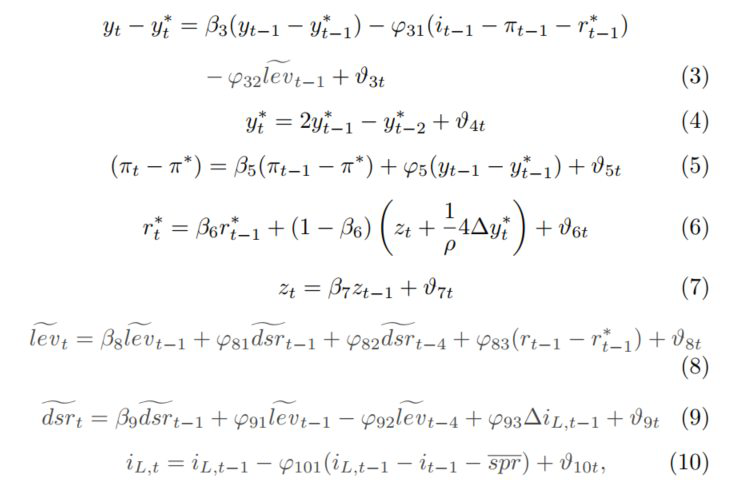
\includegraphics[scale=0.60]{LW_financial_cycles.png}
%\caption {\tiny Taxa Natural de Juros}
\end{figure}
%
%
\section{\citet{Kiley:2015}: What Can the Data Tell Us About the Equilibrium Real Interest Rate?}
LW bayesiano
Chegamos a duas conclusões principais. Primeiro, os dados fornecem relativamente pouca informação sobre o processo de geração de dados $r^{*}$; na verdade, a distribuição posterior desse processo está muito próxima da distribuição anterior. Estes resultados contrastam fortemente com os dos processos de tendência de crescimento ou taxa natural de desemprego, para os quais os dados são muito informativos. Em segundo lugar, os deslocadores de demanda adicionais - em particular, um spread de crédito - são muito importantes para as ligações estimadas entre o produto e as taxas de juros e, portanto, para as estimativas de $r^{*}$ - implicando que pesquisas anteriores que ignoram tais fatores fornecem inferência pobre. As estimativas de r ∗ que levam em conta essa gama de considerações são mais estáveis do que outras estimativas, com $r^{*}$ no final de 2014 igual a aproximadamente 1-1 / 4 por cento.
%
%
\section{\citet{Fries:2018}: National natural rates of interest and the single monetary policy in the euro area}

Neste artigo, estimamos as taxas de juros naturais nacionais variáveis no tempo para cada uma das quatro maiores economias da área do euro - França, Alemanha, Itália e Espanha - desde o início do euro em 1999. Filtramos essas variáveis não observadas condicionalmente em um modelo estilizado conjunto dessas quatro economias e suas interações. Encontramos primeiro evidências de uma tendência comum de declínio dos quatro r ∗ nacionais nos últimos 15 anos. Com exceção de alguns episódios de curta duração, sendo o último durante a recessão pós-Lehman, as diferenças no r national nacional entre os países permaneceram relativamente contidas e geralmente abaixo de 1 ponto percentual. No entanto, as taxas de juro reais de curto prazo (1 ano) divergiram acentuadamente durante a crise soberana da área do euro, reflectindo o aumento dos spreads de crédito soberano dos países do sul. Em seguida, calculamos as medidas específicas de cada país da diferença da taxa de juros real, a diferença entre a taxa real ex ante local e a taxa natural nacional estimada. De acordo com esta métrica, a política monetária única não foi comum entre os países membros ao longo de vários episódios, principalmente no clímax da crise na área do euro. Ao mesmo tempo em que garantiu uma postura neutra em relação às economias centrais, revelou-se fortemente desinflacionário na Espanha e na Itália de meados de 2011 ao final de 2012. Eventualmente, todos os quatro desvios das taxas de juros reais nacionais convergiram para cerca de -1\% ao longo dos anos de 2014 –2016, testemunhando uma orientação de política única mais consistente e expansionista em toda a área, à medida que o Eurosistema embarcou de forma mais decisiva em programas não convencionais.

Nossa estimativa produz valores plausíveis e significativos para todos os parâmetros-chave, especialmente as inclinações das curvas de Phillips e IS. Obtemos medidas variáveis no tempo das variáveis latentes não observadas no modelo: as taxas de juros naturais nacionais e os desvios das taxas de juros derivadas, os desvios do produto nacional e as taxas associadas de crescimento do produto potencial. Em primeiro lugar, descobrimos que as quatro taxas naturais nacionais flutuaram amplamente em torno de uma tendência global de declínio nos últimos 15 anos, um resultado consistente com as descobertas de Holston et al. (2016). As médias transversais de fato oscilavam entre 3,5\% em 2000 e -1,5\% em 2012, finalmente para atingir um nível próximo (mas abaixo) de zero em 2016. Antes da crise de 2008, r ∗ nacional também tendia a se mover cada vez mais, conforme a dispersão transversal diminuiu de -1,3\% em 2000 para -0,4\% em 2007. A crise financeira mundial desencadeada pelo colapso do Lehman Brothers e a recessão que se seguiu derrubou as taxas naturais em todos os quatro países, para cerca de -1\% . Embora tenham recuperado rapidamente depois disso, as suas trajetórias divergiram de novo em certa medida em 2010 e 2011. As taxas naturais nacionais permaneceram principalmente em território negativo durante a crise da dívida soberana da área do euro, atingindo um mínimo no segundo semestre de 2012, em quase -2\% em França e cerca de -1,5\% nos outros três países. Os r ∗ nacionais acabaram por se estabilizar em níveis ligeiramente negativos em todas as economias desde meados de 2015. Assim, uma vez que as taxas de juro reais reais de 1 ano divergiram acentuadamente durante a crise da área do euro, os desvios das taxas de juro nacionais estimados apontam para posturas de política monetária eficazes bastante diferenciadas nos quatro países ao longo dos anos 2011-2013. No geral, nossas estimativas sugerem que a política monetária única foi quase neutra na França no período pós-2009, enquanto
efeitos significativamente restritivos na Itália e Espanha em 2011-2012 e tem sido bastante expansionista na Alemanha desde 2013.

Contribuímos para três vertentes da literatura e debates políticos atuais. Primeiro, nosso estudo fornece uma ilustração de como usar o conceito de taxas de juros naturais para informar os formuladores de políticas. Em comparação com estudos anteriores, o nosso é o primeiro a estimar as taxas naturais para cada país membro da área do euro num enquadramento consistente. As nossas conclusões, portanto, lançam uma nova luz sobre o debate sobre a fragmentação financeira da área durante a década de 2010 e a relevância de uma política monetária "tamanho único" neste ambiente estressado caracterizado pelos choques amplamente assimétricos do pânico da dívida soberana.

Em segundo lugar, nossas estimativas de taxas de juros naturais para quatro grandes economias europeias também fornecem evidências úteis para o debate em curso sobre taxas reais baixas após a crise e a hipótese de estagnação secular.

\chapter{Modelos com Time Series}
%
%
\section{\citet{DelNegro:2019}: Global trends in interest rates}

Para responder a essas questões, estudamos a dinâmica conjunta das taxas de juros de curto e longo prazo, inflação e consumo para sete economias agora avançadas desde 1870. Fazemos isso por meio de um modelo de série temporal flexível - um vetor de autorregressão (VAR) com tendências. Essa ferramenta econométrica nos permite usar a teoria econômica para modelar e interpretar as relações de longo prazo entre as variáveis, enquanto permanecemos agnósticos sobre se essas restrições se mantêm em outras frequências. Por exemplo, a ausência de oportunidades de arbitragem no longo prazo implica que podemos interpretar a tendência comum estimada das taxas de juros reais entre os países como a tendência da taxa de juros real mundial. O mesmo referencial teórico também sugere uma decomposição dessa tendência em alguns de seus fatores potenciais, como o crescimento do consumo global.

As taxas de juros em nosso conjunto de dados referem-se a títulos do governo ou substitutos próximos, que são relativamente seguros e líquidos em comparação com outros ativos de emissão privada. Portanto, permitimos que o rendimento de conveniência para a segurança e a liquidez oferecidas por esses ativos “seguros” desempenhem um papel na condução da seção internacional de retornos. Para medir esse rendimento de conveniência, a análise empírica também inclui o rendimento de títulos corporativos Baa da Moody's para os Estados Unidos.

Quatro resultados principais emergem de nossa análise empírica. Em primeiro lugar, a tendência estimada da taxa de juros real mundial manteve-se estável em torno de valores um pouco abaixo de $2\%$ ao longo da década de 1940. Aumentou gradualmente após a Segunda Guerra Mundial para um pico de cerca de $3\%$ no final dos anos setenta, mas tem diminuído desde então, caindo para quase zero em 2016, o último ano de dados disponível. O nível exato dessa tendência é cercado por uma incerteza substancial, mas a queda nas últimas décadas é estimada com precisão. Um declínio dessa magnitude não tem precedentes em nossa amostra. Nem mesmo ocorreu durante a Grande Depressão na década de 1930.

Em segundo lugar, a tendência da taxa de juros mundial desde o final da década de 1970 coincide essencialmente com a dos EUA. Em outras palavras, a tendência dos EUA é a tendência global nas últimas quatro décadas. Na verdade, esse tem sido cada vez mais o caso para quase todos os outros países em nossa amostra: as tendências idiossincráticas estão desaparecendo desde o final dos anos 1970. Essa convergência nas taxas de juros entre os países é indiscutivelmente o resultado da crescente integração nos mercados internacionais de ativos.

Terceiro, a tendência de declínio da taxa de juros real mundial nas últimas décadas é impulsionada em extensão significativa por um aumento nos convenience yield, que aponta para um desequilíbrio crescente entre a demanda global por segurança e liquidez e sua oferta. Essa contribuição está especialmente concentrada no período desde meados da década de 1990, apoiando a visão de que a crise financeira asiática de 1997 e a inadimplência da Rússia em 1998, com o subsequente colapso do LTCM, foram pontos de inflexão importantes no surgimento de desequilíbrios globais.

Quarto, um declínio global na taxa de crescimento do consumo per capita, possivelmente vinculado a mudanças demográficas, é outro fator notável que está empurrando as taxas reais globais para baixo. Sua contribuição é comparável em magnitude à do convenience yield desde 1980, mas apenas cerca de metade da importância nos últimos vinte anos (e estimada com menos precisão).

Uma implicação importante dessas descobertas é que o persistente
os ventos contrários macroeconômicos decorrentes da crise financeira, incluindo os efeitos das políticas extraordinárias que foram postas em prática para combatê-la, estão longe de ser a única causa do ambiente de juros baixos. Forças seculares de longa data conectadas com um declínio no crescimento econômico desde o início dos anos 1980 e o aumento dos convenience yield desde o final dos anos 1990 também parecem ser os culpados cruciais, embora essas tendências possam ter sido exacerbadas pela crise.

Nossos resultados estão intimamente alinhados com esta literatura ao enfatizar o importante papel dos convenience yield na geração de retornos internacionais. Eles são complementares porque nos concentramos na contribuição desses fatores para impulsionar o comovimento internacional das taxas de juros em baixas frequências e por um período de tempo muito mais longo. Portanto, podemos abordar explicitamente a questão de como a dimensão global da demanda por segurança e liquidez moldou o declínio secular das taxas reais em todo o mundo nas últimas décadas, o que também nos permite fazer contato com a vasta literatura sobre r * discutido acima.

Dez anos após a fase mais aguda da crise financeira global, as taxas de juros permanecem em níveis historicamente baixos ou próximos a muitos para muitos países. Estudamos os fatores seculares desse ambiente de taxas de juros baixas através das lentes de uma autorregressão vetorial com tendências comuns, usando dados históricos de sete países a partir de 1870. Descobrimos que a tendência da taxa de juros real mundial segura, que era praticamente estável em um pouco abaixo de $2\%$ por mais de cem anos, caiu significativamente nas últimas três décadas. Esta tendência global, que identificamos como o componente comum nos movimentos de baixa frequência dos rendimentos reais sobre ativos seguros e líquidos (títulos do governo ou substitutos próximos) nas sete economias em nossa amostra, se assemelha muito às tendências para todas as economias avançadas, incluindo os Estados Unidos, no período recente. Descobrimos que as tendências específicas de cada país praticamente desapareceram desde os anos 1970.

Esse declínio secular nas taxas reais globais é impulsionado principalmente por um aumento no prêmio que os investidores internacionais estão dispostos a pagar para manter ativos seguros e líquidos, bem como pelo menor crescimento econômico em todo o mundo. A última tendência tem exercido pressão descendente sobre as taxas reais desde cerca de 1980, possivelmente ligada a mudanças demográficas, enquanto a primeira surgiu no final da década de 1990. Este momento aponta para a escassez de ativos seguros no contexto de um excesso de poupança global como uma força secular fundamental por trás do ambiente de taxas de juros baixas.
%
%
\section{\citet{Johannsen:2018}: A time series model of interest rates with the effective lower bound}
Este artigo modela as taxas de juros nominais, juntamente com outros dados macroeconômicos, usando um modelo de série temporal flexível que incorpora explicitamente o limite inferior efetivo (ELB) nas taxas de juros nominais. Empregamos um dispositivo de modelagem a que nos referimos como “shadow rate” - a taxa de juros nominal que prevaleceria na ausência do ELB.

Usamos nossa abordagem para estimar um modelo de ciclo de tendência de dados dos EUA sobre taxas de juros, atividade econômica e inflação em uma amostra que inclui o período recente no ELB. Desde a crise financeira global de 2008, as taxas de juros reais têm estado historicamente baixas, o que levou alguns a argumentar que o nível de longo prazo da taxa de juros real caiu. Incorporamos a estimativa das taxas reais de tendência em um modelo de volatilidade estocástica cujas estimativas veem quedas recentes nas taxas reais como amplamente cíclicas
na natureza.

Como resultado, nossas estimativas da tendência da taxa real são menos variáveis do que as relatadas. Encontramos uma incerteza considerável em torno das estimativas da taxa real no longo prazo. À luz das amplas faixas de incerteza em torno das estimativas de tendência, a modesta tendência de queda em nossas estimativas de tendência da taxa real não é significativa.Como resultado, nossas estimativas da tendência da taxa real são menos variáveis do que as relatadas. Encontramos uma incerteza considerável em torno das estimativas da taxa real no longo prazo. À luz das amplas faixas de incerteza em torno das estimativas de tendência, a modesta tendência de queda em nossas estimativas de tendência da taxa real não é significativa.

Modelar explicitamente o ELB tem grandes efeitos na inferência sobre taxas de juros esperadas fora da amostra nos últimos anos. Nossas shadow rate estimadas são menores do que o ELB por definição, e nosso modelo oferece caminhos previstos para as taxas de juros de curto prazo futuras que incluem períodos prolongados no ELB. Comparamos as previsões de taxas de juros de nosso modelo com as previsões da Survey of Professional Forecasters (SPF) e descobrimos que nosso modelo tem um desempenho melhor do que o SPF em horizontes mais longos.

No ELB, a shadow rate é uma variável de estado não observada que importa para a previsão de resultados futuros na taxa de juros e outras variáveis. Quando a taxa de referência está acima do ELB, a shadow rate é igual à taxa de referência e, portanto, também observada. Em ambos os casos, as inovações na shadow rate podem ser interpretadas como refletindo mudanças na política monetária - sejam elas implementadas na forma de variações convencionais na taxa de juros quando o ELB não é vinculativo, ou por meio de ferramentas não convencionais (como compras de ativos ou a termo orientação) caso contrário. Nesse espírito, estimamos as respostas de impulso a choques de política monetária, que são identificados pela imposição de restrições de curto prazo às surpresas da shadow rate.

Além disso, nosso modelo de volatilidade estocástica gera respostas de impulso que variam no tempo: Nossos choques de política são identificados a partir de restrições convencionais de curto prazo impostas à estrutura de covariância dos erros de previsão de forma reduzida do modelo. À medida que a importância relativa dos choques nas tendências e nos ciclos muda, também muda a estrutura de covariância dos erros de previsão de forma reduzida do modelo, bem como a persistência de seus efeitos.

Descobrimos que os choques de política monetária identificados a partir de inovações na taxa de sombra afetam os spreads de rendimento de forma mais marcante quando o ELB é vinculativo, consistente com a noção de que as taxas de sombra capturam os efeitos de políticas não convencionais. É importante ressaltar que nossos resultados sugerem que uma acomodação monetária adicional durante o período mais profundo da recessão mais recente teria fornecido mais estímulo do que a acomodação monetária fornecida em outros momentos.

Neste artigo, desenvolvemos uma metodologia para contabilizar o ELB em modelos de séries temporais de taxas de juros nominais. Nosso método torna os modelos lineares gaussianos acessíveis ao ELB, mas também pode ser aplicado a modelos de parâmetros variáveis no tempo que são apenas condicionalmente lineares. Por exemplo, nossa aplicação empírica é baseada em um modelo de componentes não observados com volatilidade estocástica. Demonstramos como estimar os parâmetros e estados latentes de tal modelo com um amostrador MCMC Bayesiano padrão.

A consideração adequada do ELB tem, evidentemente, efeitos drásticos nas previsões das taxas de juros. Mesmo entre os preditores que aderem ao ELB, nossa abordagem de shadow rate se sai bem em comparação com vários concorrentes. Também estimamos uma tendência comum das taxas reais, definida como uma previsão de longo prazo da taxa de juros real, e não encontramos nenhum declínio significativo na tendência da taxa real desde os anos 1990.

Finalmente, nosso modelo gera respostas de impulso que variam no tempo a choques de política monetária. Descobrimos que os choques de política monetária identificados a partir de inovações na taxa de sombra afetam os spreads de rendimento de forma mais marcante quando o ELB é vinculativo, consistente com a noção de que as taxas de sombra capturam os efeitos de políticas não convencionais. É importante ressaltar que nossos resultados sugerem que a acomodação monetária durante as profundezas da recessão mais recente teria fornecido mais estímulo do que em outros momentos.
%
%
\section{\citet{Hamilton:2016}: The Equilibrium Real Funds Rate: Past, Present, and Future}

Examinamos o comportamento, os determinantes e as implicações do nível de equilíbrio da taxa real de fundos federais, definida como a taxa consistente com o pleno emprego e inflação estável no médio
prazo. Tiramos três conclusões principais. Em primeiro lugar, a incerteza em torno da taxa de equilíbrio é grande e sua relação com a tendência de crescimento do PIB muito mais tênue do que se acredita. Nossa análise narrativa e econométrica usando dados de vários países e remontando ao século 19 suporta uma ampla gama de estimativas centrais plausíveis para o nível atual da taxa de equilíbrio, de um pouco mais de $0\%$ ao consenso pré-crise de $2\%$. Em segundo lugar, apesar dessa incerteza, somos céticos em relação à visão da “estagnação secular” de que a taxa de equilíbrio permanecerá próxima de zero por muitos anos. As evidências de estagnação secular antes da crise de 2008 são fracas, e a decepcionante recuperação pós-2008 é melhor explicada por ventos contrários prolongados, mas em última análise temporários, causados pelo excesso de oferta de moradias, desalavancagem das famílias e dos bancos e contenção fiscal. Uma vez que esses ventos contrários diminuíram no início de 2014, o crescimento dos EUA de fato acelerou a um ritmo bem acima do potencial. Em terceiro lugar, a incerteza em torno da taxa de equilíbrio implica que uma regra de política monetária com mais inércia do que implícita nas versões padrão da regra de Taylor poderia estar associada a menores desvios do produto e da inflação dos objetivos do Fed. Nossas simulações usando o modelo FRB / US da equipe do Fed mostram que o reconhecimento explícito dessa incerteza resulta em um caminho de normalização posterior, mas mais íngreme para a taxa de fundos em comparação com o "ponto" mediano no Resumo de Projeções Econômicas do FOMC.

Neste artigo, abordamos a questão de um “novo neutro” examinando a experiência de um grande número de países, embora com foco nos EUA. descrevemos os dados e procedimentos que usaremos para construir as taxas reais ex-ante usadas em nossa análise. Esses dados remontam a dois séculos para alguns países e também incluem dados mais detalhados sobre a experiência mais recente das economias da OCDE. Também observamos a estratégia que freqüentemente usamos para fazer afirmações empíricas sobre a taxa de equilíbrio: na maior parte, olharemos para as médias ou médias móveis de nossas medidas de taxas reais; em nenhum momento iremos estimar um modelo estrutural.

Consideramos as médias móveis como medidas (ruidosas) da taxa de equilíbrio e da taxa de crescimento da tendência. Usando observações de longas séries de tempo para os Estados Unidos e também a experiência dos países da OCDE desde 1970, investigamos a relação entre taxas reais seguras e tendência de crescimento do produto. Descobrimos algumas evidências de que taxas de crescimento de tendência mais altas estão associadas a taxas reais médias mais altas. No entanto, essa descoberta é sensível à amostra particular de dados que é usada. E mesmo para as amostras com relação positiva, a correlação entre o crescimento e as taxas médias é modesta. Concluímos que fatores além das mudanças na tendência da taxa de crescimento são centrais para explicar por que a taxa real de equilíbrio muda ao longo do tempo.

Fornecemos uma história narrativa dos determinantes da taxa real nos EUA tentando identificar os principais fatores que podem ter movido a taxa de equilíbrio ao longo do tempo. Concluímos que as mudanças ao longo do tempo nas taxas de desconto pessoal, regulamentação financeira, tendências na inflação, bolhas e ventos contrários cíclicos tiveram efeitos importantes sobre a taxa real observada em média ao longo de qualquer década. Discutimos a hipótese da estagnação secular em detalhes. No geral, consideramos isso pouco convincente, argumentando que provavelmente confunde uma recuperação atrasada com uma demanda agregada cronicamente fraca. Nossa análise sugere que o ciclo atual pode ser semelhante aos dois últimos, com uma “normalização” tardia tanto da economia quanto da taxa de fundos. Nossa abordagem narrativa sugere que a taxa de equilíbrio pode ter caído, mas provavelmente apenas ligeiramente. O crescimento da tendência presumivelmente menor implica uma taxa de equilíbrio abaixo da média de $2\%$ que prevaleceu recentemente, talvez em algum lugar na faixa de $1\%$ a $2\%$.

Realizamos algumas análises estatísticas dos dados de longo prazo dos EUA e descobrimos, de acordo com nossa história narrativa, bem como com resultados empíricos encontrados por outros pesquisadores em conjuntos de dados do pós-guerra, que nós pode rejeitar a hipótese de que a taxa de juros real converge ao longo do tempo para alguma constante fixa. Encontramos uma relação que parece estável. A taxa real dos EUA é cointegrada com uma medida que é semelhante à mediana de uma média de 30 anos das taxas reais em todo o mundo. Quando a taxa dos EUA está abaixo da taxa mundial de longo prazo (como no início de 2015), podemos ter alguma confiança de que a taxa dos EUA vai subir, consistente com a conclusão de nossa análise narrativa. O modelo prevê que a taxa real de longo prazo dos EUA e do mundo se estabilize em um valor em torno de meio por cento em cerca de três anos. No entanto, como a própria taxa mundial também é não estacionária, sem tendência clara de reverter para uma média fixa, a incerteza associada a essa previsão torna-se maior à medida que tentamos olhar para o futuro.
%
%
\section{\citet{Rudebusch:2019}: A New Normal for Interest Rates? Evidence from Inflation-Indexed Debt}

Dadas essas armadilhas potenciais de uma estimativa baseada em macro, nos voltamos para modelos financeiros e dados para fornecer uma abordagem alternativa para estimar a taxa de juros real de equilíbrio. Usamos os preços da dívida indexada à inflação, a saber, U.S. Treasury Inflation-Protected Securities (TIPS). Esses títulos têm pagamentos de cupom e principal que se ajustam às variações do Índice de Preços ao Consumidor (IPC) e, assim, compensam os investidores pela erosão de poder compra devido à inflação. Os preços desses títulos podem fornecer uma leitura bastante direta dos rendimentos reais desde 1997, quando o programa TIPS foi lançado. Assumimos que as expectativas de longo prazo embutidas nos preços de TIPS refletem as visões dos participantes do mercado financeiro sobre o estado estacionário da economia, incluindo a taxa de juros de equilíbrio. Nossa medida da taxa natural baseada em finanças tem várias vantagens potenciais em relação às estimativas baseadas em macro. Mais notavelmente, nossa medida da taxa de equilíbrio não depende da obtenção de uma especificação correta da dinâmica do produto e da inflação - ao contrário de estimativas anteriores que dependem de uma representação macroeconômica específica. Além disso, nossa medida pode ser obtida em tempo real na mesma alta frequência que os dados do preço do título subjacente e é baseada em dados do mercado financeiro e, portanto, é naturalmente foward-looking.

Ainda assim, o uso de TIPS para medir a taxa de juros real de curto prazo em estado estacionário apresenta seus próprios desafios empíricos. Uma dificuldade é que os preços dos títulos indexados à inflação incluem um prêmio de prazo real. Dada a inclinação geralmente ascendente da curva de rendimento TIPS, o prêmio de prazo real parece positivo em média, mas sua variabilidade é desconhecida. Além disso, apesar do valor nocional bastante elevado de TIPS em circulação, esses títulos provavelmente enfrentam um risco de liquidez considerável.

Para estimar a taxa de juros de equilíbrio na presença de liquidez e prêmios de prazo real, usamos modelos de estrutura a termo dinâmica livre de arbitragem de rendimentos reais. A formulação teórica livre de arbitragem do modelo fornece a identificação de um prêmio de prazo real variável no preço de TIPS. Além disso, nosso modelo é estimado usando os preços de títulos individuais, em vez da entrada mais comum de rendimentos de curvas sintéticas ajustadas

Para robustez, consideramos dois modelos dinâmicos de estrutura a termo diferentes. Um é mais padrão, sem tratamento explícito separado do prêmio de liquidez - riscos de prazo e de liquidez são modelados implicitamente juntos. O segundo modelo é ampliado com um fator de risco de liquidez explícito. Este modelo identifica um fator de liquidez geral de TIPS e a carga de cada título individual nesse fator a partir da seção transversal dos preços de TIPS ao longo do tempo - com cada título possuindo um tempo diferente desde a emissão e até o vencimento.

Usando modelos e dados macroeconômicos, muitos pesquisadores investigaram a contribuição para a tendência de baixa dos rendimentos nas últimas décadas a partir de uma taxa de juros real de equilíbrio em queda. No entanto, a incerteza sobre a especificação macroeconômica correta levou alguns a questionar a validade das estimativas macroeconômicas resultantes da taxa natural. Evitamos esse debate introduzindo uma medida da taxa real de equilíbrio baseada em finanças, obtida exclusivamente de modelos dinâmicos de estrutura a termo estimados com base nos preços de títulos indexados à inflação. Ajustando os prêmios de liquidez do TIPS e os prêmios de prazo real, descobrimos as expectativas dos investidores quanto à taxa de juros curta real sem atrito subjacente para o período de cinco anos, começando cinco anos à frente. Nossa medida resultante da taxa natural de juros exibe um declínio gradual nas últimas duas décadas para um nível essencialmente zero. Além disso, as projeções do modelo sugerem que a taxa natural provavelmente permanecerá bastante baixa por algum tempo.

Vemos nossa análise de taxa de equilíbrio baseada em finanças como um complemento às anteriores macrobaseadas. Como as estimativas baseadas em macro, uma estimativa baseada em finanças também está sujeita a críticas sobre a especificação do modelo e o conteúdo de informação dos dados disponíveis. À luz de tais críticas, a faixa de incerteza associada a uma estimativa baseada em finanças não parece ser necessariamente menor do que aquela em torno das estimativas baseadas em macro. No entanto, os modelos e dados subjacentes nas duas abordagens são tão diferentes que os intervalos de confiança provavelmente também não estão correlacionados, o que sugere um valor substancial da construção e comparação de estimativas baseadas em finanças e macro. É claro que uma abordagem conjunta que combine dados macroeconômicos e do mercado financeiro parece ser particularmente promissora para pesquisas futuras. Na verdade, nossa medida poderia ser incorporada a uma análise macroeconômica e financeira conjunta expandida - particularmente com o objetivo de compreender melhor os determinantes da nova normalidade mais baixa para as taxas de juros.
%
%
\section{\citet{Lubik:2015}: Calculating the Natural Rate of Interest: A Comparison of Two Alternative Approaches}

Um modelo autoregressivo de vetor de parâmetro variável no tempo (TVPVAR) é uma estrutura flexível para estudar as relações complexas entre os dados macroeconômicos. É um modelo de série temporal que explica a evolução das variáveis econômicas em função de seus próprios valores defasados e choques aleatórios. O que distingue um TVPVAR da abordagem VAR mais padrão é que os parâmetros do modelo, nomeadamente os coeficientes de defasagem e as variâncias dos choques económicos, podem variar ao longo do tempo. Esta estrutura é, portanto, capaz de capturar uma variedade de comportamentos não lineares que são aparentes em séries temporais macroeconômicas, como movimentos assimétricos de variáveis ao longo do ciclo de negócios ou o declínio geral da volatilidade macroeconômica desde meados da década de 1980.

Esta última questão é especialmente pertinente à questão do comportamento da taxa natural de juros. Como mostram os números acima, parece haver um declínio secular na taxa real e sua contraparte natural, conforme estimado por Laubach e Williams, bem como mudanças na volatilidade do primeiro durante o período da amostra. Além disso, a existência do limite inferior zero na taxa de juros nominal introduz, por si só, não linearidade nas relações macroeconômicas. Essas considerações, portanto, tornam um TVP-VAR uma estrutura atraente para capturar a taxa natural.

O que distingue esta abordagem do método de Laubach e Williams é que o TVP-VAR impõe muito menos de uma estrutura econômica. Enquanto Laubach e Williams postularam relações econômicas entre as principais variáveis macroeconômicas que podem ou não ser suportadas, um TVP-VAR é amplamente agnóstico nessa dimensão. Ele simplesmente captura o co-movimento entre essas variáveis de uma maneira flexível. A identificação da taxa natural em Laubach e Williams repousa criticamente nas suposições que regem
modelo econômico subjacente.

Estimamos um simples TVP-VAR para três variáveis— a taxa de crescimento do produto interno bruto real, a taxa de inflação PCE e a medida da taxa de juros real usada por Laubach e Williams - durante o período de amostra de 1961 até o segundo trimestre de 2015. Conforme discutido acima, a abordagem TVP-VAR é bem adequado para capturar as características seculares e de ciclo de negócios desse intervalo de dados. Propomos como medida da taxa natural de juros a previsão condicional de longo prazo da taxa real observada. Nosso horizonte de tempo escolhido é de cinco anos, e a previsão é calculada para cada ponto de dados desde 1967. Em contraste com os VARs de coeficiente fixo estacionário, as previsões não revertem para a média da amostra porque os coeficientes do TVP-VAR seguem caminhos aleatórios.

\chapter{Modelos DSGE}
%
%
\section{\citet{Neiss:2003}: The Real-Interest Rate gap as Inflation Indicator}
Este artigo examinou o que um modelo DSGE tem a dizer sobre o hiato da taxa de juros real como um indicador de inflação. Uma lacuna do conceito é que ele requer a construção de uma série de taxas reais naturais “não observáveis”. No entanto, o mesmo é verdade para o conceito de hiato do produto, e nossos resultados sugerem que a série do hiato do produto com frequência construída pode ser enganosa. Nessas circunstâncias, uma série de desvios da taxa de juros real é útil para avaliar a orientação da política monetária e a pressão inflacionária. Seus resultados sugerem que há benefícios em permitir movimentos da taxa natural ao modelar a inflação e basear a construção de séries de taxas naturais na teoria econômica. Os benefícios quantitativos podem ser modestos, entretanto, por causa do baixo grau de variação cíclica na taxa natural.

Este artigo desenvolve um modelo DSGE de preço fixo para examinar o comportamento da taxa de juros real natural e do gap da taxa de juros real. Todos os modelos DSGE fornecem implicitamente modelos do gap da taxa de juros real. Em modelos de preços flexíveis, o comportamento da diferença da taxa real é trivial - é zero a cada período porque a taxa de juros real é a taxa natural.

Incluímos a formação de capital e os choques de preferência, bem como outros elementos ausentes dos artigos acima, como a utilidade não separável no tempo. Também consideramos mais de uma especificação de definição de preço.

Os dois principais resultados deste artigo são que a taxa real natural não flutua muito ao longo do ciclo de negócios e, portanto, a taxa real é uma proxy razoável para a diferença da taxa de juros real; e que, em contraste, a variação do produto potencial é importante na frequência do ciclo de negócios. Esses resultados são consistentes com os pontos (i) e (ii) acima e têm implicações importantes para a modelagem da inflação e para as regras de política.

Sob preços flexíveis, as taxas de juros reais e naturais coincidem independentemente da regra de política monetária. Mas a política monetária tem efeitos reais quando os preços são rígidos, de modo que a especificação da regra de política terá implicações para a diferença da taxa de juros real. Examinamos as propriedades da diferença da taxa de juros real sob uma variedade de regras diferentes

Resposta da taxa natural de juros a choques de tecnologia e de preferência.
\begin{figure}[H]
\centering
%\includegraphics[scale=0.60]{Figura Neiss.jpg}
\includegraphics[scale=0.60]{Figuras/Figura Neiss.jpg}
%\caption {\tiny Taxa Natural de Juros}
\end{figure}

Tech shoch: No caso sem capital, um choque tecnológico aumenta a produção e o consumo hoje em mais do que em períodos futuros. A restrição de oferta agregada do período atual sobre a capacidade de consumo da família foi relaxada, e a restrição em períodos futuros foi relaxada por uma quantidade menor e decrescente. As famílias iriam gostar de suavizar seu consumo do produto mais alto (especialmente dada a formação de hábito em suas preferências) e tentam adiar muito de seu consumo mais alto. Mas, em equilíbrio, toda a produção deve ser consumida hoje. A taxa de juros real natural diminui para garantir que isso ocorra

Quando o capital pode variar, o investimento aumenta porque o choque tecnológico aumenta a lucratividade da produção. Isso tende a aumentar $r_t^{*}$. A pressão compensatória vem do desejo das famílias de economizar parte da renda extra e do desincentivo ao investimento rápido dos custos de ajuste. O efeito líquido é uma queda em $r_t^{*}$, embora menor do que no caso sem capital.

Preference shock: Ao contrário de um choque de política monetária, isso afeta os valores das variáveis reais sob a flexibilidade de preços. O choque aumenta a demanda de consumo. Com o capital totalmente flexível, apenas uma pequena mudança na taxa real é necessária para facilitar um declínio no investimento e abrir espaço para um consumo maior; portanto, a resposta limitada de $r_t^{*}$. Se não houver capital ou se as empresas enfrentarem grandes custos de ajuste, a taxa real deve aumentar mais para amortecer o aumento do consumo.

Agora nos voltamos para o caso do rigidez de preço e examinamos a resposta do gap da taxa de juros real. Resposta da taxa natural de juros a choques de tecnologia e de preferência.

\begin{figure}[H]
\centering
%\includegraphics[scale=0.60]{Figura Neiss2.jpg}
\includegraphics[scale=0.60]{Figuras/Figura Neiss2.jpg}
%\caption {\tiny Taxa Natural de Juros}
\end{figure}

O efeito de um choque tecnológico. O choque gera um aumento na diferença da taxa de juros real - um aperto de política eficaz - por dois motivos. Primeiro, a taxa natural cai e, portanto, para uma dada taxa de juros real, a política monetária é mais rígida. Em segundo lugar, a regra de política responde ao nível de produto e, portanto, um choque de produtividade induz um aumento na taxa de juros nominal e, portanto, real.

Um choque IS, entretanto, aumenta a taxa real e natural. Assim, em contraste com o caso do choque tecnológico, a resposta política - um aperto em resposta a um produto mais alto - tende a conter a abertura de um hiato da taxa real. No entanto, o aumento da taxa real é menor do que o aumento da taxa natural e, portanto, a orientação geral da política é mais frouxa.

Um aperto monetário afeta apenas a taxa de juros real. A diferença da taxa real, portanto, aumenta um por um com a taxa real. As respostas do produto e do hiato do produto são idênticas porque a política monetária não pode afetar o PIB potencial.

%
%
\section{\citet{Orphanides:2002}: Robust Monetary Policy Rules with Unknown Natural Rates }
Policymakers não conhecem os valores dessas taxas naturais em tempo real, isto é, quando tomam decisões políticas. De fato, mesmo em retrospectiva, há uma incerteza considerável em relação às taxas naturais de desemprego e juros, e ambiguidade sobre como melhor modelar e estimar as taxas naturais.

Esses problemas de mensuração parecem ser particularmente agudos na presença de mudanças estruturais quando as taxas naturais podem variar de maneira imprevisível, fazendo com que as estimativas das taxas naturais estejam sujeitas a um aumento da incerteza.

Empregamos um modelo trimestral foward-looking da economia norte-americana para examinar as propriedades de desempenho e robustez de regras de política de taxa de juros simples na presença de medidas precárias em tempo real das taxas naturais de juros e desemprego. Um aspecto fundamental de nossa investigação é o reconhecimento de que os formuladores de políticas podem estar incertos quanto aos verdadeiros processos geradores de dados que descrevem as taxas naturais de desemprego e juros e a extensão do problema de inconsistência que eles enfrentam. Como resultado, aplicações padrão de equivalência certeza baseadas no problema clássico de controle linear-quadrático-Gaussiano não se aplicam.

Nós achamos que os custos de subestimar a extensão da mensuração da taxa natural excedem significativamente os custos de superestimação. Adoção de regras de política otimizadas sob a falsa suposição de que as percepções errôneas em relação às taxas naturais provavelmente serão pequenas, o que é particularmente custoso em termos de estabilização da inflação e do desemprego.

Quando os formuladores de políticas não possuem uma estimativa precisa da magnitude das percepções errôneas em relação às taxas naturais, uma estratégia robusta é agir como se a incerteza que enfrentassem fosse maior do que suas estimativas básicas sugerem que pode ser. Mostramos que negligenciar essas considerações pode facilmente resultar em políticas com desempenhos de estabilização consideravelmente piores do que o previsto.

Nossos resultados apontam para uma estratégia simples e eficaz que é uma solução robusta para as dificuldades associadas às percepções errôneas da taxa natural. Isso é para adotar, como diretrizes para política monetária, regras de diferenças nas quais a taxa de juros nominal de curto prazo é aumentada ou diminuída de seu nível existente em resposta à inflação e mudanças na atividade econômica. Essas regras, que não requerem conhecimento das taxas naturais de juros e desemprego e, consequentemente, são imunes a percepções errôneas nesses conceitos, emergem como a solução para um exercício de controle robusto a partir de uma família mais ampla de especificações de regras de política.

Este artigo reexaminou criticamente a utilidade das taxas naturais de juros e desemprego no cenário da política monetária. Nossos resultados sugerem que subestimar a falta de confiabilidade das estimativas em tempo real das taxas naturais pode levar a políticas que são muito muito caras em termos do desempenho de estabilização da economia. De fato, nossas análises e conclusões são baseadas inteiramente em modelos em que os desvios das taxas naturais são os principais propulsores da inflação e do desemprego. Em vez disso, argumentamos que a incerteza sobre as taxas naturais em tempo real recomenda não depender excessivamente desses indicadores intrinsecamente ruidosos para decisões de política monetária.
%
%
\section{\citet{Edge:2008}: Natural rate measures in an estimated DSGE model of the U.S. economy  }
Estima um DSGE para economia dos EUA, utilizando de técnicas de econometria bayesiana. Eles usam seu modelo estimado para gerar e interpretar estimativas baseadas em modelo do produto potencial e a taxa natural de juros. Em modelos DSGE estimados como o nosso, os caminhos históricos para choques estruturais não observados são estimados além dos valores dos parâmetros. Consequentemente, podemos derivar estimativas históricas de variáveis de taxa natural, que, de maneira importante, têm interpretações estruturais muito claras.

Em sua discussão sobre nossas estimativas baseadas em modelo de produto potencial (e, portanto, o hiato do produto) e a taxa natural de juros, fornecemos vários exemplos de como nosso modelo pode auxiliar sua compreensão da macroeconomia dos EUA nos últimos 20 anos. Além disso, também consideramos como as estimativas do nosso modelo do hiato do produto e a taxa de juros natural diferem daquilo que consideramos como sabedoria convencional. Descobrimos que, embora a trajetória estimada do modelo da taxa natural de juros seja notavelmente mais volátil do que as estimativas derivadas (e nossa visão da sabedoria convencional), a trajetória estimada do modelo do hiato do produto compartilha algumas características importantes com outras produções mais tradicionais. estimativas baseadas em função.

A taxa natural de juros implícita em nosso modelo é muito volátil. Além de sua plausibilidade para os formuladores de políticas, pode haver mais questões relacionadas a flutuações na taxa de juros natural e seu papel no processo político em um modelo típico de DSGE como o nosso. Em particular, nosso modelo baseia-se na persistência de hábito para gerar respostas persistentes, em forma de hump-shaped, de variáveis-chave de gastos para os fundamentos. É bem sabido que essa especificação de preferências tem algumas implicações de preços de ativos intragáveis; Especificamente, esses modelos implicam substancial volatilidade na taxa de juros real livre de risco.
%
%
\section{\citet{Lopez-Salido:2009}: Money and the natural rate of interest: Structural estimates for the United States and the euro area }

Neste artigo, examinam o papel da moeda em uma estrutura geral que abrange três ambientes concorrentes: o modelo novo keynesiano  base com utilidade separável e demanda de moeda estática; utilidade inseparável entre o consumo e os saldos reais, juntamente com a formação de hábitos; e o modelo modificado para permitir custos de ajuste para manter os saldos reais. As duas últimas variantes implicam um caráter foward looking dos saldos monetários reais que transmite a moeda um papel importante como indicador de política monetária. o modelo padrão Novo Keynesian é um caso especial restritivo em que a moeda é menos informativo. Distinguimos entre esses cenários alternativos, realizando uma análise econométrica estrutural para os Estados Unidos e a área do euro. Nossas estimativas de probabilidade confirmaram o caráter foward looking da demanda por moeda. Uma das principais fontes desse comportamento voltado para o futuro é a existência de custos de ajuste de portfólio.

Ilustram como o valor da moeda aumenta em nos modelos estimados, em relação ao modelo base novo keynesiano, pela especificação da dinâmica da demanda por moeda para a qual encontramos suporte empírico. Nós nos concentramos nas ligações entre a moeda e a taxa natural e demonstramos que a moeda pode ter valor como um indicador de futuras variações na taxa natural, mesmo quando a dinâmica da inflação é vista através de uma estrutura neo-wickselliana do tipo defendido por Woodford (2003).

Neste artigo, distinguimos entre as visões alternativas do papel da moeda no mecanismo de transmissão, realizando uma análise econométrica estrutural das economias dos EUA e da área do euro. O modelo de equilíbrio geral estocástico dinâmico que estimado fornece cada variante de modelo  como um caso especial. Um resultado importante é que as estimativas de máxima verossimilhança confirmam o caráter prospectivo da demanda por moeda. Usando o modelo estimado, é capaz de demonstrar a capacidade aumentada da moeda para capturar o mecanismo de transmissão da política monetária quando a demanda por moeda tem um elemento prospectivo. Em particular, mostramos que o valor do dinheiro como proxy para as variações na taxa de juros natural e a diferença da taxa de juros real é aumentado.

A demanda por moeda é dada por:
$$\tilde{m}_t = \psi\tilde{m}_{t-1} + b_0 \tilde{y}_t + c_o \tilde{r}_t + \sum_{i=1}^{\infty} d_i E_t \tilde{rr^{*}}_t  \sum_{i=1}^{\infty} f_i E_t \{\tilde{rr}_{t+i} - \tilde{rr^{*}}_{t+i}  \} + \epsilon_t $$

Que toda a variação nos saldos reais não é decorrente de seus determinantes "convencionais" (ou seja, a renda real atual, a
taxa de juros de curto prazo atual, saldos defasados e o choque de demanda de moeda) está associado a movimentos nas defasagens de taxa de juros futura esperadas ou taxas de juros reais naturais esperadas. Notamos que a relação entre os saldos monetários reais e a taxa natural é bastante complexa, não apenas por causa da dinâmica envolvida, mas também porque a taxa natural entra com coeficientes negativos e positivos na expressão.

Essa perspectiva sobre a relação demanda por moeda destaca três vantagens da estimativa de nosso modelo estrutural por métodos de informação completa. Primeiro, as funções de demanda por moeda estimadas padrão negligenciam o comportamento prospectivo. O erro de especificação resultante ignora as informações sobre a taxa natural na demanda por moeda, em vez de atribuir a variação associada nos saldos reais a choques de demanda, ajustes defasados e respostas à renda corrente e à taxa de juros nominal. Nossa abordagem, ao contrário, isola o componente prospectivo da demanda por moeda e, portanto, oferece a perspectiva de uma estimativa consistente dos parâmetros de demanda monetária. Em segundo lugar, ao especificar explicitamente os processos de choque e o comportamento da política e, assim, o caminho implícito dos termos de expectativas que aparecem nas condições de otimalidade dos agentes, podemos extrair estimativas de taxa natural de outros determinantes inobserváveis da demanda de moeda. Terceiro, outras estimativas empíricas de séries de desvios de taxa natural e real utilizando métodos de sistemas, seja com modelos ad hoc (eg Laubach e Williams, 2003) ou modelos DSGE (eg Smets e Wouters, 2003), sacrificam informações sobre a taxa natural por não incluir saldos monetários reais no conjunto de variáveis modeladas. Nossas estimativas de sistemas, pelo contrário, incluem dinheiro na função de verossimilhança.

A taxa real de juros natural corresponde à taxa real de juros de curto prazo que prevaleceria quando a probabilidade Calvo se aproxima de 1,0, ou seja, quando todos os preços são flexíveis (e todas as empresas são foward looking). O processo de taxa natural será invariante à regra de política monetária, mas será uma função (possivelmente dinâmica) dos dois choques reais no modelo (IS (preferência) e choque tecnológico). Na aplicação aqui, a obtenção de uma série de taxa natural envolve a avaliação de nosso modelo com parâmetros que descrevem preferências e produção em seus valores estimados, resolvendo o modelo a preços flexíveis e obtendo uma representação ao estilo de Wold da taxa natural.

\section{\citet{Justiniano:2010}: Measuring the Equilibrium Real Interest Rate }

A taxa de juros real de equilíbrio é um conceito crucial na classe de modelos novo keynesianos. Essa taxa representa a taxa real de retorno necessária para manter a produção da economia igual à produção potencial, que, por sua vez, é o nível da produção consistente com preços e salários flexíveis e as constantes markup nos mercados de bens e de trabalho. Enquanto isso, a diferença entre a taxa de juros real ex ante - a taxa de juros nominal menos a inflação esperada - e a taxa de juros real de equilíbrio é definida como da taxa de juros real gap.

No modelo novo keynesiano, a diferença da taxa de juros real (RIR daqui em diante) é central para a determinação da taxa de juros e da inflação. Falando livremente, se essa lacuna do RIR for positiva, a produção diminuirá em relação ao potencial. Isso ocorre porque as pessoas estarão inclinadas a adiar as decisões de gastos hoje para aproveitar os maiores retornos da economia. Tudo o mais sendo igual, um hiato negativo do produto colocará pressões descendentes sobre os preços e os salários por causa da demanda agregada mais fraca. Por outro lado, um gap negativo do RIR estará tipicamente associado a um hiato positivo do produto, colocando em movimento as forças inflacionárias - uma demanda maior leva a preços mais altos.

O RIR de equilíbrio constitui uma referência natural para a condução da política monetária, e o gap do RIR pode ser visto como fornecendo alguma indicação da postura da política monetária. Embora o RIR de equilíbrio seja teoricamente atraente, seu uso na orientação de decisões de política monetária enfrenta pelo menos dois grandes obstáculos. Em primeiro lugar, o RIR de equilíbrio não é diretamente observável nos dados, limitando sua utilidade como um meta para a política monetária na prática. O RIR de equilíbrio flutua ao longo do tempo em resposta a uma variedade de choques nas preferências e na tecnologia que perturbam a economia.

Segundo, definir taxas de juros nominais para rastrear o RIR de equilíbrio pode não ser viável às vezes devido à existência do zero bound; isto é, as taxas de juros nominais não podem ser definidas abaixo de zero. De fato, o RIR de equilíbrio pode cair o suficiente para induzir um gap positivo no RIR, mesmo com a taxa de juros nominal em zero. A produção cairia abaixo do potencial, gerando deflação. Desta forma, a diferença nos ajuda a medir a restrição imposta pelo zero ligado à política monetária. Com taxas de juros nominais de curto prazo agora em níveis historicamente baixos nos Estados Unidos e em vários outros países industrializados, esse cenário está recebendo muita atenção tanto da comunidade acadêmica quanto dos formuladores de políticas.

Dada a importância que o RIR de equilíbrio desempenha para o desenho da política monetária em modelos macroeconômicos modernos, nosso objetivo neste artigo é fornecer uma estimativa dessa variável não observável. Fazemos isso inferindo-o de um novo modelo keynesiano empírico adaptado aos dados trimestrais dos EUA. 

Especificamente, nossa análise realiza três objetivos. Primeiro, descrevemos a evolução histórica do RIR de equilíbrio. Descobrimos que essa taxa foi negativa às vezes, particularmente no final da década de 1970 e, o mais interessante, durante a última recessão.

Além disso, estimamos o gap de curto prazo do RIR como a diferença entre o RIR ex ante atual (em oposição ao futuro) e o RIR de equilíbrio. Isso fornece algumas indicações sobre a postura da política monetária. Em consonância com a visão anedótica, a estimativa do gap do RIR de curto prazo sugere que a política foi frouxa durante a maior parte da década de 1970. Em contraste, a política parece ter sido apertada no final da nossa amostra. No entanto, isso reflete principalmente o problema do zero bound - incapacidade dos formuladores de políticas de reduzir as taxas de juros nominais de curto prazo abaixo de zero - e fornece uma justificativa para as medidas não convencionais adotadas pelo Federal Reserve durante a recessão mais recente, como compras diretas de de curto prazo e criação de instalações e programas especiais

Por fim, comparamos a evolução o gap de curto prazo e de curto prazo dos RIRs, onde a última é definida como a soma dos gaps de curto prazo atuais e futuras de RIR ou, alternativamente, a diferença entre os RIR ex-ante de longo prazo e o RIR de longo prazo de equilíbrio. As taxas de longo prazo refletem a trajetória das taxas de curto prazo atuais e futuras esperadas. Portanto, os gaps de longo prazo resumem as expectativas privadas sobre os resultados macroeconômicos futuros e a política monetária, fornecendo uma medida mais voltada para o futuro da orientação da política. Por exemplo, de acordo com esta medida, a política não foi frouxa no período de 2002-2006, que precedeu a recente desaceleração econômica. Essa caracterização da postura da política contrasta com o que é sugerido pelo gap de curto prazo do RIR.

Neste artigo, estudamos a evolução dos desvios RIR e RIR de equilíbrio, usando tanto um novo modelo keynesiano prototípico quanto um modelo de escala maior. Nossas estimativas apontam para um grau substancial de variação no tempo no RIR de equilíbrio. Além disso, descobrimos que essa taxa às vezes se tornou negativa no período pós-guerra. Em particular, nossa análise sugere que o RIR de equilíbrio caiu acentuadamente abaixo de zero no final de 2008.

Concluímos observando que os modelos que usamos aqui, mesmo os de maior escala, são até certo ponto muito estilizados e apresentam algumas deficiências. Uma dessas deficiências é a ausência de uma estrutura teórica explícita do setor financeiro e das fricções financeiras.

Equações:
\begin{equation*} E_{t} \sum_{s=0}^{\infty} \beta^{s} b_{t+s}\left[\log C_{t+s}-\varphi \frac{L_{n+s}(j)^{1+v}}{1+v}\right]\end{equation*}


sujeito a: 
\begin{equation*}P, C_{t}+T_{t}+B_{t} \leq R_{t-1} B_{t-1}+Q_{t+1}(j)+\prod_{t}+W_{t}(j) L,(j)\end{equation*}


Rigidez de salário:
\begin{equation*}E_{t} \sum_{s=0}^{\infty} \xi_{w}^{s} \beta^{s} b_{t+s}\left\{-\varphi \frac{L_{t+t}(j)^{1+v}}{1+v}\right\}\end{equation*}

Labor input é homogeneo:
$L_{t}=\left[\int_{0}^{1} L_{t}(j)^{\frac{1}{1+\Lambda_{w} t} t} d j\right]^{1+\Lambda_{w, t}}$

Problema de maximizaçao e de lucro 0: 
$L_{t}(j)=\left(\frac{W_{t}(j)}{W_{t}}\right)^{-\frac{1+\Lambda_{w, t}}{\Lambda_{w, t}}} L_{t}$

Produtores de bens intermediários:
$Y_t(i) = A_tL_t(i)^{\alpha}$

Rigidez a la Calvo: $$
E_{t} \sum_{s=0}^{\infty} \xi_{p}^{s} \beta^{s} \Lambda_{t+s}\left\{\left[\tilde{P}_{t}(i) \pi^{s}\right] Y_{t+s}(i)-W_{t+s} L_{t+s}(i)\right\}
$$

Perfectly competitive firms produce the final good
$Y_{t}$ by bundling all intermediate goods according to
$$
Y_{t}=\left[\int_{0}^{1} Y_{t}(i)^{\frac{1}{1+\lambda_{p} t} d i}\right]^{1+\Lambda_{p} t}
$$
Profit maximization and zero profit condition for the final goods producers imply the following demand function for the intermediate good $i$
$$
Y_{t}(i)=\left(\frac{P_{t}(i)}{P_{t}}\right)^{-\frac{1+\Lambda_{p, t}}{\Lambda_{p, t}}} Y_{t}
$$

Regra de Política Monetária:
\begin{equation}\frac{R_{t}}{R}=\left(\frac{R_{t-1}}{R}\right)^{\rho_{x}}\left[\left.\left(\frac{\left(\begin{array}{l}
3 \\
\prod_{s=0} \pi_{t-s}
\end{array}\right)^{1 / 4}}{\pi_{t}^{*}}\right)^{\phi_{\tau}}\left(\frac{\left(Y_{t} / Y_{t-4}\right)^{1 / 4}}{e^{\gamma}}\right)^{\phi_{y}}\right|^{1-p_{R}} e^{\varepsilon_{R_{R}}}\right.\end{equation}
%
%
\section{\citet{Bjornland:2011}: Estimating the natural rates in a simple New Keynesian framework  }

O objetivo principal deste artigo é apresentar um arcabouço simples para derivar as taxas naturais dentro de um cenário de modelo novo keynesiano. O modelo é pequeno, mas incorpora os principais ingredientes da estrutura novo keynesiana, tornando-se um instrumento útil para analisar como as mudanças nas taxas naturais afetam a economia e a política monetária. Apesar da natureza simples do modelo, derivamos estimativas plausíveis de variação de tempo das taxas naturais e as taxas de juros e hiatos do produto correspondentes usando estimativas bayesianas e técnicas de filtro de Kalman nos dados dos EUA.

Este artigo fornece estimativas da taxa de juros real natural, do hiato do produto e da meta implícita de inflação para a economia dos EUA. A meta de inflação desde 1994 tem sido notavelmente estável em torno de 2$\%$. A taxa de juros real natural, no entanto, tem variado muito.

Ao estimar a curva híbrida New Keynesian Phillips com uma estimativa consistente do modelo do hiato do produto, descobrimos que a estrutura da curva é muito semelhante àquela encontrada pela estimativa da curva de Phillips com a participação do trabalho na renda. Nossos resultados são, portanto, uma contribuição para o debate sobre se é o hiato do produto ou a participação do trabalho na renda, que fornece a melhor representação para o processo de inflação.

Nossa abordagem é, no entanto, uma reserva em relação a uma abordagem DSGE completa, na medida em que não impomos restrições tecnológicas nem modelamos o mercado para fatores de produção. O lado da oferta da economia é governado por processos exógenos. Outra faceta da contribuição deste artigo é a concessão da possibilidade de uma meta de inflação variável no tempo. Uma terceira novidade da nossa abordagem é que ela não exige detrending os dados antes da análise (usando, por exemplo, o filtro HP) ou torna o produto estacionário deflacionando por uma variável de tendência.

O que o modelo deles tem de diferente do Gali (2015).

Consumidor: Hábito externo, com persistência de segunda ordem $H_t = C_{t-1}^{\gamma_1}C_{t-2}^{\gamma_2}$. Isso gera a seguinte IS Curve: $\Delta y_t = \dfrac{\sigma}{\gamma_1(\sigma -1 )}E_t \Delta y_{t+1} - \dfrac{\gamma_2}{\gamma_1}\Delta y_{t-1} - \dfrac{1}{\gamma_1 (\sigma -1)}(i_t - E_t \pi_{t+1} - \rho) + \dfrac{1}{\gamma_1}(\upsilon_t - E_t \upsilon_{t+1}) $. O choque de preferência no consumo: $\upsilon_t = \rho_{\upsilon}\upsilon_{t-1} + \epsilon_t^{\upsilon} $. \\

Oferta Agregada. Curva de Phillips híbrida, que incorpora foward-looking e backward-looking $\pi_t = \mu E_t \pi_{t+1} + (1 - \mu) \sum_{j=1}^{4} \alpha_j \pi_{t-j} + \kappa x_t + \epsilon_t^{\pi} $.Hiato do produto $x_t = y_t - y_t^{n}$. A taxa natural do produto é dado por um processo exógeno: $\Delta y_t^{n} = \upsilon + \omega_t $. Aqui $\omega_t$ é o choque na taxa de crescimento (choque na taxa natural) $\omega_t = \phi \omega_{t-1} + \varrho_t $. O hiato do produto segue o seguinte processo $x_t = x_{t-1} + \Delta y_t - \Delta y_t^{n} $.\\

Política Monetária. Regra de Taylor $i_t = \psi i_{t-1} + (1 - \psi)(i_t^{n} + \theta_{\pi}(\bar{\pi}_t - \pi_t^{T}) + \theta_x x_t ) + \epsilon_t^{i} $, $i_t^{n}$ é a taxa natural nominal de juros, $\bar{\pi}_t = \dfrac{1}{4} \sum_{j=0}^{3} \pi_{t-j}$, a meta de inflação varia ao longo do tempo $\pi_t^{T} = (1 - \rho_{\pi}) \pi^{*} + \rho_{\pi}\pi_{t-1}^{T} + \xi_t$ e $\xi_t $ é um AR(1) choque na meta de inflação $\xi_t = \rho_{\xi}\xi_{t-1} + \epsilon_t^{\xi}$.\\

A taxa natural de juros. Pode ser obtida a partir da IS Curve $\Delta y_t^{n} = \dfrac{\sigma}{\gamma_1(\sigma -1 )}E_t \Delta y_{t+1}^{n} - \dfrac{\gamma_2}{\gamma_1}\Delta y_{t-1}^{n} - \dfrac{1}{\gamma_1 (\sigma -1)}(i_t^{n} - E_t \pi_{t+1} - \rho) + \dfrac{1}{\gamma_1}(\upsilon_t - E_t \upsilon_{t+1}) $. Isolando a taxa natural de juros $i_t^{n} = \delta + E_t \pi_{t+1} + \sigma \Delta E_t y_{t+1}^{n} - \gamma_1 (\sigma -1) \Delta y_t^{n} - \gamma_2(\sigma -1) \Delta y_{t-1}^{n} + (\sigma -1)(\upsilon_t - E_t \upsilon_{t+1}) $. A taxa de juros real natural $ r_t^{n} = i_t^{n} - E_t \pi_{t+1}$. O hiato do produto pode ser obtido subtraindo a IS Curve da IS Curve do produto natural $ x_t = \dfrac{\sigma}{A}E_t x_{t+1} + \dfrac{(\gamma_1 - \gamma_2)(\sigma -1 )}{A}x_{t-1} + \dfrac{\gamma_2(\sigma -1)}{A}x_{t-2} - \dfrac{1}{A}(i_t - i_t^{n}) $.
%
%
\section{\citet{Melosi:2015}: The Natural Rate of Interest and Its Usefulness for Monetary Policy }

Interessante desse artigo é eles explicando o que é NRI em um modelo DSGE. Eles usam como modelo base, o livro do Gali. Em resumo, da IS Curve temos: $y_y = E_t y_{t+1} - s(i_t - E_t \pi_{t+1} - \rho_t ) - 0,5 s^{-1}\text{var}_t[y_{t+1}] $. A taxa natural de juros deve satisfazer $E_t[\Delta y_{t+1}^{n}] = s(r_t^{n} - \rho_t) + 0,5s^{-1}\text{var}_t[y_{t+1}] $. Resolvendo algebricamente $r_t^{n} = \rho_t + s^{-1}E_t[\Delta y_{t+1}^{n}] - 0,5s^{-2}\text{var}_t[y_{t+1}]$. Definição de produto natural $y_t^{n} = \psi_{ya}^{n}a_t + \vartheta_y^{n} $. Portanto a definição de taxa natural de juros: $r_t^{n} = \rho_t + s^{-1}\psi_{ya}^{n} E_t[\Delta a_{t+1}] - 0,5s^{-2}(\psi_{ya}^{n})^{2}\text{var}_t[a_{t+1}]$. O hiato do produto é $\tilde{y}_t = y_t - y_t^{n} $. Com isso, podemos chegar em $\tilde{y}_t = -s \sum_{k=0}^{\infty} E_t(r_{t+k} - r_{t+k}^{n}) $. A última expressão torna evidente que o hiato do produto é a soma de todos os hiatos da taxa de juros reais futuros, definidos como os desvios da taxa real ex ante, $i_t - E_t(\pi_{t+1})$ da taxa natural, $r_{t}^{n} $.

O que afeta a taxa natural de juros:
\begin{itemize}
    \item A taxa natural de juros é crescente na taxa de preferência, $\rho_t$ e a expectativa de crescimento da taxa de tecnologia $E_t[\Delta a_{t+1}] $ e decrescente na variância condicional da tecnologia futura $\text{var}_t[a_{t+1}] $.
    \item Uma trajetória da taxa de juro em que a taxa real real é sempre igual à taxa natural atinge tanto um hiato do produto de zero (no sentido em que o produto é igual ao natural, isto é, nível de equilíbrio de preço flexível) como a inflação igual a zero.
\end{itemize}

Eles baseiam-se no conhecido framework de Smets e Wouters (2007), que se mostrou adequado aos dados. Um modelo DSGE razoavelmente rico indica que, desde 1990, a taxa de juros real natural, definida como a taxa real de uma economia eficiente, sem rigidez nominal nem distorções de cost-push, tem sido bastante variável e altamente pró-cíclica. Eles descobrem que a taxa natural poderia ser uma estatística sumária útil para o FED, na medida em que a política projetada para rastreá-la estabilizaria significativamente o produto e falhas ineficientes, ao mesmo tempo em que diminuiria a variabilidade da inflação de preços e salários. No entanto, o limite inferior zero da taxa de juros e a dificuldade de calcular a taxa natural em tempo real impõem desafios não triviais à adoção da taxa de juros natural como meta implementável da política monetária.

Ao contrário do modelo canônico na primeira parte do artigo, uma economia mais rica, que está sujeita a choques de oferta ineficientes (por exemplo, choques de markup ou outros choques cost-push), não parece ter uma definição única e inequívoca do taxa de juros (ou produto). Pode-se definir a taxa natural como a taxa que prevaleceria se os salários e os preços fossem perfeitamente flexíveis. No entanto, se choques cost-push - também conhecidos como choques de markup - criam ineficiências, o equilíbrio de salários e preços flexíveis associados não seria "relevante para o bem-estar". Assim, em nosso modelo empírico, escolhemos definir a taxa de juros real e o nível de produto reais, como aqueles que teriam prevalecido em uma economia sem rigidez nominal nem choques nas margens de preço e de salário.

Estimativas da taxa natural (trimestralmente), que segue uma padrão altamente procíclico caracterizado por variações bastante pronunciadas. Talvez surpreendentemente, não observamos uma queda substancialmente maior durante a Grande Recessão do que nas duas desacelerações anteriores. No entanto, em contraste com recessões anteriores, manteve-se persistentemente negativo desde 2008. Este último achado é explicado principalmente pelo choque de risco negativo altamente persistente que, de acordo com o nosso modelo, desencadeou a Grande Recessão e é responsável pela lenta recuperação.
%
%
\section{\citet{Canzoneri:2015}: Monetary Policy and the Natural Rate of Interest}

Neste artigo, mostramos que o rastreamento da taxa natural também é importante para o bem-estar do household. Além disso, mostramos que é mais importante em um ambiente em que as taxas de juros tomam grandes e persistentes oscilações em torno de seus valores de equilíbrio de longo prazo, e é difícil para as regras de política monetária padrão fazer com que a taxa de juros alcance sua taxa natural. Usamos dois modelos para ilustrar esse fato: em um - que chamamos de Modelo Padrão (Novo Keynesiano) - as oscilações na taxa natural são substanciais, mas são de curta duração. No outro modelo - que chamamos de Modelo de Liquid Bonds - as oscilações podem ser maiores e muito mais persistentes. A razão é que os títulos do governo fornecem liquidez nesse modelo. Assim, um aumento no gasto público que é (inicialmente) financiado pela dívida proporcionará liquidez adicional neste modelo, gerando movimentos prolongados na demanda do consumidor e taxas de juros de equilíbrio. Mostraremos que o rastreamento da taxa natural é muito mais importante para o bem-estar do household no Modelo de Liquid Bonds. Em qualquer um dos modelos, os desvios da taxa de juros da taxa natural dependerão da política monetária vigente. Consideram 4 regras de Taylor:

\begin{align}
    \textsf{Regra 1 (regra básica de Taylor): }  i_t = \bar{i} + 1,5(\pi_t - \bar{\pi})  \\
    \textsf{Regra 2 (regra suavizada de Taylor): } i_t = 0,8i_{t-1} + 0,2[\bar{i} + 1,5(\pi_t - \bar{\pi}) ] \\
    \textsf{Regra 3 (regra primeira diferença): } i_t = i_{t-1} + 1,5(\pi_t - \bar{\pi}) \\
    \textsf{Regra 4 (regra da taxa natural): } i_t = [r_r^{n} + E_t(\pi_{t+1})] + 1,5(\pi_t - \bar{\pi}) 
\end{align}

A regra 4 é uma variante da regra de taxa natural discutida acima e funciona muito bem em ambos os nossos modelos. No entanto, a regra 4 pressupõe que a taxa natural é conhecida em todos os períodos. Como a taxa natural não é observada na prática, vemos a Regra 4 como a referência pela qual mais regras operacionais devem ser julgadas.

As regras 1 e 2 são regras convencionais de Taylor que foram estudadas extensivamente na literatura. Acredita-se que estejam operacionais, uma vez que apenas assumem que o valor de equilíbrio de longo prazo da taxa natural é conhecido. Essas regras demonstraram fornecer uma boa descrição empírica das políticas monetárias usadas por muitos bancos centrais e são frequentemente usadas em exercícios de avaliação de políticas. A Regra 3 não se enquadra na classe das regras convencionais de Taylor, e não temos conhecimento de qualquer literatura empírica, ou declaração do banco central, sugerindo que ela tenha sido seguida na prática. No entanto, essa primeira regra de diferença seria claramente implementável; na verdade, nem sequer exige o valor de equilíbrio de longo prazo da taxa natural.

No Modelo Padrão, a diferença na utilidade do household entre a Regra 1 e a Regra 4 vale 0,25$\%$ do consumo de estado estacionário a cada período, o que é um número substancial na literatura novo keynesiana. Em nossa calibração de referência do Modelo de Liquid Bonds, a diferença aumenta para 0,5$\%$ do consumo a cada período. Dinheiro e títulos são complementos na calibração de benchmark; tomamos nosso valor pela elasticidade de substituição entre dinheiro e títulos de uma estimativa de uma das equações do modelo. No entanto, nossas estimativas não são muito precisas e mostramos que, se em vez disso dinheiro e títulos fossem substitutos, então a diferença de utilidade entre a Regra 1 e a Regra 4 poderia estar mais próxima do que encontramos no Modelo Padrão. Finalmente, mostramos que a Regra 3 faz o melhor trabalho de rastrear a taxa natural após os quatro ou cinco trimestres iniciais, e ela executa quase tão bem quanto a Regra 4 em termos de utilidade doméstica. Achamos que a razão para isso é que, estando livre de um termo fixo de interceptação, a taxa de juros é livre para se mover amplamente ao longo do tempo.

Antes de proceder à análise, devemos abordar uma questão que está no centro do nosso trabalho: os títulos realmente têm valor de liquidez? A premissa básica não deve ser controversa. Os Treasuries dos EUA facilitam as transações de várias maneiras: servem como garantia em muitos mercados financeiros, os bancos os detêm para administrar a liquidez de seus portfólios e os indivíduos os mantêm em contas do mercado financeiro que oferecem serviços de verificação.

Há uma lição oportuna a ser aprendida em nossa análise. Até o momento, muitos países da OCDE estão empreendendo, ou contemplando, grandes cortes nos gastos do governo para estabilizar suas dívidas soberanas. Se os títulos fornecem serviços de liquidez, nossos resultados sugerem que a taxa de juros natural estará em movimento e difícil de acompanhar. A primeira regra de diferença parece ser feita apenas para esta situação.
%
%
\section{\citet{Curdia:2015}: Has U.S. monetary policy tracked the efficient interest rate? }

Este artigo propõe uma caracterização alternativa dos fatores que influenciam a evolução da FFR. Sua principal conclusão é que as regras de política em que a taxa de juros é definida para acompanhar uma medida da taxa real eficiente - a taxa de juros real que prevaleceria se a economia fosse perfeitamente competitiva - ajustam os dados melhor do que as regras nas quais o hiato do produto é a medida primária da atividade econômica real. Referimo-nos ao primeiro como regras W, de Wicksell (1898), que, notoriamente, definiu o problema da política monetária como uma tentativa de rastrear uma taxa de juros “neutra”, determinada apenas por fatores reais.

Avaliar até que ponto este tipo de raciocínio teve um impacto mensurável na evolução observada das taxas de política nos EUA requer um modelo estrutural, uma vez que a taxa real de equilíbrio é um objeto contrafactual. Calculamos esse contrafactual em duas variantes do modelo DSGE New Keynesian padrão com concorrência monopolística e preços rígidos, estimados em dados da Taxa de Fundos Federais (FFR), inflação e crescimento do PIB, como na literatura empírica sobre regras de Taylor. Dentro desse quadro, definimos o potencial de produção como o nível eficiente de produção agregada $y_t^{e}$, por exemplo, para que a taxa real de equilíbrio que “manteria a economia em seu potencial de produção” é a taxa eficiente de retorno $r_t^{e}$. Essa taxa de juros é eficiente porque é a que prevaleceria se os mercados fossem perfeitamente competitivos, em vez de distorcidos pelo poder de monopólio e pela dispersão de preços.

Além de apontar as regras W como uma ferramenta promissora para descrever a definição de taxas de juros na prática, nossos resultados também sugerem que esse componente, muitas vezes negligenciado, dos modelos estruturais pode ter um impacto significativo em sua adequação. A diferença nas probabilidades marginais entre as melhores e piores regras de ajuste consideradas neste estudo pode chegar a 50 log-points. Como referência, essas diferenças no ajuste são de uma ordem de magnitude similar àquelas entre modelos estruturais estimados com ou sem volatilidade estocástica. Esta evidência, portanto, ressalta a importância para os pesquisadores do DSGE de prestar muita atenção à especificação da política monetária.

Este artigo propõe uma visão alternativa dos fatores reais que impulsionam as decisões da taxa de juros. Regras nas quais o instrumento de política rastreia a taxa de juros eficiente como a medida principal dos desenvolvimentos econômicos reais se encaixam melhor nos dados do que as especificações equivalentes que respondem ao hiato do produto. Referimo-nos a essa classe de regras como regras W, de Wicksell (1898), cuja taxa de juros neutra é precursora da taxa eficiente de retorno aqui considerada.

Como essa taxa eficiente é um objeto contrafatual - a taxa de retorno que prevaleceria sob competição perfeita -, sua medição requer um modelo estrutural. Portanto, conduzimos nossa investigação empírica dentro de uma estrutura DSGE New Keynesian, usando métodos Bayesianos para estimar seus parâmetros e comparar o ajuste de muitas especificações alternativas. Em todas essas especificações, que diferem para os detalhes da regra de política, bem como para as suposições sobre o comportamento do setor privado, as regras W provaram-se consistentemente superiores às regras de Taylor equivalentes.

Apesar de sua robustez, este resultado está sujeito a duas ressalvas. Em primeiro lugar, a especificação do modelo é importante, pois nosso critério de ajuste depende da interação da regra de política com o restante do modelo. Mais trabalho entre diferentes modelos seria, portanto, desejável, embora já abordemos essa questão ilustrando a robustez dos resultados em duas especificações DSGE populares. Em segundo lugar, a comparação de modelos através de densidades de dados marginais e os fatores de Bayes aplicados aos modelos DSGE está sujeita a algumas armadilhas, destacadas, por exemplo, por Del Negro e Schorfheide (2011). No entanto, as grandes melhorias no ajuste descoberto ao passar das regras W para T sugerem que a especificação da função de reação a políticas faz uma diferença significativa.

IS Curve:
\begin{equation}
    \tilde{x}_t = E_t(\tilde{x}_{t+1}) - \varphi_{\gamma}^{-1}(i_t - E_t(\pi_{t+1}) - r_t^{e} )
\end{equation}

o nível de atividade corrente é $\tilde{x}_t \equiv (x_t^{e} - \eta_{\gamma}x_{t-1}^{e} ) - \beta \eta_{\gamma} E_t(x_{t+1}^{e} - \eta_{\gamma} x_t^{e} ) $ depende da expectativa futura da atividade real e do gap entre a taxa real ex-ante e seu nível eficiente, $x_t^{e} \equiv y_t - y_t^{e} $ é o hiato do produto.

NKPC:
\begin{equation}
    \tilde{\pi}_t = \xi(\omega x_t^{e} + \varphi_{\gamma}\tilde{x}_t ) + \beta E_t \tilde{\pi}_{t+1} + \upsilon_t
\end{equation}

a medida de inflação corrente: $\tilde{\pi}_t = \pi_t - \varsigma \pi_{t-1} $.

No entanto, fornece uma descrição razoável dos dados sobre o PIB, a inflação e a taxa de juros - as séries que são normalmente consideradas na estimativa das regras de taxa de juros. Outra vantagem de trabalhar com uma especificação de linha de base simplificada é que ela permitiu explorar a robustez das principais descobertas do documento em um grande número de regras de taxa de juros, sem ter que se preocupar com restrições computacionais.

O produto eficiente, indicado por $y_{t}^{e}$, e a taxa de juros real eficiente, indicada por $r_{t}^{e}$, são construções centrais em nossa análise. Eles representam os níveis de produção e da taxa de juros real que seriam observados em uma economia contrafactual na qual (i) os preços são - e sempre foram - flexíveis e (ii) as marcações desejadas são zero. Em nossa estrutura, essas premissas resultam em uma economia perfeitamente competitiva, o que proporcionaria uma alocação eficiente.

Produto eficiente evolui de acordo com:
$\omega y_{t}^{e}+\varphi_{\gamma}\left(y_{t}^{e}-\eta_{\gamma} y_{t-1}^{e}\right)-\beta \varphi_{\gamma} \eta_{\gamma}\left(E_{t} y_{t+1}^{e}-\eta_{\gamma} y_{t}^{e}\right)=\varphi_{\gamma} \eta_{\gamma}\left(\beta E_{t} \gamma_{t+1}-\gamma_{t}\right)+\frac{\beta \eta_y}{1-\beta \eta_{\gamma}} E_{t} \delta_{t+1}$

The intertemporal Euler equation implies
$r_{t}^{e}=E_{t} \gamma_{t+1}+E_{t} \delta_{t+1}-\omega E_{t} \Delta y_{t+1}^{e}$

Observamos que a taxa real eficiente depende positivamente dos componentes previsíveis do crescimento da produtividade $\gamma_{t+1}$ e do choque de preferência do próximo período $\delta_{t+1}$, e negativamente daqueles da taxa de crescimento da produção eficiente, $\y_{t+1}^{e}$. Intuitivamente, um aumento no desejo das famílias de consumir precocemente, capturado por um aumento persistente de $\delta_{t}$, pressiona a taxa real eficiente, de modo a dissuadir os consumidores de agir de acordo com seu desejo de antecipar o consumo. Da mesma forma, o maior crescimento esperado da produtividade requer perfis de consumo mais acentuados e, portanto, uma taxa real mais alta. Finalmente, o último termo capta o efeito negativo sobre a taxa de juros de uma taxa de crescimento esperada mais alta da utilidade marginal, que no equilíbrio eficiente está conectada à taxa de crescimento de horas e, portanto, da produção.

Regras de Política Monetária.

Regra W
\begin{equation}
    i_t = \rho i_{t-1} + (1 - \rho)(r_t^{e} + \phi_{\pi} \pi) + \epsilon_t^{i}
\end{equation}

Regra T
\begin{equation}
    i_t = \rho i_{t-1} + (1 - \rho)(\phi_{\pi} \pi + \phi_x x_t^{e}) + \epsilon_t^{i}
\end{equation}
%
%
\section{\citet{Del-Negro:2015}: Inflation in the Great Recession and New Keynesian Models}

Neste artigo, usamos um modelo DSGE padrão, que estava disponível antes da recente crise e que é estimado com dados até 2008, para explicar o comportamento do crescimento do produto, inflação e custos marginais desde a crise. O modelo utilizado é o modelo de Smets e Wouters (2007), baseado em Christiano, Eichenbaum e Evans (2005), estendido para incluir fricções financeiros como em Bernanke, Gertler e Gilchrist (1999), Christiano, Motto e Rostagno (2003), e Christiano, Motto e Rostagno (2014).

Mostramos que, assim que o estresse financeiro salta no outono de 2008, o modelo prevê com sucesso uma forte contração na atividade econômica, juntamente com um declínio relativamente modesto e prolongado da inflação. As mudanças de preço são projetadas para permanecer na vizinhança de 1$\%$. Esse resultado contrasta com a afirmação de Hall (2011), Ball e Mazumder (2011), e outros de que os modelos neo-keynesianos estão fadados a não captar os amplos contornos da Grande Recessão e a quase estabilidade da inflação.

Segundo o NKPC, a inflação é determinada pela soma descontada dos custos marginais esperados no futuro (inflação fundamental). A chave para entender nosso resultado é que a inflação é mais dependente dos custos marginais futuros esperados do que do nível atual de atividade econômica. Embora o PIB e os custos marginais contraíram-se no final de 2008, mostramos que a política monetária tem sido, na verdade, suficientemente estimuladora para assegurar que os custos marginais devam aumentar. Embora - com visão retrospectiva - o modelo DSGE subestime a queda observada nos custos marginais, o condicionamento na queda dos custos marginais leva a uma moderada revisão para baixo da previsão de inflação, mas não a uma previsão de um período prolongado de deflação. Este resultado contrasta fortemente com uma análise baseada em modelos de curva de Phillips backward looking, que de fato prevêem uma forte deflação condicional à folga observada na economia.

A partir de uma perspectiva ex post, decompomos os erros de previsão feitos pelos nossos modelos DSGE em erros devido a choques de markup e a choques não markup. Enquanto os choques não-markup explicam a queda observada nos custos marginais, eles contribuem para uma redução na previsão de inflação de apenas 0,8 ponto percentual, sustentando nosso argumento de que a ausência de deflação após 2008 é amplamente
consistente com um modelo DSGE que é construído em torno de um NKPC.

Neste artigo, examinamos o comportamento das previsões de inflação geradas a partir de um modelo DSGE padrão de médio porte, ampliado com uma meta de inflação variável no tempo e fricções financeiras. O modelo incorpora uma nova análise keynesiana da Phillips relacionando a inflação atual aos custos marginais reais futuros esperados. este argumento mostrando que esta observação pode ser reconciliada com as previsões de um modelo DSGE padrão. A partir de 2008Q3, nosso modelo DSGE é capaz de prever um declínio acentuado na produção sem prever uma grande queda na inflação. O modelo prevê que os custos marginais voltarão ao estado estacionário após a crise, o que, através da curva de Phillips foward looking, previne um episódio deflacionário prolongado. Enquanto as previsões de custos marginais subjacentes se mostraram excessivamente otimistas ex-post, mostramos que, mesmo levando em conta as realizações ex-post de custos marginais, o modelo não implica deflação. Também documentamos que nosso modelo DSGE gera uma medida plausível da inflação fundamental para a era pós-1964, que explica as flutuações de inflação de baixa a média frequência e acompanha a inflação básica de PCE sem depender de choques de markup.
%
%
\section{\citet{Hristov:2016}: Measuring the Natural Rate of Interest in the Eurozone: A DSGE Perspective}

Este artigo pergunta onde está atualmente a taxa de juros natural real na zona do euro? Na tentativa de responder a essa pergunta, o artigo se baseia no conhecido quadro empírico de Smets e Wouters (2003 e 2007). Seus resultados sugerem que a taxa de juros real natural na zona do euro diminuiu gradualmente nos últimos 35 anos e atualmente é muito baixa por comparação histórica. Isso, entre outros fatores de confusão, pode ser a razão pela qual o emprego falhou cronicamente em alcançar o pleno emprego e a inflação está presa em níveis muito abaixo da meta de dois por cento. As projeções do modelo para a taxa natural são consistentes com as expectativas de muitos observadores de que as principais taxas de juros do BCE permanecerão em seus níveis atuais ou inferiores por um período prolongado e bem depois do ano de 2017. No entanto, dada a incerteza do modelo envolvida no análise, não está claro exatamente quanto tempo levará o retorno ao território positivo.

O primeiro modelo empregado é uma extensão da estrutura proposta por Smets e Wouters (2007; doravante SW) para a zona do euro. O presente trabalho difere do modelo original da Smets-Wouters, na medida em que introduz algumas saídas importantes da especificação original. O segundo modelo é obtido através da introdução de fricções de crédito na primeira estrutura (doravante SW-fa), usando o mecanismo acelerador financeiro proposto por Bernanke, Gertler e Gilchrist (1999).

O método DSGE tende a se concentrar nas flutuações de curto prazo na taxa natural, considerando o valor de longo prazo constante. Nesta última abordagem, a taxa natural real é a taxa de juros ajustada pela inflação que prevaleceria após os salários e os preços se ajustarem para levar a atividade econômica ao seu nível mais eficiente, fazendo pleno uso de todos os recursos disponíveis. Em outras palavras, a taxa natural é a taxa que prevaleceria no modelo de ciclo real de negócios que está por trás do modelo de preço do salário fixo, e se não houvesse choques na margem de lucro de bens e mercados de trabalho, e sem fricções financeiras.

Voltando aos dois modelos usados neste artigo, vamos começar introduzindo uma tendência de inflação lenta na regra de política monetária, em comparação com a especificação original da Smets-Wouters, segundo a qual o banco central tem como meta uma taxa de inflação constante em todos os períodos. Isso explica principalmente a estabilidade da inflação esperada no longo prazo desde 2000. Em segundo lugar, devido à falta de dados consistentes da Zona Euro disponíveis em horas agregadas de trabalho, os dados de emprego são usados na estimativa. Como resultado, seguindo Smets e Wouters (2003), uma equação adicional é introduzida no modelo, que define como flutuações voláteis no total de horas trabalhadas se traduzem em mudanças mais persistentes no emprego. Em terceiro lugar, o modelo substitui o
choques transitórios de tecnologia na estrutura original da SmetsWouters com choques permanentes na tecnologia. A tecnologia permanente segue um AR (1) nas taxas de crescimento da tecnologia. Isso torna possível capturar a estagnação secular, conforme discutido em Summers (2014). De acordo com a hipótese de estagnação secular do lado da oferta (Gordon 2015), após a recente crise financeira, o fracasso do produto e do emprego em retornar aos níveis de tendência relativamente rapidamente pode estar relacionado a um declínio fundamental na taxa de crescimento da produtividade.

As flutuações na taxa de juros natural mediana implícita nos dois modelos são de uma ordem de magnitude semelhante à volatilidade da taxa de juros real durante o período de estimativa. A taxa natural caiu mais acentuadamente após a crise financeira de acordo com o modelo SW em comparação com o modelo SW-fa. No entanto, ambas as medidas permaneceram negativas desde o início de 2013, flutuando recentemente em torno de $- 2\%$. Quais fatores causaram essa queda considerável na taxa natural?

A contribuição histórica de cada um dos quatro tipos de choques (fator de desconto, investimento específico, demanda agregada e choques tecnológicos). A fonte dominante da queda secular na taxa natural de acordo com o modelo SW é impulsionada por choques estocásticos negativos de fator de desconto, que capturam flutuações exógenas nas preferências do consumidor para economizar e investir, bem como outras distorções não especificadas explicitamente nas decisões de consumo.

A presença do mecanismo acelerador financeiro no modelo SW-fa reduz a importância dos choques nos fatores de desconto
à evolução da taxa natural. No último modelo, a importância de um segundo distúrbio aumenta em termos relativos e absolutos. Isso é um choque para a taxa de retorno sobre o capital, que pode ser causada, por exemplo, por mudanças na eficiência da tecnologia de investimento. Esse distúrbio deprimiu continuamente a ânsia das empresas em investir desde o início de 2010. De acordo com o modelo SW-fa, esse fator foi o único responsável pela taxa que permaneceu abaixo da média em 2 pontos percentuais em 2013-2015. Outros fatores de demanda agregada, como as despesas do governo, aumentaram a taxa natural em cerca de 0,5 ponto percentual em 2008-2014. Desde 2006, mudanças permanentes na produtividade total dos fatores têm desempenhado um papel menor na variação da taxa natural.
%
%
\section{\citet{DelNegro:2017}:Safety, Liquidity,
and the Natural Rate of Interest }

Eles contribuem para o debate sobre a extensão do declínio secular nas taxas de juros e sobre seus fatores fundamentais, sob duas perspectivas complementares. Primeiro, estimamos um modelo flexível de série temporal - um vetor auto regressivo (VAR), com tendências comuns - para extrair o componente permanente da taxa de juros real a partir de dados sobre retornos nominais de títulos, inflação e expectativas de pesquisas de longo prazo. Também usamos esse modelo para decompor a tendência geral das taxas de juros em alguns de seus fatores fundamentais. Segundo, estimamos um modelo de equilíbrio geral estocástico dinâmico (DSGE) de média escala que apresenta fricções nominais, reais e financeiros.

A taxa natural de juros definida por $r^{*}$. Eles definem $r^{*}$ como como o retorno real a um ativo com os mesmos atributos de segurança e liquidez de um 3-month US Treasury Bills em uma economia contrafactual sem rigidez nominal. Na medida em que essas rigidez são a principal fonte dos efeitos reais da política monetária, como no nosso modelo DSGE, a taxa de juros natural é a taxa contrafactual que seria observada “na ausência” da política monetária.

3 resultados do paper.
\begin{itemize}
    \item Os modelos VAR e DSGE recuperam estimativas muito semelhantes do componente de baixa frequência da taxa natural.
    
    \item Os principais fatores desse declínio são os prêmios crescentes pela segurança e liquidez dos títulos do Tesouro, referidos como convenience yield, além de crescimento econômico persistentemente mais lento. O papel proeminente do rendimento de conveniência como fonte de flutuações de baixa frequência nas taxas de juros reais descobertas por nossas estimativas adiciona um crescente corpo de evidências recentes sugerindo que os títulos do Tesouro são avaliados não apenas pelo retorno pecuniário, mas também por seus atributos de segurança e liquidez. Eles identificam esses atributos comparando as tendências nos rendimentos de títulos menos seguros e menos líquidos do que os títulos do Tesouro, como os títulos corporativos Aaa e Baa. Essa comparação revela que os títulos corporativos sofreram menos declínio secular em seu rendimento do que os Treasuries.
    
    \item Terceiro e, finalmente, descobrem que os fatores de segurança e liquidez, juntamente com a tendência de produtividade, também são os principais impulsionadores dos movimentos de baixa frequência na taxa de juros natural no modelo DSGE. Além disso, os fatores de segurança e liquidez também desempenham um papel de destaque em suas flutuações no ciclo de negócios e em outras frequências.
\end{itemize}

A principal nova contribuição do artigo é identificar o convenience yield como um fator-chave da tendência na taxa de juros natural.

$$1 = \mathbb{E}_t \left[\dfrac{1 + R_t}{1 + \pi_{t+1}}(1 + CY_{t+1})m_{t+1}  \right] $$

Equação padrão de Euler, exceto pela presença do termo de convenience yield $(1 + CY_{t+1})$. Esse é o prêmio associado às características especiais de segurança e liquidez do título do Tesouro em relação aos ativos com o mesmo pagamento pecuniário, mas sem esses atributos especiais. Portanto, um aumento no convenience yield diminui a taxa de retorno real segura, para um determinado fator de desconto estocástico, porque os investidores estarão dispostos a aceitar um retorno pecuniário mais baixo em troca da maior conveniência. Na economia contrafactual sem rigidez nominal, um aumento no rendimento de conveniência diminuirá a taxa de juros natural. A longo prazo, isso implica que tendências no rendimento de conveniência podem impulsionar tendências em $r_{t}^{*}$.

Em contraste com todas essas explicações, nossa análise enfatiza o papel dos spreads entre o Tesouro e os títulos corporativos. Nós descobrimos um papel proeminente dos movimentos de baixa frequência no rendimento de conveniência na contabilização do declínio observado nas taxas de juros reais, que antes era amplamente ignorado na literatura sobre $r_{t}^{*}$.

A perspectiva do DSGE em $r_{t}^{*}$ descrita acima é complementar à explorada na primeira parte do artigo. Embora o VAR forneça apenas uma estimativa do componente de baixa frequência de $r_{t}$, que apenas sob certas suposições coincide com os componentes de baixa frequência de $r_{t}^{*}$, um modelo DSGE totalmente especificado nos fornece todo o caminho de tempo da taxa natural. Essa caracterização mais abrangente de $r_{t}^{*}$ é especialmente relevante em um contexto político, em que suas estimativas podem ser usadas para informar decisões sobre o nível apropriado da taxa política

No centro do modelo está uma estrutura neoclássica sem fricções, na qual a política monetária não tem efeitos reais. Esse núcleo neoclássico é aumentado por fricções, como a rigidez dos preços e salários nominais; por vários atritos reais, como os custos de ajuste do capital; e por atritos financeiros que interferem no fluxo de fundos dos poupadores para os mutuários. Além disso, o modelo inclui vários choques estruturais que são as principais causas de flutuações econômicas, como choques na produtividade, eficiência marginal do investimento, choques de marcação de preço e salário e choques em prêmios de liquidez e segurança.

O modelo é o SM (2007) com CEE (2005) + BGG(1999). Os bancos coletam depósitos das famílias e emprestam a empreendedores, que usam esses fundos juntamente com sua própria riqueza para adquirir capital físico. Os empresários estão sujeitos a distúrbios idiossincráticos que afetam sua capacidade de gerenciar capital. Dessa forma, suas receitas podem ser muito baixas para pagar os empréstimos recebidos pelos bancos, que se protegem contra esse risco reunindo todos os empréstimos e cobrando um spread sobre a taxa de depósito. A segunda cunha, que consideramos exógena, captura o convenience yield - o fato de os investidores preferirem manter títulos do tesouro sobre ativos alternativos:
$$E_t\left[ \tilde{R}_{t+1}^{k} - R_t \right] = cy_t +  \zeta_{sp,b} \left(q_t^{k} + \bar{k}_t - n_t \right) + \tilde{\sigma}_t$$

Queremos usar o modelo DSGE como uma ferramenta para mapear os efeitos das mudanças no $cy_t$ na macroeconomia, e no $r_{t}^{*}$ em particular. Uma implicação importante da exogeneidade do rendimento de conveniência é que suas flutuações afetam o retorno real dos títulos do tesouro na economia contrafactual sem rigidez nominal, mas não afetam as alocações. Como resultado, a política monetária poderia isolar completamente o modelo de economia dos choques ao $cy_t$, ajustando a taxa da política adequadamente.

A equação de Euler do modelo é :

$\begin{aligned} c_{t}=&-\frac{1-\bar{h}}{\sigma_{c}(1+h)}\left(R_{t}-E_{t}\left[\pi_{t+1}\right]+c y_{t}\right)+\frac{\bar{h}}{1+\bar{h}}\left(c_{t-1}-z_{t}\right) \\ &+\frac{1}{1+\bar{h}} E_{t}\left[c_{t+1}+z_{t+1}\right]+\frac{\left(\sigma_{c}-1\right)}{\sigma_{c}(1+\bar{h})} \frac{w_{*} L_{*}}{c_{*}}\left(L_{t}-E_{t}\left[L_{t+1}\right]\right) \end{aligned}$

Iniciamos nossa discussão sobre as estimativas DSGE da taxa de juros natural, concentrando-nos em seu componente persistente, porque essa é a dimensão na qual as abordagens VAR e DSGE são mais diretamente comparáveis. Notavelmente, os dois modelos fornecem uma caracterização muito semelhante a esse componente das taxas de juros, tanto em termos de comportamento de séries temporais quanto de fatores fundamentais. Essa consistência entre os dois modelos é especialmente notável, dadas as diferenças significativas em suas especificações e nos dados usados para estimar os modelos.

Iniciamos nossa discussão sobre as estimativas DSGE da taxa de juros natural, concentrando-nos em seu componente persistente, porque essa é a dimensão na qual as abordagens VAR e DSGE são mais diretamente comparáveis. Notavelmente, os dois modelos fornecem uma caracterização muito semelhante a esse componente das taxas de juros, tanto em termos de comportamento de séries temporais quanto de fatores fundamentais. Essa consistência entre os dois modelos é especialmente notável, dadas as diferenças significativas em suas especificações e nos dados usados para estimar os modelos.

A consistência das previsões de longo prazo da taxa de juros real entre os modelos VAR e DSGE reforça nossas conclusões substantivas, especialmente considerando as diferenças significativas entre as duas abordagens empíricas. Como no VAR, os choques de segurança e liquidez no DSGE representam uma grande fração dos movimentos de baixa frequência na taxa de juros natural, com os choques de TFP também desempenhando um papel significativo.

As flutuações em $r_{t}^{*}$ são motivadas por fatores reais e financeiros, mas não por fatores monetários, porque no modelo a política monetária não tem efeito na ausência de rigidez de preços e salários.

A mesma equação também se aplica à economia contrafactual, na qual preços e salários são totalmente flexíveis. Resolvendo esta equação para $r_{t}^{*}$:

$\begin{aligned} r_{t}^{*}=&-c y_{t}+\frac{\sigma_{c}}{1-\bar{h}}\left(E_{t}\left[c_{t+1}^{*}-c_{t}^{*}+z_{t+1}\right]-\bar{h}\left(c_{t}^{*}-c_{t-1}^{*}+z_{t}\right)\right) \\ &-\frac{\left(\sigma_{c}-1\right)}{(1-\bar{h})} \frac{w_{*} L_{*}}{c_{*}} E_{t}\left[L_{t+1}^{*}-L_{t}^{*}\right] \end{aligned}$

Os choques que geram flutuações econômicas no modelo. Como antes, incluímos choques no índice de convenience yield $cy_t$. Os choques de risco $\tilde{\sigma}_{\omega,t}$, refletem o fato de que um aumento no risco aumenta o custo do financiamento externo para as empresas, reduzindo a demanda por investimentos. Os choques de TFP também desempenham um papel importante, pois o menor crescimento esperado de TFP diminui o consumo e o investimento desejados, diminuindo a taxa de juros natural.
%
%
\section{\citet{Carrillo:2018}: What Determines the Neutral Rate of Interest in an
Emerging Economy? }

A taxa neutra é determinada no mercado interno de fundos para empréstimos, de modo que fatores que afetam esse mercado promovem mudanças na taxa neutra. Podemos classificar esses fatores em estruturais (como crescimento potencial, demografia, desenvolvimento de mercados financeiros etc.) e transitórios (como choques macroeconômicos). Uma vez que esses fatores são exógenos para os bancos centrais, $r^{*}$ não é uma escolha política.

Em contraste, $r^{*}$ é relevante para os bancos centrais porque os ajuda a determinar a postura da política monetária. Apesar de sua importância, a taxa neutra é um indescritível indicador de política monetária porque: (1) não é observável e deve ser inferida usando métodos quantitativos que estão sujeitos a uma incerteza estatística importante; e (2) pode variar devido a mudanças em fatores estruturais e transitórios.

Uma dimensão que não foi totalmente explorada na literatura de taxa neutra é o papel dos fluxos de capital na formação de $r^{*}$. De fato, os fluxos sustentados de capital poderiam ter um efeito duradouro na oferta de fundos para empréstimos de uma EME, afetando sua taxa neutra. Este canal é potencialmente mais importante para os EMEs do que para os EAs, dada a exposição dos primeiros em mercados internacionais. Portanto, em um EME, outros fatores além do crescimento potencial parecem ter uma importância relativamente grande na determinação de $r^{*}$. Neste trabalho, procuramos ilustrar este ponto quantitativamente. Nós nos concentramos no México, um protótipo EME com um importante volume de comércio internacional e um mercado financeiro favorável aos investidores internacionais. O México pode ser visto como um estudo de referência para EMEs, uma vez que as técnicas usadas para essa economia podem servir a outros países semelhantes.

Para atingir uma estimativa robusta de $r^{*}$ de curto prazo, consideramos cinco abordagens diferentes: médias e filtros, uma regra de Taylor simples estimada recursivamente, modelos de estrutura de termo afim, o modelo de Laubach e Williams (2003) adaptado para uma pequena economia aberta, e um BVAR modelo com interceptações variáveis no tempo (ou abreviadamente TVI-BVAR). Algumas dessas estimativas são claramente afetadas por choques de alta frequência, enquanto outras filtram esses choques, mas ainda apresentam os efeitos de fatores transitórios muito persistentes. Portanto, nos referimos a essas estimativas, sem distinção, como medidas de curto ou médio prazo de $r^{*}$. Por outro lado, para calcular o nível de convergência de longo prazo da taxa neutra, estimamos uma regra de Taylor aumentada que inclui um controle para um fator transitório muito persistente, e o modelo RBC de economia aberta, e a expectativa de 10 anos de curto prazo taxa de juros nominal calculada a partir de um modelo afim.

Todas as medidas de médio prazo exibem uma trajetória semelhante: $r^{*}$ tem tendido para baixo, em geral, pelo menos desde 2001. A exceção está no início do GFC, onde $r^{*}$ seguiu um padrão em forma de U, caindo para registrar níveis baixos até 2012, e parcialmente revertendo para tendência desde 2014. Nós afirmamos que fatores transitórios persistentes explicam o padrão em forma de U de $r^{*}$, enquanto sua tendência descendente pode ser atribuída a mudanças nos fatores estruturais.

Sobre os fatores que impulsionam o curto e o médio prazo $r^{*}$, argumentamos que fatores transitórios internos e externos empurraram a taxa neutra para baixo no rescaldo do GFC. Este é o caso porque a estimativa do crescimento potencial parece relativamente estável em comparação com as estimativas de r. A partir da dimensão doméstica, as condições de folga prevalecentes na economia mexicana após o GFC implicaram uma demanda por fundos para empréstimos mais baixos do que o normal, o que deprimiu $r^{*}$. A partir da dimensão externa, encontramos dois importantes fatores transitórios: (1) persistentes condições de folga nos EUA após a crise, e (2) a implementação de políticas monetárias não convencionais (UMPs, em inglês) pelos bancos centrais em alguns EAs.

Sobre os impulsionadores do nível de convergência de longo prazo de $r^{*}$, Argumentamos novamente que fatores estruturais internos e externos respondem pela aparente queda registrada a partir dos anos 2000 até o presente. Do lado doméstico, observamos (1) um crescimento sustentado da poupança nacional como percentagem do PIB, (2) um aumento da proporção da população em idade ativa, (3) uma perspectiva delineadora da taxa de crescimento da mão-de-obra e (4) uma tendência de produtividade plana. Todos os quatro fatores implicam um menor nível de convergência de longo prazo de $r^{*}$. Do lado estrangeiro, a sustentada redução na taxa de juros real de longo prazo global pode ter levado o crédito internacional de longo prazo para o mercado mexicano, reduzindo a taxa de juros real de longo prazo doméstica por meio de condições de não-arbitragem. Este último contribuiu para aumentar a oferta de fundos para empréstimos na economia, pressionando a pressão negativa.
%
%
\section{\citet{Neri:2018}: Natural rates across the Atlantic }

Neste artigo, estimamos um modelo DSGE de média escala para responder a duas questões relacionadas: (i) qual é o nível atual da taxa natural nos EUA e na área do euro; (ii) quais são os principais fatores subjacentes ao seu desenvolvimento nas últimas décadas e, em particular, desde a eclosão da crise financeira global. Dentro da literatura DSGE, a taxa natural é definida como a taxa real que surge em uma economia em que a produto é igual ao potencial e a inflação é igual a meta do banco central. Adotamos essa definição e calculamos a taxa natural, desligando a rigidez nominal. O modelo é dotado de um rico conjunto de choques que nos permitem avaliar quais dos pontos de vista apresentados na literatura para o declínio das taxas de juros obtêm suporte empírico.

Utilizamos um modelo estrutural (DSGE), já que, a nosso ver, essa abordagem tem a vantagem decisiva de fornecer intuição econômica para os determinantes subjacentes da taxa natural. incluem dois conjuntos de choques: choques permanentes que afetam a taxa de crescimento da tendência da economia e choques transitórios que impulsionam seu componente cíclico (ou seja, em torno da tendência). Os choques desempenham o papel de “wedges” que o modelo exige para explicar os dados. Como esses wedges são escolhidas para “falar” com as teorias do ambiente de baixa taxa de juros, a estimativa nos diz quais teorias são mais consistentes com os dados. Consideramos que esta é nossa contribuição para a literatura, além de comparar as estimativas das taxas naturais em duas grandes economias avançadas e destacar o papel de fatores comuns.

Nossos resultados apontam para desenvolvimentos qualitativamente semelhantes nas duas economias. A taxa natural atingiu o seu nível máximo no início dos anos oitenta nos EUA e início dos anos noventa na área do euro. Desde então, diminuiu persistentemente até os primeiros anos deste século, quando atingiu essencialmente zero por cento. Após um aumento em 2007 e 2008, a taxa natural começou a cair novamente e atingiu valores negativos após a eclosão da crise financeira global. Nossos resultados confirmam a descoberta em estudos recentes nos EUA.

As diferenças na contribuição dos choques entre os EUA e a área do euro ressaltam a importância de se adotar uma abordagem estrutural com uma estrutura estocástica rica para a estimativa da taxa natural. Os resultados mostram que a tendência de queda nas taxas naturais se deve a choques transitórios, mas persistentes, desfavoráveis, e sugerem a necessidade de desenvolver modelos que apresentem fatores financeiros, incluindo a presença de ativos seguros e escassos.

A análise mostrou que a taxa natural tem apresentado tendência de queda nas últimas décadas, contribuindo para a redução das taxas nominais e reais. Os choques do prêmio de risco, a captura de mudanças na preferência por ativos seguros, a eficiência do investimento, o potencial para o funcionamento do setor financeiro e a tecnologia têm sido os principais impulsionadores, com graus variados dependendo da economia e do período. Esses resultados ressaltam a importância de se adotar uma abordagem estrutural com uma estrutura estocástica rica para estimar as taxas naturais.
\\

Choques Permanentes: tecnologia aumentadora de trabalho, tecnologia específica de investimento e oferta de trabalho.\\

Choque aumentador da tecnologia do trabalho:
\[
\log A_{t}=\log A_{t-1}+\gamma_{t}^{A}
\]

onde  growth rate $\gamma_{t}^{A}$ follows the $\mathrm{AR(1)}$
\[
\gamma_{t}^{A}=\left(1-\rho_{A}\right) \gamma_{A}+\rho_{A} \gamma_{t-1}^{A}+\varepsilon_{t}^{A}
\]

com $\varepsilon_{t}^{A}$ being a zero-mean random variable.
Investiment-specific technology

\[
\log A_{t}^{K}=\log A_{t-1}^{K}+\gamma_{t}^{A K}
\]
vhere the (net) growth rate $\gamma_{t}^{A K}$ follows the

\[
\gamma_{t}^{A K}=\left(1-\rho_{A K}\right) \gamma_{A K}+\rho_{A K} \gamma_{t-1}^{A K}+\varepsilon_{t}^{A K}
\]
vith $\varepsilon_{t}^{A K}$ being a zero-mean random variable.

The process for the labour supply shock:
\[
\log \varphi_{t}=\log \varphi_{t-1}+\gamma_{t}^{\varphi}
\]
vhere the (net) growth rate $\gamma_{t}^{\varphi}$ follows the $\mathrm{AR(1)}$
\[
\gamma_{t}^{\varphi}=\left(1-\rho_{\varphi}\right) \gamma_{\varphi}+\rho_{\varphi} \gamma_{t-1}^{\varphi}+\varepsilon_{t}^{\varphi}
\]


Consumo e produto crescem a taxa: $\gamma_t^{C} = \gamma_t^{A}\gamma_t^{\varphi}(\gamma_t^{AK})^{\frac{\alpha}{1-\alpha}}$

Investimento real e capital crescem a taxa: $\gamma_t^{I} = \gamma_t^{A}\gamma_t^{\varphi}(\gamma_t^{AK})^{\frac{1}{1-\alpha}}$


Preço relativo do investimento cresce a taxa:$\gamma_t^{q} = \frac{1}{\gamma_t^{AK}}$

E salário real cresce a taxa: $\gamma_t^{w} = \gamma_t^{A}(\gamma_t^{AK})^{\frac{1}{1-\alpha}}$
\\


Choques Transitórios: política monetária, mark-up, PTF, eficiência marginal do investimento, preferências por ativos seguros (risk premium) e SDF.
%
%
\section{\citet{Okazaki:2018}: Natural Rate of Interest in Japan: Measuring its size and identifying drivers based on a DSGE model  }

Eles estimam o trajetória temporal e os fatores determinantes da taxa natural no Japão de 1980 a 2017, usando um modelo DSGE NK. Seguindo a convenção, definimos a taxa natural como a taxa de juros real de curto prazo ex-ante que prevaleceria se todos os preços e salários fossem flexíveis. A maioria dos estudos sobre a taxa natural nos países desenvolvidos concorda que a taxa caiu ao longo dos anos, principalmente após a recente crise financeira global. Por outro lado, há menos concordância quanto ao que tem sido o principal fator da taxa natural ao longo da história.

Eles se concentram em fatores selecionados que já foram propostos e até agora atraíram considerável atenção na literatura. São tecnologia neutra, tecnologia específica de investimento, fatores financeiros, fatores demográficos e fatores de demanda.

Eles descobriram que a taxa natural no Japão mostra um declínio de cerca de 400 pontos base nos anos 80, para 30 pontos base nos últimos cinco anos. O declínio foi mais pronunciado na primeira metade dos anos 90 e moderado nos anos subseqüentes. Em nossa estimativa, mais da metade do declínio é atribuída a mudanças na tecnologia neutra. Mudanças na população em idade ativa, tecnologia específica de investimento e fatores de demanda também contribuíram para o declínio, mas seus impactos quantitativos foram limitados. Os fatores financeiros impulsionaram a taxa natural ciclicamente durante o período da amostra. Quando comparados pelo tamanho da contribuição às variações da taxa natural, os choques nos fatores financeiros ficam em segundo lugar entre os cinco fatores, depois da contribuição dos choques à tecnologia neutra.

Assim como a taxa natural, a taxa natural esperada também exibe um declínio no período amostral, sugerindo que o declínio da taxa natural ao longo do tempo tenha sido percebido como persistente e não como mudanças temporais pelos agentes da economia. Isso reflete, em parte, o fato de que a maior parte das variações na taxa natural foi impulsionada por mudanças na tecnologia neutra, cujos efeitos na taxa natural são de longa duração.

A contribuição do nosso artigo é a seguinte. Primeiro, ele fornece o caminho temporal e os fatores determinantes da taxa natural ao longo dos anos no Japão, usando um modelo novo keynesiano. Até onde sabemos, este artigo é atualmente o único documento que estima a taxa natural no Japão usando um modelo DSGE de média escala com atrito financeiro. Segundo, ele se concentra em um amplo conjunto de fatores considerados essenciais em estudos anteriores e avalia suas implicações quantitativas para a taxa natural atual e as taxas naturais esperadas futuras, usando um modelo
projetado especificamente para esse fim. Damos uma chance não apenas a choques temporários, como os choques de demanda, mas também a choques de longa duração, como os choques na taxa de crescimento da tecnologia, para dar conta das taxas naturais atuais e futuras e comparar seus papéis.

Potenciais fatores da taxa natural
\begin{itemize}
    \item Neutral Technology: A estagnação na tecnologia neutra reduz o retorno do capital, tornando o investimento menos rentável. Consequentemente, na medida em que um menor retorno sobre o capital desestimule o investimento, as taxas de juros reais devem cair. Para verificar se essa interpretação é verdadeira, empregamos três ingredientes em nossa análise: primeiro, incorporamos uma tendência estocástica à tecnologia neutra, semelhante a estudos anteriores, incluindo \citet{Neri:2018}. Segundo, usamos a série temporal da PTF medida, a Resolva os resíduos, ao estimar nosso modelo.
    
    \item Financial Factors: As estimativas existentes concordam principalmente que a taxa natural nos países desenvolvidos descontinuamente caiu no início da crise financeira global em 2007. Portanto, é natural ver os fatores financeiros como um importante fator potencial da taxa natural. Quando a intermediação financeira falha, o montante de empréstimos por empresas e famílias deve cair e as taxas de juros reais (ajustadas pelo risco) também podem cair. Incorpore o que eles chamam de contrato de crédito encadeado ao modelo. Nesse contexto, as empresas não financeiras e as instituições financeiras estão com restrições de crédito, captando recursos externos por meio de contratos de crédito semelhantes aos adotados no BGG.
    
    \item Demographic landscapes: O envelhecimento da população e o declínio real da taxa de juros têm andado de mãos dadas nas últimas décadas nos países desenvolvidos. As estimativas existentes usando um modelo DSGE não tratam de fatores demográficos, em parte porque esses fatores são considerados como principalmente afetando os componentes de baixa frequência de variáveis macroeconômicas e em parte porque algumas mudanças demográficas são previsíveis. Seguindo Burriel et al. (2010) e estuda seu efeito sobre a taxa natural. Nomeadamente, eles assumem que a população em idade ativa evolui estocástica incorporando choques na taxa de crescimento da população em idade ativa, permitindo que variáveis macroeconômicas, incluindo a taxa natural, reajam a esses choques. Na estimativa do modelo, usamos as taxas reais de crescimento da população em idade ativa para extrair os choques demográficos.
    
    $$ln H_t = ln H_{t-1} + \epsilon_{H,t}$$
    $$L_t = H_t x l_t(h) $$
    
    \item Investment-speci…c technology: As mudanças na tecnologia específica do investimento são frequentemente medidas através de mudanças no preço relativo dos bens de investimento. Eles se incorporam explicitamente ao modelo de tecnologia específica de investimento que cresce estocásticamente, para que as mudanças na tecnologia afetem variáveis macroeconômicas, incluindo a taxa natural, e usam a série temporal do preço relativo dos bens de investimento como um observável ao estimar o modelo. No entanto, seguindo a convenção, mantemos a suposição de que a elasticidade do preço do capital e do trabalho entradas é a unidade no modelo.
    
    \item Demand factors: Para tratar dos fatores de demanda, incorporamos dois tipos de choques de demanda: choques no fator de desconto e na demanda externa. Como esses choques de demanda não são observáveis, não empregamos variáveis específicas para extrair choques de demanda em nosso procedimento de estimativa.
    
\end{itemize}


%
%
\section{\citet{Grossman:2019}: Ties That Bind: Estimating the Natural Rate of Interest for Small Open Economies}
Neste artigo, os autores contribuem para o debate em andamento sobre política monetária e os fatores fundamentais da taxa de juros natural, investigando a propagação de choques estrangeiros e sua contribuição para a taxa natural. É uma variante do artigo de Gali e Monacelli (2005) e Lubik e Schorfheide (2007) que incorpora progresso tecnológico doméstico exógeno (crescimento da tendência) e uma representação mais flexível das preferências por famílias domésticas (incluindo um choque de preferência doméstica). Em seguida, estima a taxa de juros natural doméstica em nosso modelo de referência para uma amostra de seis pequenas economias abertas que inclui Austrália, Canadá, Coréia do Sul, Suécia, Suíça e Reino Unido.

O foco é identificar os determinantes estrangeiros da taxa natural em pequenas economias abertas e os efeitos colaterais internacionais (contágio). A estimativa do nosso modelo de referência com técnicas bayesianas padrão produz as quatro principais descobertas a seguir:
\begin{enumerate}
    \item Por meio da comparação do modelo bayesiano, o modelo de pequena economia aberta fornece uma estrutura mais empiricamente plausível para descrever os dados do que o modelo de economia fechada para todos os seis países da nossa amostra.
    
    \item Also by model comparison, robust evidence that monetary policy within the general class of linear Taylor (1993) rules tracks the (Wicksellian) short-term natural rate of interest rather than the steady state (long-term) rate featured in Taylor (1993)’s original policy specification. This is the case for all countries in our sample (similar evidence is reported by Cúrdia et al. (2015) for the U.S.), highlighting the fact that the short-term natural rate is significant not just to assess the path (and the stance) of monetary policy but also for its implementation.
    
    \item A sincronização das taxas de juros nominais em todos os países da nossa amostra é atribuída principalmente à forte redução da taxa natural, enquanto a redução do hiato da taxa de juros (orientação da política monetária) é bastante fraca entre os países. Evidências recentes sugerem que a taxa natural das principais economias avançadas declinou para níveis historicamente baixos e até negativos nas últimas duas décadas. Da mesma forma, a política monetária geralmente tem sido frouxa nos pequenos países de economia aberta de nossa amostra nos últimos anos, e nossas evidências sugerem que a taxa natural é positiva e bastante forte com uma ampla gama de medidas da taxa natural dos EUA, fornecendo validação externa de repercussões internacionais (contágio).
    
    \item Os choques no produto externo são um fator muito importante da taxa de juros natural (representando 13$\%$ a 60$\%$ da variação de curto prazo e mais de 60$\%$ da variação de longo prazo). Nossas descobertas sugerem que os determinantes estrangeiros são os principais contribuintes para a taxa natural em pequenas economias abertas em todo o mundo.
    
\end{enumerate}

Para começar, avaliam a importância das restrições de equações cruzadas para ajustar os dados, comparando o modelo de benchmark com especificações alternativas mais parcimoniosas que abstraem das principais características do modelo (as ligações internacionais que surgem através do comércio e da implementação de recursos de política monetária). A partir dessas evidências, concluem que há fortes evidências a favor da especificação da pequena economia aberta e a suposição de que os formuladores de políticas buscam acompanhar a taxa de juros natural de curto prazo (e não a longo prazo) ao implementar a política monetária.

Encontram evidências robustas de que as taxas naturais têm diminuído nos seis países ao longo do tempo. Também mostram que eles também tendem a se comparar fortemente e com estimativas de taxas naturais para os EUA, consistentes com as evidências empíricas de spillovers internacionais significativas e um grande papel dos choques no produto estrangeiro ao impulsionar a taxa de juros natural entre as pequenas economias abertas. De fato, nosso exercício de decomposição de variância conclui que a produção externa os choques representam entre 60$\%$ e 85$\%$ do movimento nas taxas naturais em horizontes infinitos. Portanto, fornecem evidências de apoio para mostrar que os fatores externos são a força dominante que explica as flutuações da taxa de juros natural das seis pequenas economias abertas que investigamos aqui. Concluímos, portanto, que as repercussões internacionais são um canal de propagação muito importante que contribuiu para arrastar as taxas de juros naturais nessas economias, e não as forças domésticas. Em outras palavras, o contágio das principais economias avançadas parece ser o principal fator em jogo.

A diferença entre a estimativa da taxa natural do modelo de pequena economia aberta de referência e sua contraparte da economia fechada ilustra o viés substancial que surge em nossa visão da taxa natural sempre que o modelo estimado é mal especificado, ignorando os fortes vínculos comerciais que influenciam a dinâmica da economia a economia doméstica.

Por outro lado, mesmo quando a discrepância entre a economia fechada e as pequenas estimativas de economia aberta da taxa natural é menos pronunciada, a especificação da economia fechada pode distorcer nossas inferências sobre a taxa natural de outras maneiras. Para iniciantes, isso tende a ampliar o declínio da taxa de juros natural que documentamos através das lentes do modelo de economia aberta de referência para o Canadá, a Suíça e o Reino Unido. Além disso, a queda observada da taxa natural sob o fechamento incorreto especificado modelo econômico ser atribuído inteiramente a fatores domésticos, enquanto o pequeno modelo de economia aberta de referência nos diz o contrário.

As evidências apresentadas aqui mostram que, sob uma especificação de economia fechada mal especificada, inferiríamos erroneamente que a taxa natural doméstica desses seis países foi mais resistente e amplamente imune às quedas naturais observadas nas principais economias avançadas - ressaltando a importância de levar em conta a abertura dessas economias ao fazer inferências empíricas sobre sua taxa de juros natural.
   
Nesse contexto, surgiu um debate sobre os fatores que podem ter contribuído para o declínio mundial das taxas naturais. As descobertas sugerem que a dinâmica da taxa de juros natural doméstica em pequenas economias abertas é amplamente impulsionada por fatores externos e fortemente correlacionada com padrões semelhantes de declínio nos EUA e em outros lugares. Isso é consistente com a visão de que as repercussões internacionais estão desempenhando um papel significativo entre as economias menores cujos fundamentos domésticos podem não ter enfraquecido necessariamente. Para aprofundar isso, relatamos os resultados de um exercício de decomposição de variância com nosso modelo de referência.

Decompõe as flutuações das estimativas da taxa de juros natural de curto prazo em cada um dos seis países nos componentes atribuíveis a choques tecnológicos, choques preferenciais e choques na produção externa em horizontes de um quarto, oito trimestres (dois anos), vinte trimestres (cinco anos), bem como em um horizonte infinito. Vemos que, em um horizonte infinito, o choque da produção externa responde por mais da metade da variação da taxa natural e cerca de 85$\%$ na Austrália e no Canadá. Mesmo com o impacto, choques na produção externa são importantes, especialmente para a Austrália, Canadá e Reino Unido. Portanto, as evidências apresentadas aqui são consistentes com as amplas implicações do restante de nossas descobertas que sugerem fortemente que a abertura desempenha um papel importante na economia e introduz uma ligação entre desenvolvimentos estrangeiros e o comportamento da taxa de juros natural doméstica.

Isso, juntamente com as evidências apresentadas anteriormente, mostra uma imagem muito distinta da taxa de juros natural nas pequenas economias abertas. Isso sugere que fatores domésticos e, em particular, uma percepção de desaceleração da produtividade doméstica não são necessariamente o que está por trás do declínio das taxas naturais nessas pequenas economias abertas. A totalidade de nossas descobertas aponta diretamente para as repercussões do resto do mundo como o fator dominante por trás do declínio observado. E isso, tem implicações importantes para a política monetária que, através da taxa natural, se torna muito dependente dos desenvolvimentos no exterior (sobre os quais não tem influência), mesmo quando as condições econômicas domésticas permanecem praticamente inalteradas.

Modelo é Gali e Monacelli (2005) com Lubik e Schorfheide (2007). Parecido com o cap do livro do Gali. Escreverei apenas as equações que eles usam para estimação.

Curva IS para pequena economia aberta:

\begin{equation*}
    x_t = E_t(x_{t+1}) - \frac{1}{(1-\alpha)\tau_{\alpha}}\left(i_t - E_t(\pi_{t+1}) - r_t^{n} \right)
\end{equation*}

$\tau_{\alpha} = \frac{1}{\tau + \alpha(2 - \alpha)(\eta - \tau)}$.

Hiato do produto $x_t = y_{A,t} - y_{A,t}^{n}$ e a taxa natural real de juros $r_t^{n}$.

O produto potencial doméstico $y_{A,t}^{n}$ depende do produto do resto do mundo $y_{A,t}^{f}$ que segue: $y_{A,t}^{n} = - \Gamma_{*}y_{A,t}^{f} $.

A taxa natural real de juros $r_t^{n}$ é dada por:
\begin{equation*}
    r_t^{n} = E_t(\Delta g_{t+1}) + \left( \frac{1 + \phi}{1 + \tau \phi} \right)E_t(z_{t+1}) + \left[\frac{1}{\tau} -(1 - \alpha)\tau_{\alpha}(\Gamma_{*}+1)   \right]E_t(\Delta y_{A,t+1}^{f})
\end{equation*}

choque de preferencia: $g_t$, choque de tecnologia $z_t = ln\left( \frac{A_t}{A_{t-1}} \right)$.

A curva de NKPC:

\begin{equation*}
    \pi_t = \beta E_t(\pi_{t+1} ) + \alpha \beta E_t(q_{t+1}) - \alpha \Delta q_t + (\tau_{\alpha} + \phi) \kappa x_t + u_t
\end{equation*}

os termos de troca $q_t$. Para a PPP se manter, a taxa nominal de câmbio $s_t$ que defini a inflação: $\pi_t = \Delta s_t + (1 - \alpha) \Delta q_t + \pi_t^{f} $. $\pi_t^{f}$ é a inflação do resto do mundo e segue um AR(1). 

Eles estimam o modelo com 3 regras de juros diferentes.

A regra de Taylor convencional:
\begin{equation*}
    i_t = \rho_i i_{t-1} + (1 - \rho_i)(\psi_{x}x_t + \psi_{\pi} \pi) + \varepsilon_{i,t}
\end{equation*}

Regra Wickeliana (seguindo \citet{Curdia:2015}):
\begin{equation*}
    i_t = \rho_i i_{t-1} + (1 - \rho_i)(r_t^{n} + \psi_{\pi} \pi) + \varepsilon_{i,t}
\end{equation*}

Regra Wickeliana e Taylor (seguindo \citet{Curdia:2015}):
\begin{equation*}
    i_t = \rho_i i_{t-1} + (1 - \rho_i)(r_t^{n} + \psi_{x}x_t + \psi_{\pi} \pi) + \varepsilon_{i,t}
\end{equation*}

A taxa de crescimento dos termos de troca é dado por: $\Delta q_t = \tau_{\alpha}(\Delta y_{A,t}^{f} - \Delta y_{A,t})$.

A taxa de crescimento dos termos de troca segue um AR(1):$\Delta q_t = \rho_q \Delta q_{t-1} + \varepsilon_{q,t}$.

Os choques são: preferência doméstica, cost-push, crescimento tecnológico doméstico, termos de troca, política monetária, produto do resto do mundo e inflação do resto do mundo.
%
%
\section{\citet{Weiske:2019}: Population Growth, the Natural Rate of Interest, and Inflation  }

Quanto da queda observada na inflação e nas taxas de juros pode ser atribuído ao menor crescimento populacional? Para abordar formalmente essa questão, incorpora o crescimento estocástico da população em um modelo padrão de ciclo de negócios e estima os efeitos macroeconômicos de um choque de fertilidade. Ele estima a relação entre o crescimento populacional e a taxa natural de juros nos EUA.

Com um tamanho populacional variável, as respostas ao impulso implícitas no modelo dependem de como as famílias pesam o presente e as gerações futuras. Existem dois casos polares. No primeiro caso, as famílias maximizam a utilidade total, ou seja, a utilidade por pessoa multiplicada pelo tamanho da família (preferências \textit{Benthamite}). No segundo caso, os domicílios maximizam a utilidade por pessoa, independentemente do tamanho do domicílio (preferências \textit{Millian}). A especificação de preferências influencia o processo de acumulação de capital após uma mudança na taxa de crescimento populacional e, portanto, a taxa de juros real que prevalece ou prevaleceria sob preços e salários flexíveis. Essa chamada “taxa de juros natural” é uma variável essencial para a política monetária. Mudanças na taxa de crescimento populacional levam a mudanças na taxa de juros natural no caso \textit{Millian}, enquanto não existe vínculo entre as duas variáveis no caso \textit{Benthamite}.

\texitbf{Mecanismo}: Considere uma queda permanente na taxa de crescimento populacional. Suponha que as famílias não mudem seu comportamento de poupança, ou seja, acumulem capital na mesma taxa de antes, quando o crescimento populacional era maior. Isso leva a uma redução no produto marginal do capital, refletindo o aumento da razão capital-trabalho. Como conseqüência, o retorno ao capital cai com uma menor taxa de crescimento populacional. Quando a taxa de poupança é constante, como no modelo de Solow, o crescimento populacional e a taxa natural são positivamente ligados. No modelo de Ramsey, onde a economia é endógena, esse não é necessariamente o caso. Com menos trabalhadores ingressando na força de trabalho, menos investimentos são necessários para manter o mesmo estoque de capital por pessoa. No caso \textit{Benthamite}, as famílias pesam cada geração por seu tamanho. Assim, as gerações maiores recebem um peso maior, enquanto as gerações menores recebem um peso menor. A longo prazo, os lares pretendem fornecer a mesma quantidade de consumo por pessoa para todas as gerações. Portanto, as famílias reduzem sua economia em resposta a uma queda na taxa de crescimento populacional, mantendo constante a relação capital-trabalho. A longo prazo, a taxa de juros natural é independente da taxa de crescimento populacional. No caso \textit{Millian}, as famílias maximizam a utilidade por pessoa de cada geração. Uma queda no crescimento populacional não leva as famílias a reduzir sua taxa de poupança, uma vez que o tamanho de uma geração não faz parte de sua função objetiva. Como no modelo de Solow, a relação capital-trabalho é maior no longo prazo. Por sua vez, isso implica em um menor retorno do capital para o estado estacionário.

Modelo de média escala, a la SW2003, SW2007 e J\citet{Justiniano:2010}. Formação de hábito, custo de ajustamento do investimento e utilização de capacidade instalada são incluídas para capturar a dinâmica dos choques macro. Competição monopolística e rigidez nominal são incluídas para capturar os efeitos de política monetária. 

Households: 
The preferences of the household are given by
$$
\mathbb{E}_{t}\left[\sum_{s=0}^{\infty} \beta^{s} N_{t+s}^{1-\theta} u\left(c_{t+s}, c_{t+s-1}, h_{t+s}(j)\right)\right]
$$
$\beta \in(0,1) .$ Here, $c_{t}=C_{t} / N_{t}$  $h_{t}(j)=H_{t}(j) / N_{t}$ 

$$
u\left(c_{t}, h_{t}(j)\right)=\ln \left(c_{t}-\mu c_{t-1}\right)-v \frac{h_{t}(j)^{1+\varphi}}{1+\varphi}
$$

with $\mu \in(0,1), \varphi>0$ and $v>0$. The parameter $\mu$ governs the degree of external habit formation. The size of the household $N_{t}$ is subject to stochastic shocks $\varepsilon_{t}^{n}$ and evolves as
follows

$$
n_{t}=\ln \left(N_{t} / N_{t-1}\right)=\left(1-\rho_{n}\right) n+\rho_{n} n_{t-1}+\varepsilon_{t}^{n}
$$
with $\varepsilon_{t}^{n} \stackrel{i . i . d}{\sim} \mathcal{N}\left(0, \sigma_{n}^{2}\right)$.

The flow budget constraint of the household is

$$
P_{t}\left[C_{t}+X_{t}\right]+B_{t} \leq \frac{R_{t-1}}{\Xi_{t}^{b}} B_{t-1}+\left(R_{t}^{K} u_{t}-P_{t} \Psi\left(u_{t}\right)\right) K_{t-1}+W_{t}(j) H_{t}(j)+Z_{t}(j)+D_{t}
$$
It follows the shock process
$$
\xi_{t}^{b}=\ln \left(\Xi_{t}^{b}\right)=\rho_{b} \xi_{t-1}^{b}+\varepsilon_{t}^{b}
$$
with $\rho_{b} \in(0,1)$ and $\varepsilon_{t}^{b}$ i.id. $\mathcal{N}\left(0, \sigma_{b}^{2}\right)$
The budget constraint expressed in per-capita terms is
$$
P_{t}\left[c_{t}+x_{t}\right]+b_{t} \leq \frac{R_{t-1}}{\Xi_{t}^{b}} \frac{N_{t-1}}{N_{t}} b_{t-1}+\left(R_{t}^{K} u_{t}-P_{t} \Psi\left(u_{t}\right)\right) \frac{N_{t-1}}{N_{t}} k_{t-1}+W_{t}(j) h_{t}(j)+z_{t}(j)+d_{t}
$$
where small letters denote per-capita quantities.

O estoque de capital por pessoa evolui:
$$k_t \leq (1-\delta)\frac{N_{t-1}}{N_t}k_{t-1} + \Xi_t^{x}\left( 1 - S\left(x_t/x_{t-1} \right) \right)x_t $$

Investment shocks:
$$
\xi_{t}^{x}=\ln \left(\Xi_{t}^{x}\right)=\rho_{x} \xi_{t-1}^{x}+\varepsilon_{t}^{x}
$$

Employment agencies:
$$
H_{t}=\left(\int_{0}^{1} H_{t}(j)^{\frac{\epsilon_{w, t}}{e_{w, t}-1}} d j\right)^{\frac{\epsilon_{w, t}-1}{\zeta_{w, t}}}, \quad \epsilon_{w, t}=\epsilon_{w} \Xi_{t}^{w}
$$
where $\epsilon_{w}>1$ is the elasticity of substitution between the different labor service a wage markup shock that affects the desired markup of wages over the margine substitution between consumption and leisure of households. The wage markum can be equally interpreted as labor supply shock (Smets and Wouters, 2003 ). It the shock process
$$
\tilde{\zeta}_{t}^{w}=\ln \left(\Xi_{t}^{w}\right)=\rho_{w} \xi_{t-1}^{w}+\varepsilon_{t}^{w}-\vartheta_{w} \varepsilon_{t-1}^{w}
$$
with $\rho_{w} \in(0,1), \vartheta_{w} \in(0,1)$ and $\varepsilon_{t}^{w} \stackrel{i, i d}{\sim} \mathcal{N}\left(0, \sigma_{w}^{2}\right) .$ The optimal demand for spe
labor j is given by
$$
H_{t}(j)=\left(\frac{W_{t}(j)}{W_{t}}\right)^{-c_{\text {in }, t}} H_{t}
$$
Wage setting:

Every period, a random fraction $\lambda_{w} \in(0,1)$ of households canr their nominal wage. For them wages evolve according to the indexation rule
$$
W_{t}(j)=W_{t-1}(j) \pi_{t-1}^{l w} \pi^{1-t_{w}}
$$
where $\pi_{t}=\ln \left(P_{t} / P_{t-1}\right)$ and $\pi$ is the steady-state inflation rate. The remaining fraction sets their wage in order to maximize
$$
\mathbb{E}_{t}\left[\sum_{s=0}^{\infty} \beta^{s} N_{t+s}^{1-\theta}\left(-v \frac{h_{t+s}(j)^{1+\varphi}}{1+\varphi}+Q_{t, t+s} W_{t}(j) \pi^{\left(1-t_{w}\right) s} \prod_{k=1}^{s} \pi_{t+k-1}^{l_{w}} h_{t+s}(j)\right)\right]
$$

Firmas de bens final:
$$
Y_{t}=\left(\int_{0}^{1} Y_{t}(j)^{\frac{\epsilon_{p, t}}{e_{p, t}-1}} d j\right)^{\frac{\epsilon_{p, t}-1}{\zeta_{p, t}}}, \quad \epsilon_{p, t}=\epsilon_{p} \Xi_{t}^{p}
$$

$$
\xi_{t}^{p}=\ln \left(\Xi_{t}^{p}\right)=\rho_{p} \tilde{\zeta}_{t-1}^{p}+\varepsilon_{t}^{p}-\theta_{p} \varepsilon_{t-1}^{p}
$$
with $\rho_{p} \in(0,1), \vartheta_{p} \in(0,1)$ and $\varepsilon_{t}^{p}$ i.id. $\mathcal{N}\left(0, \sigma_{p}^{2}\right) .$ The optimal demand for good $i$ is given by
$$
Y_{t}(i)=\left(\frac{P_{t}(i)}{P_{t}}\right)^{-\epsilon_{p}} Y_{t}
$$
Intermediate-goods firms:

There is a continuum of intermediate-goods firms indexed by $i \in[0,1] .$ Firm $i$ is the monopoly supplier of good $i .$ All firms use the same technology, represented by the production function
$$
Y_{t}(i)=K_{t}(i)^{\alpha} H_{t}(i)^{1-\alpha}
$$
with $\alpha \in(0,1),$ and where $K_{t}(i)$ and $H_{t}(i)$ are the capital and labor services demanded by firm $i .$ Factor markets are perfectly competitive. This together with the constantreturns-to-scale technology (17) ensures that marginal costs are identical across firms. Each period, a random fraction $\lambda_{p} \in(0,1)$ of firms cannot adjust their price. For them prices evolve according to the indexation rule
$$
P_{t}(i)=P_{t-1}(i) \pi_{t-1}^{t_{p}} \pi^{1-t_{p}}
$$
with $\iota_{p} \in(0,1)$
A firm that can adjust its price in period $t$ maximizes
$$
\mathbf{E}_{t}\left[\sum_{s=0}^{\infty} \lambda_{p}^{s} \beta^{s} N_{t+s}^{1-\theta} Q_{t, t+s}\left(P_{t}(i) \pi^{\left(1-t_{p}\right) s}\left(\prod_{k=1}^{s} \pi_{t+k-1}^{t_{p}}\right)-M C_{t+s}\right) Y_{t+s}(i)\right]
$$

Autoridade Monetaria:
$$
R_{t}=R_{t-1}^{\rho_{r}}\left[R \Pi_{t}^{\phi_{\pi}}\left(Y_{t} / Y_{t}^{n}\right)^{\phi_{y}}\right]^{1-\rho_{r}} e^{\varepsilon_{t}^{t}}
$$

with $\rho_{r} \in(0,1)$ and $\phi_{\pi} >1$, $\phi_{y} \geq 1$ and $\varepsilon_{t}^{r} \stackrel{\text { idd }}{\sim} \mathcal{N}\left(0, \sigma_{r}^{2}\right)$.\\

Autoridade Fiscal: $G_{t}=g Y \Xi_{t}^{g}$
$$
\tilde{\zeta}_{t}^{g}=\ln \left(\Xi_{t}^{g}\right)=\rho_{g} \xi_{t-1}^{z}+\varepsilon_{t}^{g}
$$
with $\rho_{g} \in(0,1)$ and $\varepsilon_{t}^{g} \stackrel{\text { idd }}{\sim} \mathcal{N}\left(0, \sigma_{g}^{2}\right) .$ \\

Market Clearing:
$$
\begin{aligned}
\int_{0}^{1} K_{t}(i) d i &=K_{t-1} u_{t} \\
\int_{0}^{1} H_{t}(i) d i &=H_{t}
\end{aligned}
$$


$$
Y_{t}=C_{t}+X_{t}+G_{t}+\Psi\left(u_{t}\right) K_{t-1}
$$\\

A relação entre crescimento populacional e taxa natural de juros. Um choque de fertilidade impacta a economia de 3 formas.
\begin{itemize}
    \item Uma taxa de crescimento populacional mais alta significa que, pelo menos temporariamente, menos capital está disponível por trabalhador. Isso reduz a produção por pessoa no curto prazo. Ao mesmo tempo, os preços dos fatores são afetados. Os salários caem junto com a razão capital-trabalho, enquanto o preço do aluguel aumenta.
    
    \item A higher population growth rate implies a faster depreciation of the per-person capital stock, since new members of the household are born without any capital. A fertility shock thus resembles a depreciation shock
    
    \item Choques de fertilidade podem afetar a condição de otimização intertemporal da família.
    $$E_t[\hat{c}_{t+1}] - \hat{c}_{t} = \left(\hat{R}_t - E_t[\hat{\pi}_{t+1}]  - \theta E_t[\xi_{t+1}^{n}] \right)$$
    
    Com $\theta = 0$, o agregado familiar está disposto a fornecer os recursos adicionais para o investimento necessário para manter o nível de capital por pessoa em longo prazo. Isso ocorre porque as famílias ponderam cada geração por seu tamanho e porque as gerações futuras maiores precisam de um estoque total de capital maior para atingir o mesmo nível de consumo e lazer da geração atual.
    
    Com $\theta > 0$, por outro lado, os pesos de geração $N_t^{1-\theta}$ aumentam em menos de um para um com o tamanho da população. A família não está disposta a sustentar o mesmo nível de capital por pessoa. Como conseqüência, o crescimento esperado do consumo per capita é negativo, ou seja, $E_t[\hat{c}_{t+1}] - \hat{c}_{t} \downarrow$ e/ou a taxa real de juros aumenta $\hat{R}_t - E_t[\hat{\pi}_{t+1}]$.
    
    Da equação acima $\theta $ corresponde à variação percentual da taxa de juros natural a longo prazo, dado um aumento permanente de um ponto percentual na taxa de crescimento populacional.
    
\end{itemize}

O autor constroi uma série de tempo trimestral para taxa de crescimento "natural" da população com idade ativa para os EUA, suando dados mensais de nascidos. 
$$n_t = \dfrac{b_{t-16y,t} x Births_{t-16y} - Deahts_t}{N_t} $$

Dependendo da especificação da preferência, a resposta de curto prazo da taxa natural é positiva $(\theta = 1)$ ou negativa $(\theta = 0)$. Após cerca de dois anos, a resposta estimada da taxa natural é inequivocamente positiva. O hiato do produto cai ligeiramente após cerca de dois anos. Um choque de fertilidade tem dois efeitos opostos no hiato do produto. Primeiro, um crescimento populacional mais alto leva a um aumento na taxa natural e na inflação. O banco central reage aumentando a taxa de juros nominal de curto prazo. Devido à demora na resposta, no entanto, as taxas de juros reais aumentam menos que a taxa natural. Portanto, a produção é maior do que no caso de preços flexíveis. O segundo efeito vem dos salários difíceis. Uma taxa de crescimento populacional mais alta induz uma pressão descendente sobre os salários reais. Isso vale para todas as especificações de preferência. Como os salários nominais são difíceis, os salários reais não caem tanto quanto no caso dos salários nominais flexíveis, implicando um hiato de produto negativo. De acordo com as respostas estimadas, o último efeito domina.
%
%
\section{\citet{Gali:2019}: The Optimal Inflation Target and the Natural Rate of Interest }

Eles avaliaram como as mudanças na taxa de juros natural no estado estacionário se traduzem em mudanças na meta ideal de inflação em um modelo sujeito ao ZLB. A principal conclusão é que, partindo dos valores pré-crise, uma queda de $1\%$ na taxa natural deve ser acomodada por um aumento na meta ideal de inflação de cerca de $0,9\%$. No geral, entre os diferentes conceitos de inflação ótima considerados neste documento, o nível de inflação ótima varia. Contudo, é uma constatação muito robusta de que a inclinação da relação (r*, p*) se aproxima de -0,9 nas proximidades do valor pré-crise das taxas de juros reais no estado estacionário, tanto nos EUA quanto no euro. área.

Como uma taxa de juros natural mais baixa é propícia a uma maior incidência de ZLB, seria de esperar que uma meta de inflação mais alta fosse desejável nesse caso. Mas a resposta para a questão prática de quanto deve ser aumentada a meta não é óbvia. De fato, o benefício de fornecer um melhor hedge contra atingir o ZLB, que é um evento pouco frequente, tem um custo de inflação mais alta no estado estacionário, o que induz custos permanentes. A resposta a essa pergunta exige, portanto, avaliar como tradeoff entre a incidência do ZLB e o custo do bem-estar induzido pela inflação no estado estacionário é modificada quando a taxa de juros natural diminui. Embora a diminuição da taxa de juros natural tenha sido enfatizada na literatura recente, essa avaliação recebeu surpreendentemente pouca atenção.

DUAS perguntas do artigo: Primeiro, até que ponto uma taxa de juros real mais baixa no estado estacionário (r*) exige uma meta de inflação ótima mais alta (p*)? Segundo, a fonte de declínio em r* importa? A principal contribuição é caracterizar como a meta ideal de inflação está relacionada à taxa de juros real no estado estacionário, usando um modelo macroeconômico estrutural, estimado empiricamente. Nossas principais conclusões podem ser resumidas da seguinte forma: (i) A relação entre r* e p* é inclinada para baixo, mas não necessariamente um por um; (ii) nas proximidades dos valores pré-crise para r*, a inclinação do locus (r*, p*) é próxima de -0,9; e (iii) para uma faixa plausível de valores de r*, a relação é amplamente robusta à fonte subjacente de variação em r*.

A análise se concentra no trade-off entre os custos associados à probabilidade de atingir a restrição do ZLB e os custos induzidos por uma taxa de inflação positiva no estado estacionário. Em particular, uma restrição é que a análise não incorpora instrumentos alternativos que poderiam ser considerados pelos formuladores de políticas diante de uma mudança em r* - como alterar a função de reação do banco central, implementar políticas não convencionais ou confiar em políticas fiscais ativas.

De acordo com as simulações, a meta ideal de inflação pré-crise obtida quando se supõe que o formulador de políticas conhece os parâmetros da economia com certeza (e considerado corresponder ao modo de distribuição posterior) é de cerca de $2\%$ para os EUA e de $1,5\%$ para os EUA. a área do euro (em termos anuais). As simulações também mostram que, uma queda de 100 pontos base de r* do nível anterior à crise (respectivamente $2,5\%$ nos EUA e $2,7\%$ na área do euro) quase dobrará a probabilidade de atingir o ZLB se a autoridade monetária mantiver sua meta de inflação inalterada. A reação ideal do banco central é aumentar a meta de inflação em 99 pontos base nos EUA e em 81 pontos base na área do euro. Em geral, a inclinação da relação (r*, p*) é próxima de -,9 nas proximidades da região do parâmetro pré-crise. Essa reação ideal mitiga o aumento da probabilidade de atingir o ZLB.

O MODELO:\\

HOUSEHOLD
\[
\mathbb{E}_{t} \sum_{s=0}^{\infty} \beta^{s}\left\{\mathrm{e}^{\zeta_{g, t+s}} \log \left(C_{t+s}-\eta C_{t+s-1}\right)-\frac{\chi}{1+v} \int_{0}^{1} N_{t+s}(h)^{1+v} \mathrm{d} h\right\}
\]

 household maximizes (1) subject to the sequence of constraints
\[
P_{t} C_{t}+\mathrm{e}^{\zeta_{q, t}} Q_{t} B_{t} \leq \int_{0}^{1} W_{t}(h) N_{t}(h) \mathrm{d} h+B_{t-1}-T_{t}+D_{t}
\]

FIRMS AND PRICE SETTING\\

Firma produtora de bem final:
\[
Y_{t}=\left(\int_{0}^{1} Y_{t}(f)^{\left(\theta_{p}-1\right) / \theta_{p}} \mathrm{d} f\right)^{\theta_{p} /\left(\theta_{p}-1\right)}
\]

\[
P_{t}=\left(\int_{0}^{1} P_{t}(f)^{1-\theta_{p}} \mathrm{d} f\right)^{1 /\left(1-\theta_{p}\right)}
\]

A firma intermediária:
\[
Y_{t}(f)=Z_{t} L_{t}(f)^{1 / \phi}
\]

\[
Z_{t}=Z_{t-1} \mathrm{e}^{\mu_{2}+\zeta_{z, t}}
\]

Rigidez a la Calvo, com parâmetro $\alpha_p$ e regra de indexação:
$$P_t(f) = (\Pi_{t-1})^{\gamma_p}P_{t-1}(f) $$

A firma escolhe $P_t^{*}$
\[
\mathbb{E}_{t} \sum_{s=0}^{\infty}\left(\beta \alpha_{p}\right)^{s} \Lambda_{t+s}\left\{\left(1+\tau_{p, t+s}\right) \frac{V_{t, t+s}^{p} P_{t}^{\star}}{P_{t+s}} Y_{t, t+s}-\frac{W_{t+s}}{P_{t+s}}\left(\frac{Y_{t, t+s}}{Z_{t+s}}\right)^{\phi}\right\}
\]

\[
Y_{t, t+s}=\left(\frac{V_{t, t+s}^{p} P_{t}^{\star}}{P_{t+s}}\right)^{-\theta_{p}} Y_{t+s}
\]

\[
V_{t, t+s}^{p}=\prod_{j=t}^{t+s-1}\left(\Pi_{j}\right)^{\gamma_{p}}
\]

\[
1+\tau_{p, t}=\left(1+\tau_{p}\right) \mathrm{e}^{-\zeta_{u, t}}
\]


AGGREGATE LABOUR AND WAGE SETTING

\[
N_{t}=\left(\int_{0}^{1} N_{t}(h)^{\left(\theta_{w}-1\right) / \theta_{w_{v}}} \mathrm{d} h\right)^{\theta_{w} /\left(\theta_{w}-1\right)}
\]

\[
N_{t}=\int_{0}^{1} L_{t}(f) \mathrm{d} f
\]

\[
W_{t}=\left(\int_{0}^{1} W_{t}(h)^{1-\theta_{w}} \mathrm{d} h\right)^{1 /\left(1-\theta_{w}\right)}
\]

A regra de indexação de salários a inflação passada:

\[
W_{t}(h)=\mathrm{e}^{\gamma_{z} \mu_{z}}\left(\Pi_{t-1}\right)^{\gamma_{w}} W_{t-1}(h)
\]

\[
\mathbb{E}_{t} \sum_{s=0}^{\infty}\left(\beta \alpha_{w}\right)^{s}\left\{\left(1+\tau_{w}\right) \Lambda_{t+s} \frac{V_{t, t+s}^{w} W_{t}^{\star}}{P_{t+s}} N_{t, t+s}-\frac{\chi}{1+v} N_{t, t+s}^{1+v}\right\}
\]

\[
N_{t, t+s}=\left(\frac{V_{t, t+s}^{w} W_{t}^{\star}}{W_{t+s}}\right)^{-\theta_{w}} N_{t+s}
\]

\[
V_{t, t+s}^{w}=\mathrm{e}^{\gamma_{z} \mu_{z}(t+s)} \prod_{j=t}^{t+s-1}\left(\Pi_{j}\right)^{\gamma_{w}}
\]

POLÍTICA MONETÁRIA E ZLB
\[
\hat{\imath}_{t}=\rho_{i} \hat{\imath}_{t-1}+\left(1-\rho_{i}\right)\left(a_{\pi} \hat{\pi}_{t}+a_{y} \hat{x}_{t}\right)+\zeta_{R, t}
\]

\[
i_{t} \geq 0
\]

\[
\hat{\imath}_{t} \geq-\left(\mu_{z}+\rho+\pi\right)
\]

\[
\hat{\imath}_{t}^{n}=\rho_{i} \hat{\imath}_{t-1}^{n}+\left(1-\rho_{i}\right)\left(a_{\pi} \hat{\pi}_{t}+a_{y} \hat{x}_{t}\right)+\zeta_{R, t}
\]





%
%
%\bibliographystyle{apalike2} %substitui o and por &
%\bibliography{Bibliografia}
%
%






\chapter{Modelos OLG}

\section{\citet{Ferrero:2016}: Demographics and real interest rates: Inspecting the mechanism}

As taxas de juros reais estão tendendo para baixo há mais de duas décadas em muitos países. Esses movimentos de baixa frequência sugerem que outras forças além das políticas monetárias acomodativas devem estar em jogo.

As tendências demográficas são uma explicação candidata natural para taxas de juros reais baixas e em declínio. O mundo está passando por uma dramática transição demográfica. Na maioria das economias avançadas, as pessoas tendem a viver mais tempo. No Japão, nos EUA e na Europa Ocidental, a expectativa de vida ao nascer aumentou cerca de 10 anos entre 1960 e 2010, e as novas gerações continuaram a esperar que a longevidade aumentasse. Ao mesmo tempo, apesar da imigração, as taxas de crescimento populacional estão diminuindo a um ritmo acelerado e, em alguns casos (por exemplo, no Japão), tornam-se negativas. A combinação da desaceleração do crescimento populacional e o aumento da longevidade implica um aumento notável na taxa de dependência - ou seja, a razão entre pessoas com 65 anos ou mais e pessoas de 15 a 64 anos. As conseqüências dessa transição demográfica são de grande alcance e têm importantes implicações macroeconômicas.

Neste artigo, enfocamos as conseqüências da transição demográfica para as taxas de juros reais. Ilustramos três canais através dos quais essa transição pode afetar a taxa de juros real de equilíbrio usando um modelo de ciclo de vida tratável. Para uma determinada idade de aposentadoria, um aumento na expectativa de vida aumenta o período de aposentadoria e gera incentivos adicionais para economizar durante todo o ciclo de vida. Este efeito tende a ser mais forte se os agentes acreditarem que os sistemas públicos de previdência não serão capazes de arcar com a carga adicional gerada pelo envelhecimento da população. Portanto, um aumento na longevidade - e suas expectativas - tende a pressionar a taxa de juros real, à medida que os agentes acumulam suas poupanças em antecipação a um período de aposentadoria mais longo.

Uma queda na taxa de crescimento da população produz dois efeitos opostos nas taxas de juros reais. Por um lado, o menor crescimento populacional leva a uma maior relação capital-trabalho, o que deprime o produto marginal do capital. Esse “efeito de oferta” é muito semelhante a uma desaceleração permanente no crescimento da produtividade, reduzindo as taxas de juros reais. Por outro lado, no entanto, o menor crescimento populacional acaba aumentando a taxa de dependência. Como os aposentados têm uma menor propensão marginal a poupar, essa mudança na composição da população é semelhante a um “efeito de demanda” que eleva o consumo agregado e pressiona para cima as taxas de juros reais de equilíbrio.

Calibramos o modelo para capturar características marcantes da transição demográfica em economias desenvolvidas e quantificamos os efeitos dos canais acima mencionados. O efeito geral de uma transição demográfica prototípica é reduzir a taxa de juros de equilíbrio em uma quantidade significativa. Em particular, para nosso “país representativo desenvolvido”, a taxa real anual de equilíbrio cai 1,5 pontos percentuais entre 1990 e 2014. O aumento na expectativa de vida é responsável pela maior parte da queda na taxa de juros real.
%
%
\section{\citet{Kara:2016}: Interest Rate Effects of Demographic Changes in a New Keynesian Life-Cycle Framework}
Este artigo parte da observação de que a maioria dos países industrializados está sujeita a mudanças demográficas de longa duração. Duas características principais dessas mudanças, que são particularmente pronunciadas em vários países europeus, são uma desaceleração secular no crescimento populacional e um aumento substancial na longevidade.

Este artigo tem o objetivo de desenvolver uma estrutura de economia fechada para a análise da política monetária que incorpore uma estrutura demográfica tratável dentro de um modelo DSGE Novo Keynesiano padrão. Para tanto, nos baseamos no modelo de gerações sobrepostas. Esta estrutura dá origem a duas variáveis demográficas adicionais além da taxa de crescimento dos agentes recém-nascidos, a saber, as probabilidades de saída associadas aos dois estados, que podem ser calibradas para coincidir com as durações médias de idade ativa e reforma.

Esta característica é a chave para manter pequeno o espaço de estados do modelo, de forma que existam relações agregadas de consumo e poupança de forma fechada, apesar da heterogeneidade dos agentes no nível micro. Combinamos essa estrutura tratável com características do lado da oferta neo-keynesianas, caracterizadas por acumulação de capital, competição imperfeita no setor de bens intermediários e rigidez de preços nominais, conforme Calvo (1983). Essas características dão origem a uma curva de Phillips New Keynesiana modificada, o que implica que a dinâmica de curto prazo do framework proposto pode ser comparada com a do modelo padrão. Sob a suposição especial de que os trabalhadores têm uma vida infinita, essa dinâmica se torna idêntica à do modelo padrão. Na ausência dessa suposição especial, entretanto, a dinâmica neo-keynesiana se torna mais rica, porque o consumo atual e o futuro esperado dependem de fatores demográficos e dos efeitos do ciclo de vida individual.

Como toda a trajetória do consumo é importante para os valores atuais e futuros do produto e da inflação, isso leva a uma modificação da dinâmica de curto prazo que é relevante para os efeitos da política monetária. Para caracterizar essa dinâmica, comparamos equilíbrios sob preços flexíveis e rígidos. Essa distinção é importante para a resposta de variáveis reais e nominais e facilita uma caracterização significativa do comportamento de curto prazo da economia em resposta a choques demográficos.


Ancorar a economia ao longo do tempo em torno dos níveis-alvo para a taxa de inflação e o razão da dívida pública. Refletindo a estrutura de gerações sobreposição, a dinâmica do modelo é criticamente afetada pela política fiscal (que é, por construção, não neutra) e, em particular, pelo desenho do sistema previdenciário, que facilita as transferências intergeracionais entre trabalhadores e aposentados e determina a força dos efeitos do ciclo de vida individual.

Utilizamos o nosso modelo, calibrado para dados da área do euro, para examinar as implicações macroeconómicas selecionadas das alterações demográficas de uma perspectiva positiva. Em particular, nos concentramos nos determinantes da taxa de juros real de equilíbrio. Nossa análise prossegue em duas etapas.

Primeiro, investigamos qualitativamente as implicações de longo prazo de uma diminuição no crescimento populacional e um aumento na expectativa de vida. Para esse fim, abstraímos da dinâmica inflacionária (e de qualquer outra) de curto prazo e relatamos os resultados estáticos comparativos da versão de preço flexível de nossa estrutura. Nossa análise revela que o efeito de longo prazo sobre a taxa de juros real de equilíbrio depende criticamente de
pressupostos relativos ao curso futuro do sistema de pensões PAYGO assumido. Para ilustração, distinguimos entre dois tipos de cenários em que o aumento da taxa de dependência dos idosos leva ou não a mudanças na taxa de reposição (definida como a razão entre benefícios de aposentadoria e salários individuais). Para o primeiro tipo de cenário, a taxa de reposição diminui endogenamente, de modo que a relação benefício-produto agregado permanece inalterada. Essa suposição equivale a um fortalecimento dos elementos de financiamento privado, porque introduz um teto para a redistribuição financiada por impostos entre trabalhadores e aposentados. Para o segundo tipo de cenário, a taxa de reposição permanece constante, levando a um aumento na relação benefício-produto agregado. Esta suposição equivale a um cenário de "nenhuma reforma" que extrapola o sistema previdenciário existente para o futuro, levando a uma maior carga tributária sobre os trabalhadores. A principal conclusão é que, em qualquer um dos cenários, a redução no crescimento populacional e o aumento na expectativa de vida são duas forças independentes que contribuem para a queda na taxa de juros real de equilíbrio. No entanto, a magnitude prevista desse declínio difere entre os cenários devido aos incentivos distintos para a poupança individual. Em particular, para o primeiro tipo de cenário, o declínio é mais pronunciado devido às poupanças adicionais realizadas pelos trabalhadores na expectativa de rendimentos de pensões mais baixos no futuro.

A principal descoberta é que a desaceleração projetada no crescimento populacional e o aumento na longevidade contribuem lentamente ao longo do tempo para uma queda na taxa de juros de equilíbrio.
%
%
\section{\citet{Gagnon:2016}: Understanding the New Normal: The Role of Demographics}
Este artigo busca entender o quanto da nova normalidade pode ser explicada por fatores demográficos nos Estados Unidos.

Neste artigo, investigamos até que ponto as mudanças demográficas, especialmente aquelas relacionadas ao baby boom, podem explicar os níveis atualmente baixos das taxas de juros reais e do crescimento do PIB. Construímos um modelo de geração sobreposta (OG) que é consistente com as mudanças observadas e projetadas na fecundidade, oferta de trabalho, expectativa de vida, composição familiar e migração internacional. O modelo nos permite explorar até que ponto as mudanças demográficas, por si só, podem explicar o momento e a magnitude dos movimentos nas taxas de juros reais e no crescimento real do PIB durante o período pós-guerra.
e além. Como estamos interessados em tendências de longo prazo, não tentamos modelar a variação do ciclo de negócios, abstrair da rigidez nominal e postular que os mercados de fatores são perfeitamente competitivos. Também não assumimos nenhum motivo de herança intencional para nossas famílias; sem esses motivos, o tempo de vida finito das famílias permite que as transições demográficas influenciem as taxas de juros reais. Em contraste, no modelo padrão de ciclo de negócios real (RBC) em que as famílias têm horizontes de planejamento infinitos, as transições demográficas podem não ter esse efeito sobre as taxas de juros reais.

Descobrimos que os fatores demográficos por si só podem ser responsáveis por um declínio de 5/4 pontos percentuais na taxa de juros real de equilíbrio no modelo desde 1980 - muito, se não todo, do declínio permanente nas taxas de juros reais ao longo desse período, de acordo com alguns estimativas de séries temporais. Curiosamente, o modelo também implica que essas quedas foram mais pronunciadas desde o início de 2000, de modo que as pressões para baixo nas taxas de juros e no crescimento do PIB devido à demografia poderiam ser facilmente mal interpretadas como influências persistentes, mas, em última análise, temporárias da crise financeira global. Quando enriquecemos nosso modelo com crescimento da produtividade total dos fatores (PTF) consistente com a tendência histórica observada, os declínios previstos no crescimento do PIB e na taxa real de equilíbrio entre 1980 e o presente são essencialmente inalterados, mas o ritmo no qual a economia está em transição para o novo normal na última década é mais dramático.

Uma característica notável de nosso modelo é que os efeitos macroeconômicos da transição demográfica são amplamente previsíveis. Ao fazer isso, usamos o modelo para mostrar que as mudanças demográficas mais consequentes para as taxas de juros e o crescimento do PIB hoje ocorreram antes da década de 1980. Se as variáveis demográficas tivessem se mantido constantes em seus níveis de 1960, tanto as taxas de juros reais quanto o crescimento do PIB hoje seriam semelhantes aos seus níveis em 1980. Em nítido contraste, se as variáveis demográficas tivessem se mantido constantes em seus níveis de 1980, os declínios na taxa real de equilíbrio e o crescimento do PIB real teria sido em grande parte conforme previsto na calibração de base das variáveis demográficas.

Neste artigo, usamos um modelo OG calibrado com uma estrutura demográfica rica para investigar até que ponto as mudanças passadas e projetadas na composição familiar dos EUA, expectativa de vida e oferta de trabalho tiveram influência nas taxas de juros reais, crescimento do PIB e outras variáveis. Descobrimos que esses fatores demográficos sozinhos são responsáveis por um declínio de 5/4 pontos percentuais na taxa natural de juros e no crescimento real do PIB desde 1980 - uma magnitude que argumentamos estar de acordo com as estimativas empíricas. Além disso, o modelo é consistente com a taxa de investimento agregado tendo desacelerado consideravelmente ao longo desse período. Olhando para o futuro, o modelo sugere que as baixas taxas de juros, o baixo crescimento do produto e as baixas taxas de investimento vieram para ficar, sugerindo que a economia dos EUA entrou em uma nova normalidade.

A rapidez com que nosso modelo de economia está fazendo a transição para um novo normal sugere um risco de que os efeitos permanentes dos fatores demográficos possam ser mal interpretados como uma pressão descendente persistente, mas transitória, sobre a taxa natural de juros e a poupança líquida decorrente da crise financeira global. No futuro, nossos resultados têm implicações para avaliar a sustentabilidade fiscal. Além disso, a persistência de uma taxa de juros real de equilíbrio baixa significa que o escopo de usar a política monetária convencional para estimular a economia durante desacelerações cíclicas típicas será mais limitado do que no passado para uma determinada meta de inflação.
%
%
\section{\citet{Papetti:2020}: Demographics and the Natural Real Interest Rate: historical and projected paths for the euro area}
Eu considero um modelo OLG que abstrai de fricções nominais, imperfeições de mercado e choques diferentes daqueles implicados pela demografia. Nesse modelo, como é padrão, a taxa de juros natural é a taxa real de retorno do capital (líquida de depreciação) que permite que a oferta de poupança (das famílias) atenda à demanda de capital (das empresas). Em todo o artigo, ela é chamada abreviadamente de taxa de juros real.

Encontro uma representação agregada que lança luz sobre os canais por meio dos quais as mudanças demográficas podem afetar a taxa de juros real e forneço estimativas quantitativas. A variável principal acaba sendo a taxa de crescimento da relação trabalho-população efetiva, ou seja, a relação entre o número de pessoas em idade ativa avaliada de acordo com a produtividade dependente da idade sobre o número de pessoas no total população.

Calibro o modelo para a área do euro usando dados demográficos. Esses exercícios mostram que o efeito de amortecimento do envelhecimento poderia ser mitigado não apenas por uma maior substituibilidade entre trabalho e capital e maior elasticidade de substituição intertemporal no consumo, mas também por reformas que visam particularmente aumentar a produtividade relativa das coortes mais velhas e a taxa de participação. Um aumento da idade de aposentadoria sem nenhuma outra reforma de apoio leva a uma trajetória mais elevada da taxa de juros real, mas apenas em uma extensão limitada e quantitativamente insignificante.

MODELO DE ECONOMIA ABERTA.

Por meio de um modelo agregado, que se aproxima do caminho de solução de um modelo de geração sobreposta (OLG), este trabalho conclui que a mudança demográfica tem um impacto significativo na taxa de juro real natural para a área do euro: uma pressão ascendente nos anos 70 e 80 e uma pressão descendente prolongada que se estende pelo menos até 2030 conforme o processo de envelhecimento se desenvolve. O modelo prevê na linha de base uma diminuição da taxa de juros real natural de cerca de 1 ponto percentual de 1990 a 2030 (aproximadamente o pico ao vale na simulação) e o intervalo de estimativas está entre -1,7 e -0,4 pontos percentuais de acordo a um conjunto de especificações de sensibilidade. As estimativas sugerem que o impacto descendente do envelhecimento poderia ser mitigado não apenas por uma maior substituibilidade na produção entre trabalho e capital
e maior elasticidade intertemporal de substituição no consumo, mas também por reformas que visam principalmente aumentar a produtividade relativa das coortes mais velhas e a taxa de participação. O aumento da idade de aposentadoria per se tem apenas um efeito atenuante limitado. Existem dois fatores que explicam por que o envelhecimento tem um impacto descendente sobre a taxa de juros real natural: a mão-de-obra como insumo de produção torna-se mais escassa e os indivíduos aumentam sua disposição de economizar em antecipação a uma expectativa de vida mais longa. Ambos drivers são considerados responsáveis por
igualmente para explicar a tendência de queda da taxa de juros real natural ao longo do horizonte projetado. O fato de a taxa de poupança diminuir à medida que aumenta a fração de pessoas que se aposentam tem um efeito atenuante, mas nunca forte o suficiente para contrabalançar os dois fatores de amortecimento. A chave para entender o impacto do envelhecimento sobre a taxa de juros real natural é a evolução da taxa de crescimento da relação trabalho-população efetiva, que é a relação entre o número de pessoas em idade ativa avaliada em função da produtividade dependente da idade sobre o número de pessoas em toda a população.
%
%
\section{\citet{Eggertsson:2019}: A Model of Secular Stagnation: Theory and Quantitative Evaluation}
Este artigo contempla a possibilidade de que a queda nas taxas de juros observada nos últimos 25 anos no mundo industrializado represente uma mudança permanente - uma “nova normalidade”. Propomos um modelo que permite episódios de ZLB de duração arbitrária devido a uma queda persistente nas taxas de juros impulsionada por forças seculares lentas que dificilmente se reverterão. Também realizamos uma avaliação quantitativa para determinar a plausibilidade de um declínio na taxa de juros natural (pleno emprego) para valores negativos usando um modelo de ciclo de vida quantitativo calibrado para dados atuais dos EUA.

Essa ideia foi ressuscitada recentemente por Lawrence Summers, que argumentou que se deve pensar na estagnação secular como a hipótese de que a taxa natural de juros (a taxa de juros real de equilíbrio consistente com o produto no potencial) é permanentemente negativa (ver Summers 2013, 2014). Formalizamos essa ideia construindo uma série de modelos analíticos e quantitativos de geração sobreposta (OLG) de vários graus de complexidade nos quais a taxa de juros real em estado estacionário e de pleno emprego é permanentemente negativa. Isso leva, sob certas condições, a um ZLB cronicamente vinculativo, crescimento abaixo da média e inflação abaixo da meta; definimos essas características como uma estagnação secular.

O aumento da meta de inflação pode ser uma opção para acomodar uma taxa de juros natural negativa. Essa política, no entanto, apresenta duas desvantagens principais. Primeiro, um aumento na meta de inflação deve ser suficientemente grande. Em segundo lugar, mesmo com um aumento grande o suficiente na meta de inflação, o equilíbrio de estagnação secular não é eliminado.
Assim, o aumento da meta de inflação permite um melhor resultado, mas não o garante, porque não pode excluir um equilíbrio de estagnação secular.

A política fiscal é mais eficaz para lidar com os problemas levantados pela estagnação secular, e uma expansão fiscal agressiva o suficiente não sofre com a multiplicidade de estados estacionários - ela elimina completamente o estado estacionário de estagnação secular. No entanto, os efeitos da política fiscal são mais sutis do que no tratamento neo-keynesiano padrão do ZLB. Os aumentos nos gastos do governo podem gerar multiplicadores zero ou negativos em nosso modelo, dependendo da distribuição dos impostos entre as gerações. A chave para uma política fiscal bem-sucedida é que ela deve reduzir o excesso de oferta de poupança e aumentar a taxa natural de juros. A política fiscal que, em vez disso, aumenta a poupança desejada, por exemplo, reduzindo a renda disponível futura por meio de aumentos de impostos, pode exacerbar uma estagnação secular. No modelo NK padrão, os multiplicadores de gastos do governo estão acima de um, independentemente do mecanismo de financiamento, e podem ser ilimitadamente grandes por motivos relacionados ao  forward guidance puzzle. Esses mecanismos são consideravelmente atenuados em nosso framework.

Além de permitir a possibilidade de períodos arbitrariamente longos de taxas de juros negativas, nosso modelo considera e pode quantificar uma série de novas forças que afetam a taxa natural de juros. Essas forças entram naturalmente em ação em nossa análise, uma vez que abandonamos a estrutura do agente representativo do modelo NK padrão. Essencialmente, qualquer força que altere a oferta relativa de poupança e investimento pode ter um efeito sobre a taxa de juros. Mostramos como uma desaceleração no crescimento populacional ou um aumento na expectativa de vida pressiona para baixo a taxa natural. O aumento da desigualdade de renda ou a queda no preço relativo dos bens de investimento também podem reduzir a taxa natural. Uma desaceleração no crescimento da produtividade também pode desempenhar um papel importante.

Enquanto a primeira contribuição principal deste artigo é uma estrutura analítica que apresenta os ingredientes teóricos necessários para caracterizar a estagnação secular, a segunda contribuição principal é a construção de um modelo de ciclo de vida de média escala para explorar se as taxas de juros naturais persistentemente negativas são quantitativamente realistas. Construímos um modelo OLG de 56 períodos com capital e o calibramos para corresponder à economia dos EUA em 2015, assumindo que o hiato do produto naquele momento é (i) zero, ou (ii) corresponde ao desvio do produto em relação ao seu período anterior Tendência de 2008 - duas referências naturais (e extremas).

Nosso modelo quantitativo é capaz de gerar uma taxa de juros natural permanentemente negativa usando parâmetros que são padrão na literatura macro e correspondem a momentos-chave dos dados dos EUA. Os principais motores das taxas de juros naturais negativas são o envelhecimento da população, baixa fertilidade e crescimento lento da produtividade. Embora essa tendência possa se reverter, se as projeções atuais para fertilidade e produtividade se mantiverem, nossa análise sugere que a taxa natural de juros será baixa ou negativa em um futuro próximo. Embora o crescimento da produtividade tenha experimentado períodos inesperados de aceleração e desaceleração desde a década de 1970, é improvável que os fatores demográficos responsáveis por uma baixa taxa de juros natural diminuam.

Usamos nosso modelo para entendxer o declínio nas taxas de juros visto nos dados. Levamos nossa calibração de 2015 e revertemos os fatores demográficos e de produtividade observáveis aos seus valores de 1970. Ao longo desse período, nosso modelo gera uma redução de 4,02\% na taxa de juros real de 1970 a 2015, que corresponde à redução real de 4,09\% observada na taxa real de fundos federais naquele período. As reduções na fertilidade, mortalidade e a taxa de crescimento da produtividade desempenham o papel principal; cada um sozinho pode ser responsável por uma queda na taxa de juros real de -1,84\%, -1,92\% e -1,90\%, respectivamente. O principal fator que tende a contrabalançar essas forças é o aumento da dívida pública, que representa um aumento de 2,11\% na taxa de juros real. Mudanças na participação do trabalho, no preço relativo dos bens de investimento e na variação na capacidade de endividamento do consumidor desempenham um papel quantitativamente menor (as duas primeiras diminuem as taxas em -0,50 por cento e -0,44 por cento, enquanto o último aumenta as taxas em 0,13 por cento).

Este artigo constrói uma teoria quantitativa de taxas de juros negativas e estagnação secular. Mostramos como uma baixa taxa de juros natural pode levar a uma estagnação secular: uma queda persistente do produto, inflação abaixo da meta e um ZLB cronicamente vinculado. Nossa mensagem não é que o ZLB será vinculado para sempre com certeza. Um mundo de taxas naturais baixas admite ciclos de negócios em que a taxa de curto prazo ainda pode ser temporariamente positiva. Em vez disso, é um mundo caracterizado por uma “nova normalidade”, em que as taxas de juros reais precisam, em média, ser negativas para alcançar o pleno emprego.

Medidas que poderiam eliminar a estagnação secular por meio de políticas adequadas. Um sério desafio, no entanto, é que nossas recomendações de política advogam em favor de políticas que foram consideradas vícios em vez de virtudes na teoria macroeconômica: uma meta de inflação mais alta, aumentos persistentes na relação dívida / PIB, ou até mesmo PAYGO  para o Seguro Social.

\chapter{Estimações para o Brasil}


\section{\citet{Portugal:2009}: The Natural Rate of Interest in Brazil between 1999 and 2005}
O objetivo do presente estudo é estimar o nível da taxa natural de juros no Brasil. Em primeiro lugar, os filtros estatísticos (filtro HP e filtro Band-Pass) são utilizados para as séries de juros reais ex ante (deflaciona a Selic esperada doze meses a frente de acordo com a expectativa do IPCA, vinda da Focus  e ex post (deflaciona a taxa Selic usando o IPCA, acumulado doze meses). O filtro BP gera resultados mais voláteis do que usando o filtro HP.

Então, uma estimativa de uma regra dinâmica de Taylor é executada. A taxa de juros de equilíbrio será extraída da função de reação usando um modelo dinâmico para o intercepto da regra de Taylor. Esse procedimento permite extrair a taxa de juros real com a qual o Banco Central do Brasil trabalhou implicitamente ao longo do período analisado, na tentativa de atingir suas metas de inflação e ajudar a suavizar os ciclos de negócios de curto prazo.

A estimativa da taxa de juros real consistente com a função de reação foi feita usando o filtro de Kalman:
\begin{eqnarray}
    i_t &=& r_{e,t}^{*} + \beta_{1} i_{t-1} + \beta_{2}D_{j,t} + \beta_{3}h_{t-2} + \epsilon_{t,1} \\
    r_{e,t}^{*} &=& r_{e,t-1}^{*} + \epsilon_{t,2}
\end{eqnarray}

$r_{e,t}^{*} $ é a taxa real de juros implícita nas decisões feitas pela autoridade monetária; $i_t$ é a taxa Selic nominal e mensal; $i_{t-1}$ taxa nominal mensal Selic defasada um período; $D_{j,t}$ desvio ponderado da expectativa de inflação da meta de inflação.

Equação de medida:
$$ [i_t] = [ \beta_1  \beta_2  \beta_3  r_{e,t}^{*} ] \left[ \begin{array}{}
    i_{t-1} \\
    D_{j,t} \\
    h_{t-2} \\
    1
\end{array} \right] + [\epsilon_{t,1} ]$$

Equação de transição:
$$ \begin{bmatrix}
\beta_{1,t} \\ \beta_{2,t} \\ \beta_{3,t} \\ r_{e,t}^{*}
\end{bmatrix} =\left[\begin{array}{cccc}
    1 & 0 & 0 & 0  \\
    0 & 1 & 0 & 0 \\
    0 & 0 & 1 & 0 \\
    0 & 0 & 0 & 1 \end{array} \right] \left[\begin{array}{}
        \beta_{1,t-1} \\ \beta_{2,t-1} \\ \beta_{3,t-1} \\ r_{e,t-1}^{*}
    \end{array}  \right] \left[ \begin{array}{c}
         0 \\ 0 \\ 0 \\ \epsilon{t,2}
    \end{array}  \right]$$

Esses resultados mostram que a autoridade monetária brasileira trabalhou explícita ou implicitamente com uma taxa de juros real próxima aos resultados obtidos pelos filtros.

Essas duas estimativas são eventualmente comparadas com a taxa natural de juros obtida a partir de um modelo simplificado de espaço de estados macroeconômicos seguindo \cite{LW:2003}. O modelo é baseado em duas equações macroeconômicas, uma curva de oferta agregada e uma curva de demanda agregada, onde o equilíbrio de mercado permite extrair o comportamento da taxa natural de juros da economia. Há duas suposições básicas sobre o método proposto pelos autores: (i) o hiato do produto converge para zero sempre que a diferença na taxa de juros - diferença entre os juros reais e a taxa natural - for zero; e, (ii) flutuações na inflação convergem para zero se o hiato do produto for zero. Para estimar o modelo, deve-se utilizar as equações de demanda (IS) e de oferta (curva de Phillips) na forma de espaço de estados, pois permite a extração do comportamento de variáveis não observadas.

Curva IS:
\begin{equation}
    y_t &=& c + y_t^{*} + A_y(L)h_t + A_R(L)i_{R,t} + \upsilon{1,t}
\end{equation}

Curva de Phillips
\begin{equation}
    \pi_t &=& B_y(L)h_t + B_{\pi}(L)E_{t}(\pi_{t+1}) + B_{\pi} \pi_{t-1} + \upsilon_{2,t}
\end{equation}
     
$y_t^{*}$ é o Produto potencial; $h_t$ hiato do produto; $i_{R,t} $ hiato da taxa de juros (taxa real de juros $r_{e,t}$ menos a taxa natural de juros $r_t^{*}$). As variáveis não observadas são definidads nas equações de estado. A taxa natural de juros:

\begin{equation}
    r_t^{*} = cg_t + z_t
\end{equation}
$g_t$ é a tendência de crescimento da taxa do produto natural (crescimento da produtividade); $z_t$ termo estocástico e segue um random walk AR(d): 

\begin{equation}
    z_t = D_{z}(L)z_{t-1} + \upsilon_{3,t}
\end{equation}

O produto potencial depende de componentes não observados que seguem um random walk e as equações de transição:
\begin{eqnarray}
    y_t^{*} &=& y_{t-1}^{*} + g_{t-1} + \upsilon_{4,t} \\
    g_t &=& g_{t-1} + \upsilon_{5,t}
\end{eqnarray}

Escrevendo na forma de espaço de estado.

Equação de Medida:
$$ \begin{bmatrix}
    h_t \\ \pi_t
\end{bmatrix} = \left[\begin{array}{ccc}
c & A_1 & A2 \\ 
B_1 & B_2 & B_3 \end{array} \right] \left[ \begin{array}{cc}
    1 & h_{t-1}  \\
    h_{t-1} & E(\pi_{t+1}) \\
    i_{R,t-1} & \pi_{t-1}
\end{array} \right] + \left[ \begin{array}{c}
   \upsilon_{1,t}  &  \upsilon_{2,t}
\end{array} \right]
$$

Equação de Transição:
$$ \begin{bmatrix}
    z_{1,t} \\ z_{2,t} \\ y_{t}^{*} \\ g_t
\end{bmatrix} = \left[ \begin{array}{cccc}
    D_1 & D_2 & 0 & 0  \\
     0  &  1 & 0 & 0  \\
     0  &  0 & 1 & 1  \\
     0  &  0 & 0 & 1  \\
\end{array} \right] \left[ \begin{array}{c}
       z_{1,t-1} \\ z_{2,t-1} \\ y_{t-1}^{*} \\ g_{t-1}
\end{array} \right] + \left[\begin{array}{c}
     \upsilon_{3,t} & 0 & \upsilon_{4,t} & \upsilon_{5,t}
\end{array}  \right]
$$

A solução para este sistema permite determinar o padrão evolutivo das variáveis sobre as quais o comportamento da taxa natural é condicionado. No entanto, Stock e Watson (1998) chamam a atenção para o fato de que as estimativas deste tipo de modelo tendem a produzir resultados enviesados devido à ocorrência de “problema de pile-up”. Para resolver este viés, recomenda-se que um processo de estimativa sequencial, que fornece estimativas consistentes, seja realizado.

A taxa foi muito próxima da obtida em outras estimativas feitas neste estudo, mostrando convergência entre os juros mais utilizados e a taxa natural.

O comportamento de duas estimativas de diferenças nas taxas de juros. No primeiro, o gap resulta da diferença entre os juros reais ex ante e a taxa natural, enquanto no segundo, há uma diferença entre a taxa de juros real implícita na regra de Taylor e a taxa natural. Supostamente, à medida que a autoridade monetária tenta assumir uma postura de política neutra sobre a determinação da taxa de juros de referência, a comparação da taxa natural com essas duas estimativas deve render resultados muito próximos de zero.

A comparação de ambas as estimativas de gap mostra que as decisões de política monetária no regime de metas foram realmente foward-looking, uma vez que o confronto entre os movimentos da taxa real de juros implícita na função reação com taxas de juros reais ex ante revelou resultados semelhantes na maioria das vezes, embora o resultado para a evolução do gap obtido pela regra de Taylor tenha sido menor que o do gap para as taxas de juros reais ex ante.

Para investigar mais sobre esse tópico, é necessário descobrir o nível das taxas naturais de juros para o Brasil, porque somente as decisões de política monetária que resultam no comportamento sistemático de manter a taxa real acima da taxa natural podem ser caracterizadas como conservadoras ou não. Assim, a estimativa do nível de taxas de juros naturais compatíveis com um regime de metas de inflação e com a estrutura de oferta e demanda da economia brasileira é uma maneira de lançar alguma luz sobre o problema.

O presente estudo estimou a taxa de juros natural utilizando, a princípio, um modelo macroeconômico simplificado e comparando sua evolução com as taxas de juros reais e com as taxas reais de juros implícitas nas decisões do Banco Central, baseadas em uma regra dinâmica de Taylor. Os resultados sugerem que o nível da taxa de juros natural brasileira é, na verdade, alto para os padrões internacionais. 

Os resultados obtidos não são consistentes com os argumentos de que a política monetária brasileira tem sido extremamente rígida quanto à determinação da taxa de juros de referência para atingir as metas de inflação predefinidas. A autoridade monetária manteve a taxa de juros real ex ante e a taxa natural implícita da função de reação próxima ou abaixo da taxa natural na maior parte do tempo. Os resultados também indicam que, para que o Brasil reduza consistentemente suas taxas de juros reais, deve haver algumas mudanças nos fatores que afetam a taxa natural, como o aumento da produtividade total dos fatores, mudanças na elasticidade intertemporal do consumo ou na taxa de juros a sensibilidade da inflação às expectativas dos agentes econômicos, em vez de uma política monetária branda.
%
%
\section{\citet{Barbosa:2016}: A Taxa de Juros Natural e a Regra de Taylor no Brasil: 2003–2015 }

Este trabalho estima a taxa de juros natural para a economia brasileira usando a metodologia de uma economia aberta pequena. Numa economia aberta pequena, o modelo do agente representativo não é apropriado por produzir resultados contrafactuais. A taxa natural de uma economia aberta pequena é igual a taxa de juros real internacional. Em países que existe restrições a mobilidade de capital deve-se adicionar os prêmios de risco apropriados.

O hiato da taxa de juros depende da política monetária. A hipótese do mercado
de crédito segmentado pode explicar este componente. A estimação da taxa de juros natural, com a metodologia deste trabalho, permite uma análise quantitativa dos vários componentes que determinam a taxa de juros natural no Brasil: i) a taxa de juros internacional; ii) o prêmio de risco país; iii) o prêmio de risco do câmbio; e iv) a taxa de retorno real das LFTs.  Ela não depende, portanto, da taxa de poupança doméstica da economia brasileira nem tampouco do déficit público. A sustentabilidade da dívida pública afeta a taxa de juros natural via prêmio de risco país.

Este trabalho teve três objetivos. Em primeiro lugar, estimou-se a taxa de juros natural da economia brasileira, supondo que se trata de uma economia aberta pequena. Em segundo lugar, estimou-se a
regra de Taylor para o Brasil, considerando o fato de que a taxa de juros natural varia ao longo do tempo, diferentemente das estimativas feitas para outras economias como a americana. A regra de Taylor inclui outras variáveis da economia aberta, como o câmbio real, que possam ter influência na decisão de
política monetária. Em terceiro lugar, testou-se a hipótese de que teria havido uma mudança no comportamento do Banco Central do Brasil durante o primeiro mandato do governo da Presidente Dilma, ou
seja, se teria havido mudanças na regra de Taylor brasileira. 

A evidência empírica encontrada por este trabalho sugere que, durante o primeiro governo de
Dilma Roussef, o Banco Central teve uma postura significativamente mais leniente do que em todo os
outros anos analisados, o que pode ser entendido como uma das razões de a inflação ter ficado consistentemente acima da meta desde 2011.

Numa economia aberta pequena sem restrições a mobilidade do capital e com ativos substitutos
perfeitos a taxa de juros real doméstica é igual a taxa de juros internacional. Quando estas hipóteses não forem satisfeitas deve-se incorporar os termos de risco soberano $(\gamma_t)$ e do risco cambial $(\tau_t)$, supondo-se que não haja oportunidades de arbitragem. Portanto, a taxa de juros natural numa economia aberta pequena é dada por:
\begin{equation}
    \bar{r}_t = \bar{r}_t^{*} + \gamma_t + \tau_t
\end{equation}

Após adicionar os três termos, aplica-se um filtro Hodrick-Prescott.Como medida de taxa de juros internacional As escolhas usuais são a taxa de juros efetiva praticada pelo Federal Reserve Bank (Fed) — Fed Funds Effective Rate — descontada a inflação americana e a LIBOR, uma taxa internacional de referência, também descontada a inflação americana.

No tocante à medida de risco soberano, há, novamente, diferentes escolhas possíveis em decorrência de diferentes horizontes de maturidade. No horizonte de um ano, a medida usual é EMBI+ Brazil. Para medir o prêmio cambial, utilizou-se o cupom cambial, que é o prêmio pago ao investidor para assumir o risco de investir na moeda do país escolhido. 

Na economia brasileira existe um título público indexado a taxa de juros SELIC, a Letra Financeira do Tesouro (LFT), que domina as Reservas Bancárias do Banco Central do Brasil, por pagarem juros, terem liquidez imediata e seu preço não ser afetado pela taxa de juros. Estes títulos, por arbitragem, devem render, na média, o mesmo que outro título que tenha a mesma maturidade. Logo, a taxa de juros natural no Brasil deve ter um termo para medir este componente, como indicado por $\lambda$
\begin{equation}
    \bar{r}_t = \bar{r}_t^{*} + \gamma_t + \tau_t + \lambda_t
\end{equation}

A especificação da Regra de Taylor é prospectiva (forward-looking).
\begin{eqnarray}
    \hat{i}_t &=& \bar{r}_t + \pi_t + \beta_1 (\pi_{t+n}^{e} - \bar{\pi} ) + \beta_2 y_t + \beta_3 y_{t-1} + \beta_4 (q_t - q_{t-1}) + \beta_5 (\Delta q_t -  \Delta q_{t-1}) \\
    \Delta i_t &=& \lambda(\hat{i}_t - i_{t-1}) + \rho \Delta i_{t-1}
\end{eqnarray}
$q_t$ é a taxa de câmbio. A regra de política monetária indica que a taxa de juros aumenta se a diferença entre a taxa de juros natural nominal e taxa de juros vigente no período anterior aumenta, se as expectativas inflacionárias estiverem acima da meta, se o produto estiver acima do potencial e se ocorrer uma depreciação cambial real entre o período atual e o anterior. Os dados da economia brasileira não mostram uma tendência na taxa de câmbio real indicando, portanto, não existir o efeito Harrod–Balassa–Samuelson, que invalidaria a variação da taxa de câmbio real como variável explicativa da Regra de Taylor.
%
%
\section{\citet{Moreira:2019}: Natural rate of interest estimates for Brazil after adoption of the inflation targeting regime }

O objetivo deste estudo é contribuir para a literatura aplicada ao Brasil, estimando o NRI para o período entre a adoção do regime de metas de inflação (terceiro trimestre de 1999) para o primeiro trimestre de 2018. Isso permite uma visão geral das políticas monetárias durante quase 20 anos, comparando os resultados com os de estudos anteriores. Além disso, o estudo analisa o comportamento do NRI durante a recessão massiva enfrentada pelo Brasil nos últimos anos.

O método de estimação escolhido é o proposto por Holston, Laubach e Williams (2017), que estima o NRI juntamente com o resultado potencial. Na verdade, é uma versão do modelo original de Laubach e Williams (2003), amplamente reconhecida na literatura. Note-se que, por causa da alta inércia inflacionária e do baixo impacto da política monetária sobre a atividade econômica, sua aplicação foi ligeiramente alterada, aproveitando os múltiplos máximos locais na função de verossimilhança. Assim, as estimativas tornaram-se mais estáveis.

Os resultados indicam um NRI com tendência de queda, especialmente durante a crise atual, correspondendo a 1,4$\%$ ao ano. no primeiro trimestre de 2018, o valor mais baixo da amostra estimada. O NRI médio do período foi de 6,4$\%$ ao ano. Além disso, houve três momentos diferentes na condução da política monetária ao longo do período da amostra. No primeiro, de 1999 a meados de 2007, prevaleceram os estímulos contracionistas, em algum tipo de adaptação após a adoção do regime de metas de inflação. O segundo, de 2007 a 2014, passou de uma política relativamente neutra para uma política expansionista forte depois de 2011. O terceiro período, após 2014, caracterizou-se por uma política contracionista mesmo quando o cenário de recessão se desdobrou.

Dois modelos alternativos foram estimados. Embora esses modelos não sejam adequados à política monetária, eles permitiram uma comparação interessante. O primeiro método alternativo foi uma versão do modelo de Basdevant, Björksten e Karagedikli (2004), que estimou o NRI usando componentes financeiros e macroeconômicos. A inovação está permitindo que o prêmio de risco varie ao longo do tempo. As estimativas foram muito próximas das obtidas pelo modelo de Holston, Laubach e Williams (2017), corroborando a queda acentuada do NRI durante a crise de 2014-2016 e identificando posturas de política monetária semelhantes.

O segundo método alternativo estimou o NRI usando fundamentos de longo prazo, similarmente a Goldfajn e Bicalho (2011), mas incluindo variáveis externas. Os resultados no final da amostra não capturaram a redução substancial do NRI durante a recessão, contrastando assim com as estimativas NRI do modelo de Holston, Laubach e Williams (2017). A inclusão de variáveis fiscais neste modelo acabou cancelando o efeito contracionista do menor crescimento do produto potencial no NRI.

Em suma, as estimativas feitas com o modelo de Holston, Laubach e Williams (2017) indicam um viés predominantemente contracionista na política monetária brasileira, corroborado pelos modelos alternativos. Além disso, o NRI teve uma tendência de queda muito clara. Ambos os resultados já foram descritos em publicações brasileiras.
%
%
\section{\citet{Palma:2017}: Time-Varying Neutral Interest Rate in Brazil Further Evidence from a Simple New Keynesian Model}
DSGE para Brasil, baseado no paper \citet{Bjornland:2011}.

O objetivo principal deste artigo é apresentar um arcabouço simples para derivar as taxas naturais dentro de um cenário de modelo novo keynesiano. O modelo é pequeno, mas incorpora os principais ingredientes da estrutura novo keynesiana, tornando-se um instrumento útil para analisar como as mudanças nas taxas naturais afetam a economia e a política monetária. Apesar da natureza simples do modelo, derivamos estimativas plausíveis de variação de tempo das taxas naturais e as taxas de juros e hiatos do produto correspondentes usando estimativas bayesianas e técnicas de filtro de Kalman nos dados dos EUA.

A teoria nova keynesiana tornou-se a estrutura principal para a análise da política monetária. Essa teoria respeita a proposição de que a política monetária afeta apenas variáveis nominais no longo prazo e que a taxa de inflação no estado estacionário pode ser governada pela política monetária.

Um ponto de referência importante para o formulador de políticas é como a economia teria se desenvolvido se os preços estivessem sem rigidez e, ao contrário, totalmente flexíveis. Nos referimos à taxa de juros e ao nível do produto em um equilíbrio como as taxas naturais das taxas de juros e o nível natural do produto.

A estratégia da política monetária é frequentemente formulada em termos de desvios dessas taxas naturais, ou seja, em termos de hiato da taxa de juros e do hiato do produto, respectivamente. As taxas naturais são indicadores importantes para a definição do instrumento de política e a caracterização de uma postura neutra de política monetária.

Este artigo fornece estimativas da taxa de juros real natural, do hiato do produto e da meta implícita de inflação para a economia dos EUA. A meta de inflação desde 1994 tem sido notavelmente estável em torno de 2$\%$. A taxa de juros real natural, no entanto, tem variado muito.

Ao estimar a curva híbrida New Keynesian Phillips com uma estimativa consistente do modelo do hiato do produto, descobrimos que a estrutura da curva é muito semelhante àquela encontrada pela estimativa da curva de Phillips com a participação do trabalho na renda. Nossos resultados são, portanto, uma contribuição para o debate sobre se é o hiato do produto ou a participação do trabalho na renda, que fornece a melhor representação para o processo de inflação.

Nossa abordagem é, no entanto, uma reserva em relação a uma abordagem DSGE completa, na medida em que não impomos restrições tecnológicas nem modelamos o mercado para fatores de produção. O lado da oferta da economia é governado por processos exógenos. Outra faceta da contribuição deste artigo é a concessão da possibilidade de uma meta de inflação variável no tempo. Uma terceira novidade da nossa abordagem é que ela não exige detrending os dados antes da análise (usando, por exemplo, o filtro HP) ou torna o produto estacionário deflacionando por uma variável de tendência.

O que o modelo deles tem de diferente do Gali (2015).

Consumidor: Hábito externo, com persistência de segunda ordem $H_t = C_{t-1}^{\gamma_1}C_{t-2}^{\gamma_2}$. Isso gera a seguinte IS Curve: $\Delta y_t = \dfrac{\sigma}{\gamma_1(\sigma -1 )}E_t \Delta y_{t+1} - \dfrac{\gamma_2}{\gamma_1}\Delta y_{t-1} - \dfrac{1}{\gamma_1 (\sigma -1)}(i_t - E_t \pi_{t+1} - \rho) + \dfrac{1}{\gamma_1}(\upsilon_t - E_t \upsilon_{t+1}) $. O choque de preferência no consumo: $\upsilon_t = \rho_{\upsilon}\upsilon_{t-1} + \epsilon_t^{\upsilon} $. \\

Oferta Agregada. Curva de Phillips híbrida, que incorpora foward-looking e backward-looking $\pi_t = \mu E_t \pi_{t+1} + (1 - \mu) \sum_{j=1}^{4} \alpha_j \pi_{t-j} + \kappa x_t + \epsilon_t^{\pi} $.Hiato do produto $x_t = y_t - y_t^{n}$. A taxa natural do produto é dado por um processo exógeno: $\Delta y_t^{n} = \upsilon + \omega_t $. Aqui $\omega_t$ é o choque na taxa de crescimento (choque na taxa natural) $\omega_t = \phi \omega_{t-1} + \varrho_t $. O hiato do produto segue o seguinte processo $x_t = x_{t-1} + \Delta y_t - \Delta y_t^{n} $.\\

Política Monetária. Regra de Taylor $i_t = \psi i_{t-1} + (1 - \psi)(i_t^{n} + \theta_{\pi}(\bar{\pi}_t - \pi_t^{T}) + \theta_x x_t ) + \epsilon_t^{i} $, $i_t^{n}$ é a taxa natural nominal de juros, $\bar{\pi}_t = \dfrac{1}{4} \sum_{j=0}^{3} \pi_{t-j}$, a meta de inflação varia ao longo do tempo $\pi_t^{T} = (1 - \rho_{\pi}) \pi^{*} + \rho_{\pi}\pi_{t-1}^{T} + \xi_t$ e $\xi_t $ é um AR(1) choque na meta de inflação $\xi_t = \rho_{\xi}\xi_{t-1} + \epsilon_t^{\xi}$.\\

A taxa natural de juros. Pode ser obtida a partir da IS Curve $\Delta y_t^{n} = \dfrac{\sigma}{\gamma_1(\sigma -1 )}E_t \Delta y_{t+1}^{n} - \dfrac{\gamma_2}{\gamma_1}\Delta y_{t-1}^{n} - \dfrac{1}{\gamma_1 (\sigma -1)}(i_t^{n} - E_t \pi_{t+1} - \rho) + \dfrac{1}{\gamma_1}(\upsilon_t - E_t \upsilon_{t+1}) $. Isolando a taxa natural de juros $i_t^{n} = \delta + E_t \pi_{t+1} + \sigma \Delta E_t y_{t+1}^{n} - \gamma_1 (\sigma -1) \Delta y_t^{n} - \gamma_2(\sigma -1) \Delta y_{t-1}^{n} + (\sigma -1)(\upsilon_t - E_t \upsilon_{t+1}) $. A taxa de juros real natural $ r_t^{n} = i_t^{n} - E_t \pi_{t+1}$. O hiato do produto pode ser obtido subtraindo a IS Curve da IS Curve do produto natural $ x_t = \dfrac{\sigma}{A}E_t x_{t+1} + \dfrac{(\gamma_1 - \gamma_2)(\sigma -1 )}{A}x_{t-1} + \dfrac{\gamma_2(\sigma -1)}{A}x_{t-2} - \dfrac{1}{A}(i_t - i_t^{n}) $.
%
%
\section{\citet{Aurelio:2011}: A Longa Travessia para a Normalidade: Os Juros Reais Brasileiros }

NÃO É LW NEM DSGE. ESTIMA UMAS REGRESSÕES PARA VER OS EFEITOS DE FATORES ESTRUTURAIS SOBRE A NRI.

O juro real depende das condições econômicas como a estabilidade, o risco percebido, a política fiscal (gastos, dívida pública), assim como das distorções ainda existentes da economia brasileira.

Neste artigo, os fatores estruturais e conjunturais que afetaram a taxa de juros de equilíbrio nos últimos anos são avaliados. Inicialmente, estima-se a relação entre a taxa de juros efetiva e alguns fatores estruturais, com o objetivo de testar se
a tendência de queda observada na série de taxa juros é, na realidade, reflexo da melhora desses fundamentos. Em seguida, a partir de uma curva que relaciona a taxa de juros com os determinantes da atividade (IS), estima-se o comportamento
da taxa de juro de equilíbrio de curto prazo, incluindo o período recente de recuperação após o choque da crise internacional. As estimativas indicam que a crise realmente reduziu a taxa de juro real de equilíbrio. No entanto, as políticas fiscais e creditícias anticíclicas, e a retomada da economia mundial, elevaram novamente a taxa de juro neutra.

As estimativas deste artigo confirmam que a taxa de juro real de equilíbrio caiu nos últimos anos. Mas o nível estimado continua bastante elevado quando comparado a outras economias emergentes. A redução do diferencial de juros em relação a outras economias exige um ajuste fiscal que controle o crescimento dos
gastos do governo.

A abordagem de Bernhardsen e Gerdrup (2007), em que há distinção entre a taxa de juro real de equilíbrio de curto e longo
prazo. A vantagem dessa separação é apenas didática, pois facilita a compreensão dos fatores que afetam a taxa de juro real de equilíbrio em horizontes temporais diferentes.

O juro real de equilíbrio tem a seguinte forma
funcional:

$$
\bar{r}_{t}=\beta_{0}+\beta_{1}t+\beta_{2} X_{t}
$$
$ X_{t}$ é um vetor de variáveis estruturais e $t$ é uma tendência linear.

Supõe-se que a taxa de juro real efetiva é igual à taxa de
juro real de equilíbrio mais choques transitório:

$$
r_{t}=\bar{r}_{t}+\varepsilon_{t}
$$

O teste da relação entre as variáveis estruturais e a taxa de juros real.
$$
r_{t}=\beta_{0}+\beta_{1}t+\beta_{2} X_{t}+\varepsilon_{t}
$$

O objetivo é estimar a equação de cima e testar se a tendência de queda observada na taxa de juro real nos últimos anos é totalmente explicada por alguns fatores estruturais. As estimativas mostram que o prêmio de risco país, a dívida pública em proporção do PIB e o crédito em proporção do PIB, todos com defasagens, afetam o nível da taxa de juro real.

A taxa de juro real de equilíbrio no Brasil caiu nos últimos anos, mas ainda encontra-se em patamar elevado comparado aos padrões internacionais. A manutenção de uma política fiscal em que os gastos continuam crescendo acima do PIB evita uma queda mais rápida da taxa de juros. Além disso, a política de crédito direcionado e o arcabouço institucional que afeta a poupança e o mercado de crédito de longo prazo contribuem para que o Brasil tenha uma das taxas de juros mais altas do mundo.

A crise internacional pode ter reduzido a taxa de juros de equilíbrio no Brasil. Mas isso pode ter acontecido devido a questões conjunturais e não estruturais. Os fatores estruturais, como prêmio de risco, preferência intertemporal, arcabouço
institucional, etc, se alteram lentamente ao longo do tempo. Por isso, é relevante a separação entre a taxa de juro real de equilíbrio de longo prazo, aquela determinada por elementos estruturais, e a taxa de juro real de equilíbrio de curto prazo, aquela que é afetada pela taxa de equilíbrio de longo prazo e por fatores conjunturais. 

A queda da atividade econômica global impactou negativamente o
crescimento no Brasil, permitindo que a taxa de juro real fosse menor sem causar desequilíbrios na economia. No entanto, as estimativas apresentadas mostram que as políticas fiscais e creditícias tornaram-se mais expansionistas durante a crise, e voltaram a pressionar o juro real de equilíbrio de curto prazo entre meados de 2009 e o início de 2010. A retomada do crescimento na economia mundial também reduziu a folga para juros menores no Brasil.

Dadas as elevadas incertezas associadas às medidas das taxas de equilíbrio (de juros ou de desemprego), acreditamos que o melhor que a autoridade monetária pode fazer é conduzir a política monetária de forma pragmática, avaliando continuamente o impacto de suas ações sobre a economia. A subestimação do grau de engano na estimativa da taxa de juro real de equilíbrio pode causar grandes instabilidades macroeconômicas, enquanto que superestimar a incerteza leva a resultados ligeiramente inferiores caso as estimativas sejam realmente precisas.
%
%
\section{\citet{Ribeiro:2013}: Taxa natural de Juros no Brasil}
Neste artigo, foi estimada a taxa natural de juros para a economia brasileira entre o final de 2001 e segundo trimestre de 2010 com base em dois modelos, sendo o primeiro deles o proposto por \citet{LW:2003} e o segundo proposto por \citet{Renne:2007}, que
trata de uma versão alterada do primeiro, que segundo os autores perimite uma estimação mais transparente e robusta. Em ambos os modelos, a taxa natural de juros é estimada em conjunto com o produto potencial, através de filtro de Kalman, no formato de um modelo Espaço de Estado. As estimativas provenientes dos dois modelos não apresentam diferenças relevantes, o que gera maior confiabilidade nos resultados obtidos. Para o período de maior interesse deste estudo (pós-2005), dada a existência de outras análises para período anterior, as estimativas mostram que a taxa natural de juros está em queda na economia brasileira desde 2006. A mensuração da taxa natural de juros, adicionalmente, possibilitou que fosse feita uma avaliação sobre a condução da política monetária implementada pelo Banco Central brasileiro nos últimos anos através do conceito de hiato de juros. Em linhas gerais, a análise mostrou um Banco Central mais conservador entre o final de 2001 e 2005, e mais próximo da neutralidade desde então. Esta conclusão difere da apontada por outros estudos, especialmente para o primeiro período.

Eles comparam muito com o artigo \citet{Portugal:2009}.

As estimativas provenientes dos dois modelos não apresentam diferenças relevantes, o que gera maior confiabilidade nos resultados obtidos. As estimativas mostram que a taxa natural
de juros está em queda na economia brasileira desde 2006. No período também analisado por \citet{Portugal:2009}, esta clara tendência de queda não é observada. Esta se torna
presente a partir de 2006, período de maior interesse deste estudo (pós-2005).

A queda na taxa natural de juros pelo modelo é explicada principalmente pela evolução da variável gt, o que, de fato, era de se esperar dadas as profundas mudanças estruturais vividas
pela economia brasileira nos últimos anos.

Adicionalmente, a mensuração da taxa natural de juros possibilitou que fosse feita neste estudo uma avaliação sobre a condução da política monetária implementada pelo Banco Central brasileiro nos últimos anos, através da medida de hiato de juros, ou ainda, a diferença entre a taxa de juro real e a taxa natural. Ainda que haja muita subjetividade em relação a que tipo de medida de hiato de juros utilizar para se avaliar apropriadamente a política monetária, foram calculadas três medidas que em conjunto evidenciam que a condução da política monetária foi mais conservadora entre o final de 2001 e 2005 e mais próxima da neutralidade entre o final de 2005 e 2010. Esta conclusão difere da obtida por \citet{Portugal:2009}, que concluíram que entre 1999 e 2005, a política monetária ficou mais próxima da neutralidade
com exceções como o período de 2003. Isto evidencia que medidas de hiato distintas podem gerar conclusões diferentes em relação à condução da política monetária implementada pelo Banco Central brasileiro. Assim, tal análise tem que ser feita com cautela, dadas as dúvidas não só em relação a que medida de hiato utilizar como também as próprias incertezas ligadas ao processo de estimação da taxa natural de juros.
%
%
\section{\citet{Candido:2018}: Measuring the neutral real interest rate in Brazil: a semi-structural open economy framework}
Este artigo aplica um filtro multivariado de Kalman para estimar a taxa de juros real neutra (NRIR) no Brasil, de 2002T1 a 2017T3. Nossa representação em espaço de estado combina modelos macroeconômicos semiestruturais com a abordagem de Filtro Hodrick- Prescott (HP). Este quadro difere da literatura anterior em dois aspectos: (1) em vez de confiar no caso usual de economia fechada, exploramos uma configuração de economia aberta de forma reduzida, onde a abertura faz o NRIR depender do produto potencial mundial e da abertura grau de economia, além do produto potencial doméstico, da taxa de preferência temporal e da aversão relativa ao risco; (2) em vez de impor estruturas de produto potencial que seguem random walk ou têm padrões autoregressivos, nosso conjunto de equações de estado para essa variável depende de uma função de produção. Este trabalho contribui para a literatura de duas maneiras: (1) fornecemos uma ferramenta empírica simples e complementar para avaliar a postura da política monetária em economias abertas que levam em consideração explicitamente a dinâmica do produto externo; (2) uma vantagem empírica de nosso modelo é fornecer uma estimativa condicional de estágio único de quatro variáveis latentes que são muito úteis para análises de política: NRIR, produto potencial, taxa de inflação não acelerada de desemprego e taxa de inflação não acelerada de utilização da capacidade.

Empregamos um Filtro de Kalman multivariado para medir o NRIR no Brasil, de 2002T1 a 2017T3. Comparando com estudos anteriores que seguem esta abordagem, destacamos duas diferenças principais. Primeiramente, construímos nosso modelo sobre um ambiente de economia aberta, onde o NRIR passa a ser relacionado ao produto potencial estrangeiro e ao grau de abertura da economia, além da especificação que surge em uma configuração de economia fechada, onde a variável latente está relacionada ao produto potencial doméstico, a taxa de preferência temporal e a aversão ao risco relativa. Em segundo lugar, em vez de impor ao produto potencial uma lei de movimento que segue caminhadas aleatórias ou tem padrões autorregressivos, nosso conjunto de equações de estado para estimar essa variável latente parte de uma função de produção. Enquanto estudos anteriores geralmente fazem a estimativa conjunta de duas variáveis latentes (NRIR e produto potencial), esta modificação nos permite fazer uma estimativa conjunta e condicional em um único estágio de quatro variáveis econômicas latentes que são muito úteis para a análise econômica: NRIR, potencial saída, NAIRU e NAICU. Nesse cenário, empregando curvas IS e Phillips em formas reduzidas como equações de medida, podemos fornecer uma ferramenta simples e complementar para avaliar a postura da política monetária em economias abertas.

Comparando as variáveis latentes estimadas pelos modelos macroeconômicos de espaço de estados com as que resultam de um filtro HP original, a primeira é mais robusta ao viés das estimativas de tendência normalmente apresentado pelo último método no final e no início das amostras. Além disso, a diferença entre o NRIR estimado pelos modelos em alguns momentos exemplifica o grande erro que podemos incorrer na mensuração desta variável em períodos marcados por maiores variações do produto potencial.


$$
y_{t}=\bar{y}_{t}+\psi\left(e_{t}-\bar{e}_{t}\right)+(1-\psi)\left(c_{t}-\bar{c}_{t}\right)
$$

$$
\begin{aligned}
\bar{e}_{t} &=\bar{e}_{t-1}+\epsilon \bar{e}, t \\
\bar{c}_{t} &=\bar{c}_{t-1}+\epsilon_{\bar{c}, t} \\
\bar{y}_{t} &=2 \bar{y}_{t-1}-\bar{y}_{t-2}+\epsilon \bar{y}, t \\
e_{t} &=\bar{e}_{t}+\epsilon_{e, t} \\
c_{t} &=\bar{c}_{t}+\epsilon_{c, t}
\end{aligned}
$$

$$
\begin{array}{l}
\bar{y}_{t}^{*}=2 \bar{y}_{t-1}^{*}-\bar{y}_{t-2}^{*}+\epsilon_{\bar{y}^{*}, t} \\
y_{t}^{*}=\bar{y}_{t}^{*}+\epsilon_{y^{*}, t}
\end{array}
$$

$$
\pi_{t}^{F}=\beta_{1} E_{t}\left(\pi_{t+1}\right)+\left(1-\beta_{1}\right) \pi_{t-1}+\beta_{2}\left(y_{t-1}-y_{t-1}^{*}\right)+\epsilon_{\pi^{F}, t}
$$

$$
y_{t}=\alpha_{1}\left(y_{t-1}-\bar{y}_{t-1}\right)+\alpha_{2}\left(r_{t-1}-\overline{r r}_{t}\right)+\bar{y}_{t}+\epsilon_{y, t}
$$

$$
\begin{array}{l}
\overline{r r}_{t+1}=\delta_{t}+[\phi-\gamma(\phi-1)] \overline{\Delta y}_{t+1}+[\gamma(\phi-1)] \overline{\Delta y}_{t+1}^{*} \\
\overline{r r}_{t+1}=\delta+[\phi-\gamma(\phi-1)] \overline{\Delta y}_{t+1}+[\gamma(\phi-1)] \overline{\Delta y}_{t+1}^{*}
\end{array}
$$
%
%
\section{\citet{Gottlieb:2013}: Estimativas e Determinantes da Taxa de Juros Real Neutra no Brasil}

Usa varias metodologias. \citet{LW:2003}, \citet{Aurelio:2011},uma regra de Taylor a la \citet{Barbosa:2016}. Sempre as estimativas ela faz para economia fechada, depois aberta.

Tentar identificar quanto da queda recente da taxa de juros neutra se deve a fatores estruturais e domésticos e quanto se deve a fatores conjunturais e internacionais. O que se constata é que os fatores conjunturais e internacionais, que durante muito
tempo tiveram importância para explicar os movimentos da taxa de juros neutra, principalmente durante o período de crise, hoje já têm importância reduzida. Ou seja, boa parte da queda recente da taxa de juros neutra brasileira é fruto das mudanças estruturais e transformações pelas quais a economia brasileira passou.

Ao longo desse trabalho buscamos, a partir de diferentes metodologias, determinar qual é a taxa de juros neutra da economia brasileira, como foi a sua evolução ao longo dos últimos anos e quais os seus principais determinantes. Com base nessas estimativas, pudemos observar uma queda recente na taxa de juros
neutra que serve como um benchmark para a determinação da taxa selic. Fatores internacionais e/ou conjunturais, como a lenta recuperação da economia mundial, a flexibilização das políticas monetárias mundiais e a adoção de medidas macroprudenciais tiveram impacto nessa trajetória recente de queda. Porém, os fatores estruturais e domésticos também se mostraram muito importantes para explicar os últimos movimentos. A maior prova disso é que a taxa de juros neutra calculada levando em conta os fatores internacionais e conjunturais ficou, em média, apenas 0.7p.p. abaixo daquela encontrada levando em conta os fatores estruturais e domésticos.

Por fim, em posse das estimativas da taxa de juros e desemprego neutra determinamos como foi a postura do banco central brasileiro nos últimos anos e mostramos, com base numa regra de Taylor modificada, que de fato, o BC passou a dar um peso maior para a convergência entre juros reais e juros neutros e entre taxa de desemprego e nairu.
%
%
\section{\citet{Kfoury:2003}: A Taxa de Juros de Equilíbrio: Uma Abordagem Múltipla }
Econometria bem rudimenta, a base de dados muito curta. Mas trás a tona a discussão de aspectos de economia aberta, como possíveis efeitos do risco país sobre as taxas de juros.

O objetivo desse trabalho é explorar o maior número possível de métodos para estimar a taxa de juros de equilíbrio, visando utilizar toda a informação disponível sobre esse tópico. Os métodos examinados incluem: taxas médias históricas, modelos estruturais, juros de longo prazo da economia, e câmbio. Além disso foi estimado um painel com 13 países emergentes tentando relacionar o risco soberano da dívida com a taxa de juros praticada por estes países. Uma sub-amostra, contendo apenas os países latinoamericanos, é apresentada para se verificar se as altas taxas de juros são um fenômeno regional ou abrange todos os países emergentes.

Este trabalho procurou estimar a taxa de juros de equilíbrio para o Brasil utilizando todos os métodos sugeridos pelo exame da literatura econômica sobre o tema. O objetivo foi de iluminar por diversos ângulos essa questão, permanecendo a possibilidade de aprofundar o estudo usando qualquer um dos métodos apresentados. As taxas de juros de equilíbrio para o Brasil, independentemente do método escolhido, apresentam resultados elevados em relação aos encontrados para o resto do mundo.
%
%
\section{\citet{Borges:2006}: Estimando a Taxa de Juros Natural para o Brasil: Uma Aplicação da Metodologia VAR Estrutural}

VAR estrutural, em que observa inflação IPCA e juros real, que é a Selic menos a expectativa de inflação 12 meses a frente. Achei meio estranho, pois não observa o NRI e sim o juros real. Não entendi como chegar na NRI.

No trabalho que se segue, utilizando-se da metodologia VAR Estrutural, estimamos, para o Brasil, a série mensal da taxa de juros natural, definida como a taxa de juros real, a qual, quando vigente, mantém a taxa de inflação constante no horizonte de atuação da política monetária. Em um regime de metas de inflação o conhecimento do comportamento desta variável permite ao Banco Central determinar a trajetória de seu instrumento de política monetária de modo a cumprir aquela meta, minimizando a volatilidade do nível de produto.

Munidos desta informação, podemos avaliar a hipótese de que a taxa de juros real praticada no País é compatível com o objetivo de manter a taxa de inflação constante. Se isto é verdade, então é de se esperar que a taxa de juros real praticada seja igual à taxa de juros real que mantém a inflação constante (supondo que a taxa natural seja única). Além disto, esta informação serve como um indicador relevante na tarefa de julgar a validade da primeira das hipóteses apontadas acima. Em outras palavras, é possível dizer se é razoável admitir que a política monetária responde a outras variáveis que não a inflação. Ademais, por meio da comparação entre as séries de taxa de juros praticada e da taxa de juros que mantém a inflação constante é possível avaliar quão vigoroso é o
Banco Central no combate à inflação.

por que o nível de taxa de juros real necessário para controlar a inflação no Brasil (em torno de $10\%$ ao ano, conforme os resultados da estimação
apresentados acima) é mais elevado do que o necessário em países semelhantes ao Brasil? A relevância desta questão reside no fato de que caso a taxa natural permaneça no nível atual, o País terá sucesso no controle da inflação, mas amargará trajetórias de crescimento muito baixas. 
%
%
\section{\citet{Perrelli:2014}: Time-varying neutral interest rate: The case of Brazil}

Usa modelos de consumo, filtors estatisticos, LW, yield curve, enfim, vários approaches no artigo.

Neste artigo, inferimos alguns fatos estilizados sobre taxas neutras em uma grande amostra de mercados emergentes e identificamos os fatores que podem ter causado seu declínio. Nossa análise tem um foco amplo, mas destacamos os desafios que o Brasil enfrenta, que experimentou uma das maiores quedas da taxa de juros real neutra na última década - por razões internas e externas - mas continua apresentando uma das maiores. taxas de juros entre as economias de mercado emergentes. Em particular, identificamos um intervalo para a taxa neutra do Brasil com base em uma série de modelos estruturais e econométricos. Nossa inovação é contrastar essas abordagens e discutir sua adequação para uma economia em rápida mudança estrutural.

Uma segunda contribuição é avaliar as implicações de estimar incorretamente uma taxa neutra variável no tempo usando um pequeno modelo estrutural com uma regra de instrumento de política monetária simples. Este é um tema que tem atraído pouca atenção na literatura, com grande parte do foco anteriormente voltado para a incerteza quanto ao produto potencial ou taxa natural de desemprego. Reconhecemos que as taxas neutras e o crescimento do produto potencial estão vinculados, mas descobrimos que as prescrições de política são muito diferentes quando enfrentamos a incerteza de qualquer variedade.

Usamos essa suposição para inferir alguns fatos sobre as taxas neutras em mercados emergentes, em termos de como elas podem ter mudado, como elas se movem e quais podem ser os fatores comuns que explicam tal comovimento. 

Nossa primeira observação é que as taxas neutras pareceram diminuir na maioria dos mercados emergentes (doravante “MEs”) entre 2002 e 2011. Isso é sugerido pela queda constante nas taxas de política real de tendência (doravante “taxas de tendência”) obtidas a partir da aplicação de estatísticas filtros.

Depois de chegar perto de 10 por cento durante a crise cambial de 2002-03, o forte histórico de estabilização macroeconômica do Brasil, sustentado por metas de inflação bem-sucedidas e estruturas de política fiscal, certamente desempenhou um papel fundamental para permitir que as taxas de tendência caíssem substancialmente, incluindo a redução soberana prêmios de risco e aumento da poupança interna. Apesar desse declínio considerável, a tendência da taxa real do Brasil continua a ser a mais alta em nossa amostra de EM.

Assumindo uma integração financeira global menos do que perfeita, a tendência das taxas reais nos EMs deve ser determinada, em parte, por fatores domésticos, incluindo poupança e demanda de investimento, bem como o nível da "taxa mundial neutra" que reflete fatores comuns como "excesso" poupança global e políticas monetárias não convencionais nos EUA e na Europa.

Para o período de amostra coberto neste artigo, nossos resultados econométricos sugerem que as taxas de juros reais globais empurraram para baixo a taxa neutra do Brasil, mas os fatores domésticos também foram importantes, particularmente: um aumento na oferta de poupança (refletido em um rápido aprofundamento financeiro); declínio da dívida pública; e menor risco soberano. Ao mesmo tempo, descobrimos que houve uma variação cíclica substancial nas estimativas das taxas de juros de curto prazo de equilíbrio (ou neutras), refletindo fatores como hiatos do produto doméstico e mundial.

A boa notícia é que os altos níveis de incerteza em relação à verdadeira taxa neutra não precisam complicar muito a formulação de políticas. Com base em simulações de pequenos macromodelos calibrados para o Brasil, descobrimos que os custos de estimar incorretamente a taxa neutra, isoladamente, são
provavelmente será baixo. Isso ocorre porque as regras dos instrumentos de política monetária padrão fornecem um mecanismo de autocorreção que garante que os erros sejam parcialmente corrigidos. A intuição é clara - uma regra de política ativista garantirá que os formuladores de políticas respondam simetricamente aos resultados observáveis, sejam eles devido a choques de produto e inflação ou taxas neutras estimadas incorretamente. Isso garante que as taxas de juros reais reais nunca estejam muito longe da “verdadeira” taxa neutra, minimizando assim a variabilidade do produto e os hiatos da inflação.
%
%
\section{\citet{Trafane:2020}: A General Characterization of the Capital Cost and the Natural Interest Rate: an application for Brazil}
Esse artigo mostra que é possível obter, sob hipóteses razoavelmente gerais,
expressões matemáticas para a taxa de juros natural. Dessa forma, essas expressões são consistentes com diversos referenciais teóricos, sendo um bom ponto de partida para a estimação e avaliação dos determinantes dessa taxa de juros de equilíbrio.

Essa metodologia foi aplicada para o caso brasileiro. Os resultados sugerem que
a taxa natural recuou rapidamente entre 2009 e 2014, passando de $12\%$ a.a. para cerca de $4\%$ a.a., consequência da queda do crescimento potencial ou sustentável da economia. Afinal, menor crescimento deprime a rentabilidade dos investimentos das empresas, fazendo com que elas só invistam a uma taxa de juros mais baixa. Portanto, não fosse esse recuo do crescimento potencial, a taxa básica continuaria sendo alta.

Frente a Chile, Colômbia, México e Peru entre 2005 e 2012, a taxa de juros mais
alta no Brasil é explicada por três fatores. Em primeiro lugar, os empréstimos do BNDES com taxas de juros abaixo das taxas de mercado. Afinal, se parte dos empréstimos tem juros mais baixos, as taxas de mercado devem ser mais elevadas a fim de que a taxa de juros média seja condizente com o nível de equilíbrio. Em segundo lugar, o baixo nível de poupança no país, que reduz os recursos disponíveis para investimento, tornando-os mais caros. Por fim, o menor poder de mercado das firmas brasileiras, que faz com que elas tenham menor capacidade de obter taxas de juros mais baixas. Dentre esses três fatores, baixa poupança e baixo poder de mercado das firmas são os mais relevantes para explicar o historicamente elevado nível da taxa básica brasileira.

Este artigo mostra, com base em uma caracterização geral do custo de capital em estado estacionário, é possível obter equações de taxas de juros naturais para (i) o caso da taxa de financiamento padrão ou única e (ii) o caso da taxa de financiamento dupla. Essas equações se tornam economicamente interpretáveis quando mais estrutura teórica é adicionada, assumindo, por exemplo, uma função de produção CES e uma regra de fixação de preços. Isso permite o uso das equações não apenas para estimar a taxa de juros natural, mas também para avaliar seus resultados. Como aplicação, estimo a taxa natural brasileira usando a equação da taxa de financiamento dual para uma função de produção Cobb-Douglas e um modelo macroeconômico semi-estrutural


%
%
%


















\nocite{Linardi:2016}
\nocite{Silveira:2008}
\nocite{Palma:2014}
\nocite{Gali:2005}
\nocite{Lubik:2007}
\nocite{Carvalho:2015}
\nocite{Preston:2010}
\nocite{Monacelli:2005}
\nocite{Adolfson:2007}
\nocite{Adolfson:2008}
\nocite{Adolfson:2011}
\nocite{Altig:2011}
\nocite{Christiano:2011}
\nocite{Uribe:2003}
\nocite{Castro:2015}
\nocite{Smets:2003}
\nocite{Smets:2007}
\nocite{Christiano:2005}
\nocite{Woodford:2003}
\nocite{Gali:2015}
\nocite{Uribe:2006}
\nocite{Calvo:1983}
\nocite{Erceg:2000}
\nocitet{SEGURA-UBIERGO:2012}
\nocite{Bernhardsen:2007}
\nocite{Brand:2018}
\nocite{Taylor:1993}
\nocite{Ninmark:2011}

%
%

\bibliographystyle{apalike2} %substitui o and por &
\bibliography{Bibliografia}
%
%

\end{document}
